%&latexf
\documentclass[hidelinks]{kclthesis} % <-- ADDED hidelinks option here for hyperref.

%===========================================================
% CHANGE BELOW ACCORDINGLY AND FILL IN YOUR ACTUAL DETAILS
% DO NOT LEAVE \red{} COMMANDS IN YOUR FINAL THESIS!
%===========================================================
\modulecode{7CCSMPRJ/7CCSMUIP} % <-- REMOVED \red{}
\submissiontitle{Individual Project Submission 2025/26} % <-- REMOVED \red{}, UPDATED YEAR
\studentnumber{Your Student Number Here} % <-- REMOVED \red{}
\programme{Your Programme Title Here} % <-- REMOVED \red{}
\supervisor{Your Supervisor's Name Here} % <-- REMOVED \red{}
\wordcount{Your Word Count Here} % <-- REMOVED \red{}
\title{Optimising SAT Solvers for Graph Colouring} % <-- REMOVED \red{}
\author{Daniel Edwards Rodriguez} % <-- REMOVED \red{}, inserted your name
\ReleaseProject{0} % No change needed here if this is the desired setting
\department{Informatics} % <-- REMOVED \red{}, adjusted example department. Check your actual department.
%===========================================================


% --- Preamble ---
% This section sets up global document options, packages, and custom commands.

% Core Packages (kclthesis might already load some, but these are safe)
\usepackage[utf8]{inputenc} % Allows direct input of UTF-8 characters (e.g., accents).
\usepackage[T1]{fontenc}    % Ensures proper font encoding for various characters.

% Math Packages
\usepackage{amsmath}        % Provides environments for multi-line equations and more.
\usepackage{amsfonts}       % For additional math fonts (e.g., blackboard bold).
\usepackage{amssymb}        % For additional math symbols.

% Graphics and Floats
\usepackage{graphicx}       % Essential for including images (\includegraphics).
\usepackage{float}          % Provides more control over figure/table placement (e.g., [H] here).
\usepackage{subcaption}     % For creating subfigures and subtables.
\usepackage{graphbox}       % Added from your original, ensures it's included

% Hyperlinks and Cross-referencing
% IMPORTANT: Removed this line as 'hidelinks' is now in \documentclass and kclthesis loads hyperref.
% \usepackage{hyperref}
% REMOVED: \usepackage{hyperref}  <-- This was a duplicate, and is now handled globally by \documentclass.

\usepackage{url}            % For better formatting of URLs.
\usepackage{cleveref}       % Recommended for smart cross-referencing (e.g., \cref{fig:myfigure} becomes "Figure 1").

% --- Bibliography Setup (Using BibLaTeX for IEEE style) ---
\usepackage[backend=biber, style=ieee, sorting=none]{biblatex} % <-- CHANGED style to ieee and sorting to none
\addbibresource{contents/references.bib} % <-- Set this to your actual references file name and path
                                         % (e.g., 'contents/myreferences.bib' if you renamed it)

% Nomenclature & Glossaries (from your original template)
\usepackage[intoc]{nomencl}
%\makenomenclature % Uncomment if you define a nomenclature
\makeindex % Make sure this is required by your thesis
\usepackage[toc, acronym]{glossaries} % Uncomment if you define glossaries and acronyms
% \makeglossaries % Uncomment if you define glossaries and acronyms

% Line Spacing
\linespread{1}

% Math Command Definitions (from your original template)
\newfam\msbfam
\def\Bbb#1{\fam\msbfam\relax#1}

\newtheorem{theorem}{Theorem}[section]
\newtheorem{exa}{Example}[section]
\newtheorem{corollary}[theorem]{Corollary}
\newtheorem{lemma}[theorem]{Lemma}
\newtheorem{proposition}[theorem]{Proposition}

\theoremstyle{definition}
\newtheorem{definition}[theorem]{Definition}
\newtheorem{remark}[theorem]{Remark}
\newtheorem{notation}[theorem]{Notation}
\newtheorem{assumption}[theorem]{Assumption}
\newtheorem{conjecture}[theorem]{Conjecture}

\newcommand{\ind}{1\hspace{-2.1mm}{1}} %Indicator Function
\newcommand{\I}{\mathtt{i}}
\newcommand{\D}{\mathrm{d}}
\newcommand{\E}{\mathrm{e}}
\newcommand{\RR}{\mathbb{R}}
\newcommand{\sgn}{\mathrm{sgn}}
\newcommand{\atanh}{\mathrm{arctanh}}
\def\equalDistrib{\,{\buildrel \Delta \over =}\,}
\numberwithin{equation}{section}
% Re-adding \def\red and \def\blue based on previous errors, assuming kclthesis might use them internally
\usepackage{xcolor} % Make sure xcolor is loaded if \textcolor is used.
\def\blue#1{\textcolor{blue}{#1}} % Keep these if kclthesis depends on them,
\def\red#1{\textcolor{red}{#1}}   % but ensure your actual content does not use \red for placeholders.

% Table of Contents Depth
\setcounter{tocdepth}{5}
\setcounter{secnumdepth}{5}

% --- Document Start ---
\begin{document}
\pagenumbering{gobble} % No page numbers on title page


%%%%%% Front Pages Managed by kclthesis.cls
\maketitle 		% official styled layout
\maketitleTwo 	% adapted layout which looks nicer from my point of view.

%%%%%% empty page after main page.
\newpage
\thispagestyle{empty}
\mbox{}
\newpage

%%%%%% Acknowledgements, Abstract, Nomenclature (These are template-specific includes)
% REMOVED this line as per template instructions:
% \section{Template Descriptions}

\subsection{Template Folder Structure}
	After unzip the Latex template, you will find the following folders:
\begin{itemize}
	\item \textbf{``root'' folder:} The file ``thesis.tex'' is the master file of the whole document, which defines the structure of the chapters and other settings.
	\item \textbf{``contents'' folder:}  This is the folder for all chapters. Use the path \begin{verbatim}contents/chapter_filename\end{verbatim} when including chapters. The following files can be found in this folder.
	\begin{itemize}
		\item acknowledgements.tex: the contents of the Acknowledgement chapter. 
		\item abstract.tex: the contents of the Abstract chapter. 
		\item nomenclature.tex: the contents of the Nomenclature chapter. 
		\item introduction.tex: the contents of the Introduction chapter. 
		\item background.tex: the contents of the Background Theories chapter. 
		\item main.tex: the contents of the chapter regarding the main results. 
		\item conclusion.tex: the contents of the Conclusion chapter. 
		\item app\_1.tex: the contents of the Appendix chapter. 
		\item sample\_1.bib: the bibtex file for references. Remember to run ``bibtex'' to update the list of reference section.
		\item TemplateDescriptions.tex: this is the content of this chapter (Template Description). Remove the line \begin{verbatim} \section{Template Descriptions}

\subsection{Template Folder Structure}
	After unzip the Latex template, you will find the following folders:
\begin{itemize}
	\item \textbf{``root'' folder:} The file ``thesis.tex'' is the master file of the whole document, which defines the structure of the chapters and other settings.
	\item \textbf{``contents'' folder:}  This is the folder for all chapters. Use the path \begin{verbatim}contents/chapter_filename\end{verbatim} when including chapters. The following files can be found in this folder.
	\begin{itemize}
		\item acknowledgements.tex: the contents of the Acknowledgement chapter. 
		\item abstract.tex: the contents of the Abstract chapter. 
		\item nomenclature.tex: the contents of the Nomenclature chapter. 
		\item introduction.tex: the contents of the Introduction chapter. 
		\item background.tex: the contents of the Background Theories chapter. 
		\item main.tex: the contents of the chapter regarding the main results. 
		\item conclusion.tex: the contents of the Conclusion chapter. 
		\item app\_1.tex: the contents of the Appendix chapter. 
		\item sample\_1.bib: the bibtex file for references. Remember to run ``bibtex'' to update the list of reference section.
		\item TemplateDescriptions.tex: this is the content of this chapter (Template Description). Remove the line \begin{verbatim} \section{Template Descriptions}

\subsection{Template Folder Structure}
	After unzip the Latex template, you will find the following folders:
\begin{itemize}
	\item \textbf{``root'' folder:} The file ``thesis.tex'' is the master file of the whole document, which defines the structure of the chapters and other settings.
	\item \textbf{``contents'' folder:}  This is the folder for all chapters. Use the path \begin{verbatim}contents/chapter_filename\end{verbatim} when including chapters. The following files can be found in this folder.
	\begin{itemize}
		\item acknowledgements.tex: the contents of the Acknowledgement chapter. 
		\item abstract.tex: the contents of the Abstract chapter. 
		\item nomenclature.tex: the contents of the Nomenclature chapter. 
		\item introduction.tex: the contents of the Introduction chapter. 
		\item background.tex: the contents of the Background Theories chapter. 
		\item main.tex: the contents of the chapter regarding the main results. 
		\item conclusion.tex: the contents of the Conclusion chapter. 
		\item app\_1.tex: the contents of the Appendix chapter. 
		\item sample\_1.bib: the bibtex file for references. Remember to run ``bibtex'' to update the list of reference section.
		\item TemplateDescriptions.tex: this is the content of this chapter (Template Description). Remove the line \begin{verbatim} \include{contents/TemplateDescriptions}\end{verbatim} from ``thesis.tex'' which will remove the Chapter ``Template Descriptions'' from the document.
	\end{itemize}
	Create a new chapter file if necessary.
	\item \textbf{``figures'' folder:} This is the folder for all figures. Use the path \begin{verbatim}contents/figure_filename\end{verbatim} when including figures.
\end{itemize}

contents/sample1
bibtex, run bibtex

\subsection{Student and Project Information}
	The master file of this template is ``thesis.tex''. Change the following lines accordingly in ``thesis.tex'' to include your information.

\begin{verbatim}
%===========================================================
% Change below accordingly and remove``\red{}''
%===========================================================
\modulecode{\red{7CCSMPRJ/7CCSMUIP}} %Use the right module code
\submissiontitle{Individual Project Submission \red{20XX/XX (Replace XX by year)}}
\studentnumber{\red{Student number goes here}}
\programme{\red{Programme title goes here}}
\supervisor{\red{Supervisor's name goes here}}
\wordcount{\red{Word count goes here}}
\title{\red{Project title goes here}}
\author{\red{Your name goes here}}
\ReleaseProject{0} %Replace 0 by 1 if release project; Replace 0 by 2 if not release project
\department{\red{Engineering/Information}} %use the right department
%===========================================================
\end{verbatim}

	Remove the line \begin{verbatim} \include{contents/TemplateDescriptions}\end{verbatim} from ``thesis.tex'' which will remove the Chapter ``Template Descriptions'' from the document.\\
	
	Replace the image ``signature.png'' in the folder ``figures'' by your signature image in ``png'' format.\end{verbatim} from ``thesis.tex'' which will remove the Chapter ``Template Descriptions'' from the document.
	\end{itemize}
	Create a new chapter file if necessary.
	\item \textbf{``figures'' folder:} This is the folder for all figures. Use the path \begin{verbatim}contents/figure_filename\end{verbatim} when including figures.
\end{itemize}

contents/sample1
bibtex, run bibtex

\subsection{Student and Project Information}
	The master file of this template is ``thesis.tex''. Change the following lines accordingly in ``thesis.tex'' to include your information.

\begin{verbatim}
%===========================================================
% Change below accordingly and remove``\red{}''
%===========================================================
\modulecode{\red{7CCSMPRJ/7CCSMUIP}} %Use the right module code
\submissiontitle{Individual Project Submission \red{20XX/XX (Replace XX by year)}}
\studentnumber{\red{Student number goes here}}
\programme{\red{Programme title goes here}}
\supervisor{\red{Supervisor's name goes here}}
\wordcount{\red{Word count goes here}}
\title{\red{Project title goes here}}
\author{\red{Your name goes here}}
\ReleaseProject{0} %Replace 0 by 1 if release project; Replace 0 by 2 if not release project
\department{\red{Engineering/Information}} %use the right department
%===========================================================
\end{verbatim}

	Remove the line \begin{verbatim} \section{Template Descriptions}

\subsection{Template Folder Structure}
	After unzip the Latex template, you will find the following folders:
\begin{itemize}
	\item \textbf{``root'' folder:} The file ``thesis.tex'' is the master file of the whole document, which defines the structure of the chapters and other settings.
	\item \textbf{``contents'' folder:}  This is the folder for all chapters. Use the path \begin{verbatim}contents/chapter_filename\end{verbatim} when including chapters. The following files can be found in this folder.
	\begin{itemize}
		\item acknowledgements.tex: the contents of the Acknowledgement chapter. 
		\item abstract.tex: the contents of the Abstract chapter. 
		\item nomenclature.tex: the contents of the Nomenclature chapter. 
		\item introduction.tex: the contents of the Introduction chapter. 
		\item background.tex: the contents of the Background Theories chapter. 
		\item main.tex: the contents of the chapter regarding the main results. 
		\item conclusion.tex: the contents of the Conclusion chapter. 
		\item app\_1.tex: the contents of the Appendix chapter. 
		\item sample\_1.bib: the bibtex file for references. Remember to run ``bibtex'' to update the list of reference section.
		\item TemplateDescriptions.tex: this is the content of this chapter (Template Description). Remove the line \begin{verbatim} \include{contents/TemplateDescriptions}\end{verbatim} from ``thesis.tex'' which will remove the Chapter ``Template Descriptions'' from the document.
	\end{itemize}
	Create a new chapter file if necessary.
	\item \textbf{``figures'' folder:} This is the folder for all figures. Use the path \begin{verbatim}contents/figure_filename\end{verbatim} when including figures.
\end{itemize}

contents/sample1
bibtex, run bibtex

\subsection{Student and Project Information}
	The master file of this template is ``thesis.tex''. Change the following lines accordingly in ``thesis.tex'' to include your information.

\begin{verbatim}
%===========================================================
% Change below accordingly and remove``\red{}''
%===========================================================
\modulecode{\red{7CCSMPRJ/7CCSMUIP}} %Use the right module code
\submissiontitle{Individual Project Submission \red{20XX/XX (Replace XX by year)}}
\studentnumber{\red{Student number goes here}}
\programme{\red{Programme title goes here}}
\supervisor{\red{Supervisor's name goes here}}
\wordcount{\red{Word count goes here}}
\title{\red{Project title goes here}}
\author{\red{Your name goes here}}
\ReleaseProject{0} %Replace 0 by 1 if release project; Replace 0 by 2 if not release project
\department{\red{Engineering/Information}} %use the right department
%===========================================================
\end{verbatim}

	Remove the line \begin{verbatim} \include{contents/TemplateDescriptions}\end{verbatim} from ``thesis.tex'' which will remove the Chapter ``Template Descriptions'' from the document.\\
	
	Replace the image ``signature.png'' in the folder ``figures'' by your signature image in ``png'' format.\end{verbatim} from ``thesis.tex'' which will remove the Chapter ``Template Descriptions'' from the document.\\
	
	Replace the image ``signature.png'' in the folder ``figures'' by your signature image in ``png'' format.\end{verbatim} from ``thesis.tex'' which will remove the Chapter ``Template Descriptions'' from the document.
	\end{itemize}
	Create a new chapter file if necessary.
	\item \textbf{``figures'' folder:} This is the folder for all figures. Use the path \begin{verbatim}contents/figure_filename\end{verbatim} when including figures.
\end{itemize}

contents/sample1
bibtex, run bibtex

\subsection{Student and Project Information}
	The master file of this template is ``thesis.tex''. Change the following lines accordingly in ``thesis.tex'' to include your information.

\begin{verbatim}
%===========================================================
% Change below accordingly and remove``\red{}''
%===========================================================
\modulecode{\red{7CCSMPRJ/7CCSMUIP}} %Use the right module code
\submissiontitle{Individual Project Submission \red{20XX/XX (Replace XX by year)}}
\studentnumber{\red{Student number goes here}}
\programme{\red{Programme title goes here}}
\supervisor{\red{Supervisor's name goes here}}
\wordcount{\red{Word count goes here}}
\title{\red{Project title goes here}}
\author{\red{Your name goes here}}
\ReleaseProject{0} %Replace 0 by 1 if release project; Replace 0 by 2 if not release project
\department{\red{Engineering/Information}} %use the right department
%===========================================================
\end{verbatim}

	Remove the line \begin{verbatim} \section{Template Descriptions}

\subsection{Template Folder Structure}
	After unzip the Latex template, you will find the following folders:
\begin{itemize}
	\item \textbf{``root'' folder:} The file ``thesis.tex'' is the master file of the whole document, which defines the structure of the chapters and other settings.
	\item \textbf{``contents'' folder:}  This is the folder for all chapters. Use the path \begin{verbatim}contents/chapter_filename\end{verbatim} when including chapters. The following files can be found in this folder.
	\begin{itemize}
		\item acknowledgements.tex: the contents of the Acknowledgement chapter. 
		\item abstract.tex: the contents of the Abstract chapter. 
		\item nomenclature.tex: the contents of the Nomenclature chapter. 
		\item introduction.tex: the contents of the Introduction chapter. 
		\item background.tex: the contents of the Background Theories chapter. 
		\item main.tex: the contents of the chapter regarding the main results. 
		\item conclusion.tex: the contents of the Conclusion chapter. 
		\item app\_1.tex: the contents of the Appendix chapter. 
		\item sample\_1.bib: the bibtex file for references. Remember to run ``bibtex'' to update the list of reference section.
		\item TemplateDescriptions.tex: this is the content of this chapter (Template Description). Remove the line \begin{verbatim} \section{Template Descriptions}

\subsection{Template Folder Structure}
	After unzip the Latex template, you will find the following folders:
\begin{itemize}
	\item \textbf{``root'' folder:} The file ``thesis.tex'' is the master file of the whole document, which defines the structure of the chapters and other settings.
	\item \textbf{``contents'' folder:}  This is the folder for all chapters. Use the path \begin{verbatim}contents/chapter_filename\end{verbatim} when including chapters. The following files can be found in this folder.
	\begin{itemize}
		\item acknowledgements.tex: the contents of the Acknowledgement chapter. 
		\item abstract.tex: the contents of the Abstract chapter. 
		\item nomenclature.tex: the contents of the Nomenclature chapter. 
		\item introduction.tex: the contents of the Introduction chapter. 
		\item background.tex: the contents of the Background Theories chapter. 
		\item main.tex: the contents of the chapter regarding the main results. 
		\item conclusion.tex: the contents of the Conclusion chapter. 
		\item app\_1.tex: the contents of the Appendix chapter. 
		\item sample\_1.bib: the bibtex file for references. Remember to run ``bibtex'' to update the list of reference section.
		\item TemplateDescriptions.tex: this is the content of this chapter (Template Description). Remove the line \begin{verbatim} \include{contents/TemplateDescriptions}\end{verbatim} from ``thesis.tex'' which will remove the Chapter ``Template Descriptions'' from the document.
	\end{itemize}
	Create a new chapter file if necessary.
	\item \textbf{``figures'' folder:} This is the folder for all figures. Use the path \begin{verbatim}contents/figure_filename\end{verbatim} when including figures.
\end{itemize}

contents/sample1
bibtex, run bibtex

\subsection{Student and Project Information}
	The master file of this template is ``thesis.tex''. Change the following lines accordingly in ``thesis.tex'' to include your information.

\begin{verbatim}
%===========================================================
% Change below accordingly and remove``\red{}''
%===========================================================
\modulecode{\red{7CCSMPRJ/7CCSMUIP}} %Use the right module code
\submissiontitle{Individual Project Submission \red{20XX/XX (Replace XX by year)}}
\studentnumber{\red{Student number goes here}}
\programme{\red{Programme title goes here}}
\supervisor{\red{Supervisor's name goes here}}
\wordcount{\red{Word count goes here}}
\title{\red{Project title goes here}}
\author{\red{Your name goes here}}
\ReleaseProject{0} %Replace 0 by 1 if release project; Replace 0 by 2 if not release project
\department{\red{Engineering/Information}} %use the right department
%===========================================================
\end{verbatim}

	Remove the line \begin{verbatim} \include{contents/TemplateDescriptions}\end{verbatim} from ``thesis.tex'' which will remove the Chapter ``Template Descriptions'' from the document.\\
	
	Replace the image ``signature.png'' in the folder ``figures'' by your signature image in ``png'' format.\end{verbatim} from ``thesis.tex'' which will remove the Chapter ``Template Descriptions'' from the document.
	\end{itemize}
	Create a new chapter file if necessary.
	\item \textbf{``figures'' folder:} This is the folder for all figures. Use the path \begin{verbatim}contents/figure_filename\end{verbatim} when including figures.
\end{itemize}

contents/sample1
bibtex, run bibtex

\subsection{Student and Project Information}
	The master file of this template is ``thesis.tex''. Change the following lines accordingly in ``thesis.tex'' to include your information.

\begin{verbatim}
%===========================================================
% Change below accordingly and remove``\red{}''
%===========================================================
\modulecode{\red{7CCSMPRJ/7CCSMUIP}} %Use the right module code
\submissiontitle{Individual Project Submission \red{20XX/XX (Replace XX by year)}}
\studentnumber{\red{Student number goes here}}
\programme{\red{Programme title goes here}}
\supervisor{\red{Supervisor's name goes here}}
\wordcount{\red{Word count goes here}}
\title{\red{Project title goes here}}
\author{\red{Your name goes here}}
\ReleaseProject{0} %Replace 0 by 1 if release project; Replace 0 by 2 if not release project
\department{\red{Engineering/Information}} %use the right department
%===========================================================
\end{verbatim}

	Remove the line \begin{verbatim} \section{Template Descriptions}

\subsection{Template Folder Structure}
	After unzip the Latex template, you will find the following folders:
\begin{itemize}
	\item \textbf{``root'' folder:} The file ``thesis.tex'' is the master file of the whole document, which defines the structure of the chapters and other settings.
	\item \textbf{``contents'' folder:}  This is the folder for all chapters. Use the path \begin{verbatim}contents/chapter_filename\end{verbatim} when including chapters. The following files can be found in this folder.
	\begin{itemize}
		\item acknowledgements.tex: the contents of the Acknowledgement chapter. 
		\item abstract.tex: the contents of the Abstract chapter. 
		\item nomenclature.tex: the contents of the Nomenclature chapter. 
		\item introduction.tex: the contents of the Introduction chapter. 
		\item background.tex: the contents of the Background Theories chapter. 
		\item main.tex: the contents of the chapter regarding the main results. 
		\item conclusion.tex: the contents of the Conclusion chapter. 
		\item app\_1.tex: the contents of the Appendix chapter. 
		\item sample\_1.bib: the bibtex file for references. Remember to run ``bibtex'' to update the list of reference section.
		\item TemplateDescriptions.tex: this is the content of this chapter (Template Description). Remove the line \begin{verbatim} \include{contents/TemplateDescriptions}\end{verbatim} from ``thesis.tex'' which will remove the Chapter ``Template Descriptions'' from the document.
	\end{itemize}
	Create a new chapter file if necessary.
	\item \textbf{``figures'' folder:} This is the folder for all figures. Use the path \begin{verbatim}contents/figure_filename\end{verbatim} when including figures.
\end{itemize}

contents/sample1
bibtex, run bibtex

\subsection{Student and Project Information}
	The master file of this template is ``thesis.tex''. Change the following lines accordingly in ``thesis.tex'' to include your information.

\begin{verbatim}
%===========================================================
% Change below accordingly and remove``\red{}''
%===========================================================
\modulecode{\red{7CCSMPRJ/7CCSMUIP}} %Use the right module code
\submissiontitle{Individual Project Submission \red{20XX/XX (Replace XX by year)}}
\studentnumber{\red{Student number goes here}}
\programme{\red{Programme title goes here}}
\supervisor{\red{Supervisor's name goes here}}
\wordcount{\red{Word count goes here}}
\title{\red{Project title goes here}}
\author{\red{Your name goes here}}
\ReleaseProject{0} %Replace 0 by 1 if release project; Replace 0 by 2 if not release project
\department{\red{Engineering/Information}} %use the right department
%===========================================================
\end{verbatim}

	Remove the line \begin{verbatim} \include{contents/TemplateDescriptions}\end{verbatim} from ``thesis.tex'' which will remove the Chapter ``Template Descriptions'' from the document.\\
	
	Replace the image ``signature.png'' in the folder ``figures'' by your signature image in ``png'' format.\end{verbatim} from ``thesis.tex'' which will remove the Chapter ``Template Descriptions'' from the document.\\
	
	Replace the image ``signature.png'' in the folder ``figures'' by your signature image in ``png'' format.\end{verbatim} from ``thesis.tex'' which will remove the Chapter ``Template Descriptions'' from the document.\\
	
	Replace the image ``signature.png'' in the folder ``figures'' by your signature image in ``png'' format.
\red{The content of ``Acknowledgements'' is in ``{\textbackslash}contents{\textbackslash}acknowledgements.tex''}

\mbox{}\newline\vspace{10mm} \mbox{}\LARGE
%
{\bf Acknowledgements} \normalsize \vspace{5mm}

It is a short paragraph to thank those whose have contributed to the project work.

\red{The content of ``Abstract'' is in ``{\textbackslash}contents{\textbackslash}abstract.tex''}

\section*{Abstract}
	It is a precis of the report (normally in one page), which should include:
\begin{itemize}
	\item A brief introduction to the project objectives
	\item A brief description of the main work of the project
	\item A brief description of the contributions, major findings, results achieved and principal conclusion of the project
\end{itemize}

\red{The content of ``Nomenclature'' is in ``{\textbackslash}contents{\textbackslash}nomenclature.tex''.} All abbreviations and symbols used in the report must be listed and defined in alphabetic order.

\section*{Nomenclature}
$a$ \qquad The number of angels per unit area\\
$A$ \qquad The area of the needle point\\
$c$ \qquad Speed of light in a vacuum inertial frame\\
$h$ \qquad Planck constant\\
LMI	\qquad Linear Matrix Inequalities\\
$N$ \qquad The number of angels per needle point


%%%%%% Table of contents and Lists of Figures/Tables
\pagenumbering{roman} % Roman numerals for front matter
\setcounter{tocdepth}{4}
\tableofcontents
\newpage % Ensures ToC ends on its own page

% kclthesis template specific commands for header/footer (already in your original)
\thispagestyle{empty}
 
\listoffigures
 
\listoftables
 
\newpage % This typically includes \listoffigures and \listoftables
\fancyhead{}
\fancyfoot{}
\pagestyle{fancy}
%\fancyhead{\sffamily\small \thepage}
%\fancyhead{\sffamily\small \nouppercase{\rightmark}}
\fancyhead[RO,LE]{\sffamily\small \thepage}
\fancyhead[LO,RE]{\sffamily\small \nouppercase{\rightmark}}
\renewcommand{\headrulewidth}{0.4pt}
\renewcommand{\footrulewidth}{0.0pt}
%%%%%%%%%%%%%%%%%%%%%%%%%%%%%%%%%%%%%%%%%%%%%%%%%%%%

%%%%%% Main content
\pagenumbering{arabic} % Arabic numerals for main body

% --- YOUR ACTUAL CHAPTER INCLUDES START HERE ---
% REMOVED these template placeholders. Ensure your actual chapter files are named as below
% and located in the 'contents/' folder. These files should start with \section{}, not \chapter{}.
% \include{contents/introduction}
% \include{contents/background}
% \include{contents/main} % THIS WAS THE PROBLEM CHILD. REMOVED.
% \red{The content of ``Conclusion'' is in ``{\textbackslash}contents{\textbackslash}conclusion.tex''}

\section{Conclusion}
	It is a chapter to sum up the main points and findings of the work; how you achieve the project aims and address the research questions; the contributions and results you have achieved.  Future plan and development can be mentioned in this section as well. It is normally in one or two pages.

% Assuming your chapter files are:
% contents/introduction_chapter.tex
% contents/literature_review.tex
% contents/requirements_specifications.tex
% contents/methodology_implementation.tex
% contents/results_analysis_evaluation.tex
% contents/legal_social_ethical_professional_issues.tex
% contents/conclusion.tex (if you have one, use this name)

\section{Introduction}

\subsection{Problem Context \& Motivation}

The graph colouring problem stands as one of the most fundamental and computationally challenging problems in discrete mathematics and computer science, requiring the assignment of colours to graph vertices such that no two adjacent vertices share the same colour while minimising the total number of colours used. Although it may seem simple at first, this optimisation problem possesses profound complexity. Classified as non-deterministic polynomial-time complete (NP-complete), it demonstrates exceptional versatility across diverse application domains within modern computing systems.

Real-world applications of graph colouring span critical infrastructure and commercial systems where solution reliability takes precedence over computational speed. In academic scheduling applications, moderate-scale graphs representing 50-100 courses require guaranteed conflict resolution where solution failure could disrupt entire institutional operations. Compiler optimisation employs graph colouring for register allocation in embedded systems, where incomplete solutions compromise system functionality and deployment failure represents unacceptable risk. Mission-critical telecommunications networks use graph colouring for frequency assignment, where solver failures could cause service interruptions affecting emergency communications and essential infrastructure.

Current computational approaches face a fundamental reliability gap when addressing moderate-scale graph colouring problems in deployment-critical scenarios. Traditional heuristic methods, while computationally efficient, exhibit unpredictable failure modes and provide no robustness guarantees, making them unsuitable for applications where solution capability represents a hard requirement. Generic SAT solvers can handle moderate-scale instances but demonstrate brittleness on challenging connectivity patterns, experiencing exponential degradation or complete timeout failures that render them unreliable for operational deployment where consistent solution capability is essential.

This represents a critical research opportunity: moderate-scale problems offer sufficient complexity to benefit from sophisticated approaches while remaining computationally tractable for systematic robustness enhancement. Rather than pursuing universal performance optimization, there exists a clear need for SAT solving approaches that systematically trade average-case computational efficiency for worst-case reliability guarantees, ensuring consistent solution capability across diverse problem characteristics within reliability-critical application domains.


\subsection{SAT Solving Background \& Technological Context}

Boolean satisfiability (SAT) solving has transformed computational problem-solving, providing a unified framework for addressing diverse combinatorial optimisation challenges. Modern SAT solvers represent sophisticated software systems incorporating decades of algorithmic innovation, with Conflict-Driven Clause Learning (CDCL) engines forming the foundation of current solving architectures that enable intelligent exploration of exponentially large solution spaces.

Contemporary SAT solver architectures integrate several advanced techniques that collectively achieve high performance across problem scales. The Variable State Independent Decaying Sum (VSIDS) heuristic provides adaptive variable ordering that responds dynamically to problem structure and search progress. Conflict-driven clause learning mechanisms extract and permanently record conflict information, preventing repeated exploration of infeasible solution regions. While restart strategies periodically abandon current search paths to escape local optima, clause deletion policies manage memory consumption during extended solving processes.

For moderate-scale combinatorial problems, SAT solving presents unique opportunities and challenges. While industrial-scale SAT instances with millions of variables benefit primarily from sophisticated learning and search strategies, problems with 50-100 variables offer different optimisation potential. At this scale, the overhead of complex learning mechanisms may not provide proportional benefits, while graph-structural properties have the potential to be more influential in determining search efficiency. The translation of graph colouring problems into SAT instances enables direct application of established solving techniques while creating opportunities for problem-specific optimisations that exploit graph structure.

This technological landscape suggests that specialised SAT solving approaches, tuned specifically for moderate-scale graph colouring problems, could achieve higher performance compared to both generic basic SAT solvers and traditional graph colouring algorithms by focusing on graph-aware optimisations rather than general-purpose search sophistication.

\subsection{Project Objectives \& Research Hypothesis}

The investigation is guided by the hypothesis that graph-aware SAT solving can achieve superior worst-case robustness for moderate-scale graph colouring problems by systematically accepting average-case performance overhead in exchange for reliability guarantees. This research challenges the conventional optimization paradigm by explicitly prioritizing operational robustness over computational efficiency, addressing deployment scenarios where solution failure represents unacceptable risk.

The primary technical objectives involve developing a SAT solver architecture that trades 45-48\% average-case performance for 100\% solution reliability on challenging instances where baseline approaches fail completely. Core development goals include implementing comprehensive graph-structural preprocessing that accepts 15-20\% computational overhead to enable robust variable ordering, creating centrality-based variable selection mechanisms that prevent exponential search space explosion on challenging connectivity patterns, and establishing graceful degradation strategies that ensure the enhanced solver never performs worse than baseline implementations even when optimizations prove ineffective.

Robustness validation objectives include demonstrating consistent solution capability on dense random graphs and high-connectivity instances that reliably defeat standard DPLL approaches, establishing predictable performance characteristics that enable accurate deployment planning in reliability-critical applications, and providing systematic trade-off quantification that validates the exchange between computational efficiency and operational reliability across diverse problem characteristics within the moderate-scale domain.

The commercial and societal implications extend to deployment scenarios where graph colouring represents a critical component of larger systems requiring guaranteed functionality. Enhanced robustness directly benefits scheduling systems in educational institutions where solution failures disrupt operations, compiler optimization for safety-critical embedded systems where incomplete solutions compromise system integrity, and resource allocation in infrastructure management where reliability requirements exceed performance considerations. These applications justify systematic performance overhead in exchange for operational confidence and worst-case reliability guarantees.


\subsection{Technical Scope \& Robustness-First Methodology}

The project scope focuses on systematic development of robustness-oriented SAT solving techniques that prioritize worst-case reliability over average-case optimization for moderate-scale graph colouring problems. Core technical components include comprehensive preprocessing strategies that invest computational overhead in structural analysis to prevent runtime failures, conservative optimization approaches that emphasize predictable behavior over aggressive reduction techniques, implementation of multiple fallback mechanisms that ensure solution capability under all operational conditions, and systematic trade-off characterization that validates the exchange between performance and reliability.

The methodological approach emphasizes rigorous validation of robustness claims through systematic stress testing that deliberately targets challenging instances known to defeat baseline approaches, comprehensive trade-off analysis that quantifies the costs and benefits of reliability-focused optimization, and deployment-oriented evaluation that addresses real-world scenarios where solution failure represents unacceptable risk rather than mere performance inconvenience.

The focus on moderate-scale problem instances enables detailed investigation of robustness optimization strategies that provide measurable reliability improvements while remaining computationally feasible for comprehensive validation. This scale represents a critical practical domain where systematic trade-offs between performance and robustness can be properly characterized and validated, providing empirical evidence for deployment scenarios that prioritize operational reliability over computational efficiency.

However, the scope deliberately excludes aggressive optimization strategies that could introduce unpredictable behavior characteristics incompatible with robustness objectives. Advanced parallel processing optimizations, sophisticated learning mechanisms that could compromise predictability, and aggressive reduction techniques that prioritize speed over reliability lie beyond the current scope. The implementation prioritizes conservative, well-tested approaches that guarantee reliable operation while providing systematic robustness improvements over baseline methods.


\subsection{Report Organisation \& Contribution Framework}

This report provides comprehensive documentation of the robustness-focused SAT solver development process, starting with thorough analysis of existing literature emphasizing reliability gaps in current approaches and opportunities for systematic trade-off optimization, proceeding with detailed specification of robustness-oriented requirements and architectural design decisions that prioritize operational reliability, comprehensive documentation of implementation approaches highlighting conservative optimization strategies and comprehensive fallback mechanisms, rigorous presentation of stress testing methodologies and trade-off validation procedures across challenging problem instances, and concluding with detailed evaluation of robustness improvements and systematic analysis of performance-reliability trade-offs.

The contribution framework emphasizes clear distinction between conventional performance-focused optimization and the novel robustness-first approach developed in this research, ensuring compliance with academic standards while highlighting the original contributions that advance understanding of systematic trade-offs between computational efficiency and operational reliability for structured combinatorial problems within deployment-critical application domains. % Your actual Introduction chapter
\section{Literature Review} 

\subsection{SAT Solver Fundamentals}
The Davis-Putnam-Logemann-Loveland (DPLL) algorithm represents a fundamental breakthrough in solving Boolean satisfiability problems, building upon earlier approaches through systematic improvements. The original Davis-Putnam procedure, developed by Davis and Putnam in 1960, created a method for determining whether logical formulas could be satisfied using three key techniques: unit propagation, pure literal elimination, and resolution~\cite{davis1960computing}. This initial approach, whilst mathematically sound, suffered from exponential space complexity due to its reliance on resolution operations that could generate exponentially many intermediate clauses. The crucial evolutionary step occurred in 1962 when Davis, Logemann, and Loveland refined the approach by replacing the problematic resolution step with a systematic splitting strategy~\cite{davis1962machine}. This modification, which became known as the DPLL algorithm, maintained the efficient unit propagation and pure literal elimination rules whilst introducing chronological backtracking search. The algorithm operates by selecting unassigned variables, recursively exploring both truth value assignments, and backtracking upon encountering conflicts. This architectural change reduced space complexity from exponential to linear, making the approach practically viable for computational implementation and establishing the algorithmic foundation for virtually all modern SAT solvers.

Conflict-Driven Clause Learning (CDCL) represents the most significant algorithmic advancement in SAT solving since the original DPLL procedure, fundamentally transforming the efficiency and scalability of satisfiability solvers. The paradigm was pioneered independently by Marques-Silva and Sakallah through their GRASP solver~\cite{marques1999grasp} and by Bayardo and Schrag~\cite{bayardo1997using}, who demonstrated that incorporating constraint satisfaction problem look-back techniques could dramatically enhance SAT solver performance on real-world instances. The core innovation of CDCL lies in its sophisticated conflict analysis mechanism, which constructs implication graphs to systematically analyse the logical dependencies leading to conflicts during search~\cite{marques2009handbook}. When a conflict occurs, rather than simply backtracking chronologically as in traditional DPLL, CDCL algorithms analyse the implication graph to identify the Unique Implication Point (UIP) - the most recent decision variable that contributed to the conflict. This analysis enables the derivation of conflict clauses that precisely capture the logical reasons for the conflict, preventing the solver from repeating similar failed assignments. The non-chronological backtracking capability allows CDCL solvers to jump back multiple decision levels, directly to the point where the learned clause becomes unit, thus enabling immediate constraint propagation and dramatically improving search efficiency compared to basic DPLL implementations.

Modern SAT solvers incorporate sophisticated heuristics that build upon the CDCL framework to achieve remarkable performance on industrial instances. The Variable State Independent Decaying Sum (VSIDS) heuristic, introduced in the Chaff solver by Moskewicz et al.~\cite{moskewicz2001chaff}, represents a breakthrough in decision variable selection that prioritises variables recently involved in conflicts through an additive bumping and multiplicative decay scheme. VSIDS maintains activity scores for all variables, increasing scores for variables that appear in learned clauses whilst regularly reducing all scores by a fixed amount. This creates a system that prioritises variables involved in frequent recent conflicts over those that only occasionally cause problems~\cite{liang2015understanding}. Clause deletion strategies address the exponential growth of learned clauses by selectively removing less useful clauses based on metrics such as Literal Block Distance (LBD), which measures clause quality by counting the number of different decision levels represented in the clause~\cite{audemard2017learned}. Restart policies periodically erase the search tree whilst preserving learned clauses and variable activities, enabling solvers to escape unproductive search regions and explore different parts of the solution space~\cite{liang2018machine}. These complementary techniques work synergistically within the CDCL framework, with restart strategies enabling global exploration whilst clause learning provides local optimisation, and sophisticated variable ordering ensuring that search focuses on the most constrained and relevant variables, collectively enabling modern solvers to handle instances with millions of variables that would be completely intractable for earlier algorithmic approaches.

\subsection{Classical Graph Colouring Algorithms}
Classical graph colouring algorithms emerged from foundational research in combinatorial optimisation, establishing fundamental approaches for vertex assignment problems. The seminal work by Matula, Marble, and Isaacson~\cite{matula1972graph} provided a comprehensive analysis of early graph-colouring techniques, while Welsh and Powell's influential 1967 paper~\cite{welsh1967upper} introduced an upper bound for chromatic numbers and developed practical timetabling applications.

The basic greedy algorithm represents the simplest sequential approach, iteratively assigning vertices the smallest available colour not used by adjacent neighbours, achieving performance guarantees of at most $\Delta(G) + 1$ colours, where $\Delta(G)$ represents the maximum degree. The Welsh-Powell algorithm enhances this approach by ordering vertices in descending degree sequence, typically reducing the colour bound to $\max_i \min\{d(x_i) + 1, i\}$. More sophisticated approaches include the DSATUR algorithm, which dynamically prioritises vertices based on saturation degree---the number of differently coloured adjacent vertices~\cite{brelaz1979new}, and the Recursive Largest First (RLF) algorithm, which constructs colour classes by identifying maximal independent sets through specialised heuristic rules~\cite{leighton1979graph}. These foundational algorithms established the theoretical framework for further optimisation research in graph colouring.

SAT encodings for graph colouring translate the combinatorial problem into Boolean satisfiability instances, enabling the application of sophisticated SAT solver techniques to determine the ability to colour. Van Gelder's comprehensive analysis established three primary encoding strategies, each presenting distinct trade-offs between formula size and solver efficiency~\cite{vangelder2008another}.
Direct encoding represents the most intuitive approach, introducing Boolean variables $x_{v,c}$ for each vertex $v$ and colour $c$, where $x_{v,c} = \text{true}$ indicates vertex $v$ receives colour $c$. Constraints ensure each vertex receives exactly one colour through clauses $\bigvee_{c=1}^k x_{v,c}$ and prevent adjacent vertices from sharing colours via clauses $\neg x_{u,c} \vee \neg x_{v,c}$ for each edge $(u,v)$ and colour $c$. Although conceptually straightforward, this encoding generates $O(nk + mk)$ clauses for $n$ vertices, $m$ edges, and $k$ colours.
Order encoding provides alternative formulation using variables $y_{v,i}$ indicating vertex $v$ uses colour $i$ or lower, requiring fewer clauses but potentially complicating search dynamics~\cite{faber2024sat}. Advanced approaches incorporate symmetry-breaking mechanisms to reduce solution redundancy, with Dey and Bagchi demonstrating specialised techniques for constraint propagation optimisation~\cite{dey2013satisfiability}. Recent developments include partial-ordering models that achieve asymptotically smaller formula sizes compared to classical assignment-based approaches, while hybrid CP/SAT methods exploit structural decomposition for enhanced performance on large instances~\cite{hebrard2018clause}.

Symmetry-breaking techniques address the fundamental challenge that graph colouring problems possess inherent symmetries arising from colour permutations and vertex re-labellings, leading to exponentially many equivalent solutions that complicate search processes. Crawford et al. established the theoretical foundation for symmetry-breaking predicates (SBPs), demonstrating that while complete lexicographic leader constraints are NP-hard to compute, practical incomplete variants significantly enhance solver performance~\cite{crawford1996symmetry}. Lexicographic ordering constraints represent the most prevalent approach, imposing that colour assignments follow a predetermined ordering such as $c_1 \leq c_2 \leq \ldots \leq c_k$ for colours appearing in vertex sequence. Codish et al. developed specialised constraints for graph representation problems, demonstrating how structural properties can be exploited to reduce solution redundancy more effectively than generic symmetry-breaking approaches~\cite{codish2018constraints}. Dynamic symmetry breaking has emerged as a promising alternative, with Kirchweger et al. developing SAT Modulo Symmetries (SMS) approaches that integrate symmetry detection directly into CDCL solving procedures~\cite{kirchweger2021sat}. Recent advances include partial-ordering based constraints that achieve polynomial-size encodings while maintaining effectiveness, and hybrid static-dynamic methods that combine preprocessing optimisation with runtime symmetry detection~\cite{schaafsma2009dynamic}.

\subsection{Performance Optimisation Approaches}

Problem-specific heuristics exploit graph structural properties to guide SAT solver decision-making, significantly enhancing performance compared to generic variable ordering strategies. Hébrard and Katsirelos developed specialised decision strategies that emulate the well-established DSATUR heuristic within SAT frameworks, prioritising vertices based on saturation degree—the number of differently coloured adjacent vertices—thereby focussing search on the most constrained regions~\cite{hebrard2020constraint}. This approach leverages domain-specific knowledge to reduce search space exploration more effectively than traditional VSIDS-based ordering.

Recent advances include hybrid approaches combining multiple graph-theoretic criteria for variable selection, with largest-degree-first ordering integrated with saturation-based priorities to adapt to varying graph characteristics~\cite{catalyurek2012ordering}.Sun et al. developed a method that breaks massive graphs into small sections, uses SAT solvers to colour each section optimally, then combines the results—avoiding the problem of trying to encode enormous graphs that would overwhelm traditional SAT solvers~\cite{sun2023sat}. Zykov tree-based approaches offer an alternative paradigm by making relationship decisions between vertex pairs rather than direct colour assignments, though this method faces scalability challenges on sparse graphs due to the quadratic number of potential vertex relationships requiring consideration.

Preprocessing and simplification techniques systematically reduce graph colouring instances to smaller, equivalent problems before applying SAT solving, significantly improving computational efficiency through data reduction strategies. Lin et al. demonstrated that extracting large independent sets from massive graphs through dedicated tabu search algorithms substantially reduces problem size whilst preserving colouring properties, enabling more effective subsequent processing~\cite{lin2012coloring}. This approach removes vertices that can be trivially coloured, focusing computational effort on the challenging core structure.
Kernelisation theory provides a mathematical framework for systematically reducing graph colouring problems to smaller, equivalent forms. Jansen and Kratsch proved that any graph colouring problem can be reduced in polynomial time to a core problem of size at most $O(k^{q-1}\log k)$, where $k$ represents the vertex cover size and $q$ represents the number of colours needed. This size bound represents the best possible reduction achievable under standard computational complexity assumptions.~\cite{jansen2013data}. Advanced preprocessing includes dominated vertex elimination, where vertices with neighbourhoods entirely contained within another vertex's neighbourhood can be removed without affecting colourability. Modern SAT-based approaches integrate preprocessing directly into solving pipelines, with techniques such as clause subsumption, blocked clause elimination, and variable elimination reducing formula size before search begins~\cite{cao2021hash}, creating synergistic effects between structural graph simplification and Boolean formula optimisation.

Parallel and portfolio approaches exploit multiple processor cores to speed up SAT solving through coordinated execution strategies. Portfolio-based methods run several different SAT solver configurations simultaneously on the same problem, with the first to find a solution determining the result~\cite{hamadi2009manysat}. This approach works because different solvers perform better on different types of problems, and it is difficult to predict which solver will work best for any given instance~\cite{balyo2015hordesat}. ManySAT demonstrated the effectiveness of this strategy by winning the 2008 SAT-Race competition through careful parameter diversification and clause sharing between solver instances~\cite{hamadi2009manysat}. Recent developments include distributed portfolio systems for computing clusters and learning mechanisms that dynamically allocate computational resources based on solver performance patterns~\cite{guo2010diversification}.

\subsection{Research Gaps \& Opportunities}

Despite significant advances in both SAT solving and graph-colouring methodologies, several critical gaps remain that present opportunities for focused research contributions addressing the trade-off between average-case performance and worst-case robustness in moderate-scale problem domains. Current SAT-based graph colouring approaches predominantly pursue universal performance optimisation without systematic consideration of reliability guarantees on challenging instances~\cite{hebrard2020constraint}. Whilst sophisticated heuristics like VSIDS have proven effective for general SAT problems, they exhibit unpredictable behaviour on structurally challenging graph instances, creating deployment risks for reliability-critical applications.

The fundamental limitation in existing approaches lies in their optimisation philosophy: current research prioritises average-case performance improvements without addressing the brittleness that causes complete solver failures on challenging instances. Generic SAT solvers, when applied to graph colouring problems, can exhibit exponential degradation on dense connectivity patterns or high-degree vertices, leading to timeout failures that render them unsuitable for applications requiring guaranteed solution capability~\cite{marques2009handbook}. This reliability gap becomes particularly problematic in moderate-scale applications where solution failure represents unacceptable risk, such as academic scheduling systems, compiler optimisation pipelines, and resource allocation in critical infrastructure.

Existing research has concentrated primarily on either very large-scale industrial applications optimised for speed or theoretical algorithmic improvements focused on asymptotic complexity, leaving moderate-scale instances (50-100 vertices) under-explored despite their practical significance in reliability-critical domains. The gap between basic DPLL implementations and highly sophisticated CDCL engines presents an opportunity for targeted enhancements that incorporate graph-aware robustness optimisations without the complexity overhead that could introduce unpredictable behaviour characteristics~\cite{moskewicz2001chaff,marques2009handbook}. Current symmetry-breaking techniques, whilst mathematically sound, often impose significant computational overhead without providing corresponding robustness guarantees, suggesting opportunities for conservative optimisation strategies that prioritise reliability over aggressive reduction~\cite{crawford1996symmetry}.

The integration of preprocessing strategies with SAT solving remains largely perfor\-mance-focused rather than robustness-oriented, with kernelisation and independent set extraction typically performed to minimise problem size rather than enhance solver reliability on challenging instances~\cite{lin2012coloring,jansen2013data}. This presents an opportunity to develop preprocessing approaches that systematically invest computational overhead in structural analysis to prevent runtime failures, accepting predictable performance costs in exchange for worst-case reliability guarantees.

Most critically, existing literature lacks systematic investigation of performance-robustness trade-offs in SAT solving, with research typically pursuing either speed optimisation or theoretical completeness without characterising the systematic exchange between computational efficiency and operational reliability. This gap extends to evaluation methodologies, which predominantly focus on average-case performance metrics rather than reliability characteristics such as success rates on challenging instances, timeout avoidance, and graceful degradation behaviour under stress conditions.

This work addresses these gaps by developing a SAT solver architecture that explicitly prioritises worst-case robustness over average-case performance for moderate-scale graph colouring problems. The approach combines enhanced DPLL algorithms with comprehensive graph-aware preprocessing that accepts systematic performance overhead in exchange for reliability guarantees. Rather than pursuing universal optimisation, the research focuses on characterising and validating the systematic trade-off between computational efficiency and operational robustness, providing empirical evidence for deployment scenarios where solution reliability takes precedence over execution speed. This enables focused analysis of robustness optimisation strategies for structured combinatorial problems within reliability-critical application domains. % Your actual Literature Review
\section{Requirements \& Specifications}

This section establishes the core technical and functional requirements for developing a SAT solver architecture specifically optimised for moderate-scale graph colouring problems. The requirements address the fundamental research question: \emph{How can SAT solver architectures be specialised and optimised specifically for moderate-scale graph colouring problems to achieve superior performance compared to both generic SAT approaches and traditional graph colouring algorithms?} These specifications define what the system must accomplish, whilst detailed implementation approaches and validation methodologies are addressed in subsequent chapters.

\subsection{Functional Requirements}

\subsubsection{Core Solver Capabilities}
The enhanced SAT solver shall maintain complete DPLL functionality including unit propagation, chronological backtracking, and conflict detection whilst incorporating graph-aware enhancements. The system must support configurable variable ordering strategies that exploit graph structural properties such as vertex degree distribution, saturation levels, and centrality measures. The solver shall seamlessly integrate graph-theoretic heuristics without compromising fundamental correctness guarantees of the underlying SAT solving procedure.

\subsubsection{Graph Processing and Analysis}
The system shall implement comprehensive graph structure analysis including degree distribution computation, connectivity pattern recognition, and vertex centrality calculation. The solver must support multiple standard graph input formats including DIMACS graph format, edge list representation, and adjacency matrix notation, with robust error handling and format validation. Graph preprocessing shall extract structural features that guide optimisation strategies whilst completing within reasonable computational bounds.

\subsubsection{Encoding and Optimisation}
The solver shall generate optimised CNF encodings from graph structures, with direct encoding as the primary strategy and support for alternative encoding approaches where beneficial. The system must implement symmetry breaking for colour permutation symmetries through lexicographic ordering constraints. At-most-one constraints shall utilise efficient encoding techniques that minimise clause count whilst preserving logical completeness and correctness.

\subsubsection{Configuration and Extensibility}
The solver shall provide configurable control over optimisation strategies, enabling users to toggle between graph-aware and generic heuristics for comparative analysis. The system must support parameter configuration for different graph types and problem scales whilst maintaining sensible defaults. The architecture shall enable incremental enhancement through modular design with standardised interfaces for adding new heuristics and encoding strategies.

\subsection{Performance Requirements}

\subsubsection{Execution Time Targets}
The solver shall achieve specific performance targets calibrated for moderate-scale problems on the target hardware environment (Apple M4 MacBook with 16GB RAM). For 50-vertex problems, the system must successfully solve 95\% of instances within 10 seconds. For 75-vertex problems, 75\% of instances shall be solved within 60 seconds. For 100-vertex problems, 50\% of instances must be solved within 300 seconds. The enhanced solver shall demonstrate at least 2× speedup compared to baseline generic DPLL implementation on graph colouring benchmarks.

\subsubsection{Memory and Scalability Constraints}
Peak memory consumption shall remain under 4GB for 100-vertex problems, ensuring compatibility with target hardware constraints. CNF formula size growth must maintain near-linear relationship with graph size, avoiding exponential memory consumption that would compromise scalability. The system shall exhibit predictable performance degradation as graph size increases, avoiding sudden performance cliffs within the target range of 50-100 vertices.

\subsubsection{Quality and Reliability}
The solver must generate correct solutions that satisfy all graph colouring constraints, with no adjacent vertices sharing identical colours. The system shall provide consistent results across multiple runs of identical problem instances when using controlled conditions. Solution quality must match or exceed existing approaches within the target problem domain, with particular emphasis on minimising the number of colours used where computationally feasible.

\subsection{System Architecture Requirements}

\subsubsection{Modular Design Structure}
The solver shall be built using four separate, independent modules that work together: a core SAT engine that handles the main solving logic, a graph analysis module that examines graph properties and structure, an encoding module that converts graph problems into logical formulas, and a heuristics module that makes intelligent decisions based on graph characteristics. Each component must expose well-defined interfaces enabling independent testing and modification without affecting other system components.

\subsubsection{Interface and Integration Specifications}
Components must communicate through standardised interfaces for performance monitoring and flexible selection mechanisms for choosing algorithms, ensuring modules remain independent and well-organised throughout the system. The SAT engine interface shall accept graph-aware variable ordering strategies and preprocessing directives whilst maintaining compatibility with standard DPLL procedures. Solution output must provide both internal SAT assignment format and human-readable graph colouring representation.

\subsection{Technical Constraints and Scope}

\subsubsection{Problem Scale and Domain}
The solver development focuses specifically on moderate-scale graph colouring problems within the 50-100 vertex range. This scope enables detailed investigation of graph-structural optimisations that provide measurable advantages over generic approaches whilst remaining computationally feasible for comprehensive evaluation. The system shall support diverse graph types including regular structures, random graphs, and real-world network topologies within this scale range.

\subsubsection{Implementation Boundaries}
The project scope excludes advanced parallel processing optimisations and integration with external graph analysis libraries to maintain focus and feasibility within academic constraints. Extension to related problems such as edge colouring or list colouring lies beyond the current scope. The implementation shall prioritise graph-aware optimisations over complex learning mechanisms, recognising that sophisticated clause learning may provide diminishing returns at moderate problem scales.

\subsection{Success Criteria}

\subsubsection{Performance Benchmarks}
The enhanced solver must demonstrate measurable superiority over baseline approaches through multiple evaluation dimensions including solution time improvement, success rate enhancement, and memory efficiency gains. Performance improvements must be consistent across diverse benchmark instances within the target scale range. The system shall outperform both generic SAT solvers and traditional graph colouring approaches on representative problem sets.

\subsubsection{Technical Contributions}
The project must contribute novel insights into the relationship between graph structure and SAT solving efficiency, with demonstrated improvements in algorithm design for moderate-scale combinatorial problems. Technical innovations should include effective graph-aware heuristics, efficient encoding strategies, or architectural improvements applicable to related optimisation domains. The implementation must advance understanding of specialised SAT solving techniques whilst maintaining rigorous correctness standards. % Your actual Requirements chapter
\section{Design}

\subsection{Overall Architecture}

\subsubsection{Hybrid Solver Architecture Design}

The enhanced SAT solver employs a hybrid architecture that combines proven DPLL algorithmic foundations with graph-aware optimizations, representing a strategic design decision to balance algorithmic sophistication against implementation complexity for moderate-scale graph coloring problems. Rather than implementing a full Conflict-Driven Clause Learning (CDCL) engine with advanced features such as dynamic restart strategies, sophisticated clause deletion policies, and complex implication graph analysis, the design prioritises the integration of domain-specific graph structural knowledge into a reliable solving framework.

This architectural approach addresses the fundamental design challenge that full CDCL implementations, while theoretically superior for large-scale industrial SAT instances, introduce significant implementation complexity that may not provide proportional benefits for the target problem scale of 50-100 vertices. The hybrid design leverages the robustness and simplicity of the existing DPLL solver whilst introducing targeted enhancements that exploit graph colouring problem structure through centrality-based variable ordering and preprocessing optimisations.

The component hierarchy follows a clear separation of concerns: the \texttt{Graph\-Structure\-Analyzer} component computes vertex centrality measures and graph properties, the \texttt{GraphAwarePreprocessor} applies problem-specific optimisations and reductions, and the \texttt{EnhancedCDCLSolver} integrates these insights into the core solving process. This modular architecture enables independent development, testing, and optimisation of each component whilst maintaining clean interfaces and minimising coupling between graph analysis and SAT solving logic.

\begin{figure}[htbp]
\centering
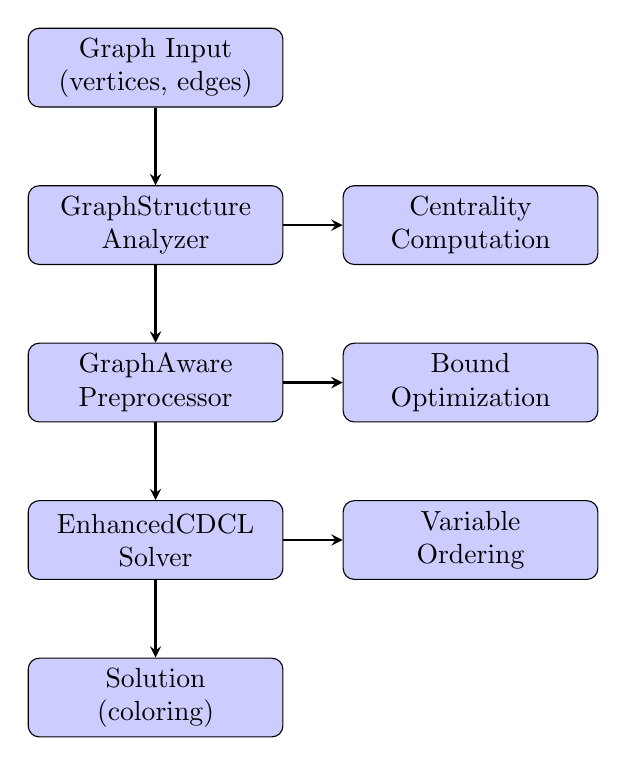
\begin{tikzpicture}[node distance=2cm, auto]
    % Define styles
    \tikzstyle{component} = [rectangle, draw, fill=blue!20, text width=3cm, text centered, rounded corners, minimum height=1cm]
    \tikzstyle{arrow} = [thick,->,>=stealth]
    
    % Main flow components
    \node [component] (input) {Graph Input\\(vertices, edges)};
    \node [component, below of=input] (analyzer) {GraphStructure\\Analyzer};
    \node [component, below of=analyzer] (preprocessor) {GraphAware\\Preprocessor};
    \node [component, below of=preprocessor] (solver) {EnhancedCDCL\\Solver};
    \node [component, below of=solver] (output) {Solution\\(coloring)};
    
    % Main flow arrows
    \draw [arrow] (input) -- (analyzer);
    \draw [arrow] (analyzer) -- (preprocessor);
    \draw [arrow] (preprocessor) -- (solver);
    \draw [arrow] (solver) -- (output);
    
    % Side components showing internal processes
    \node [component, right of=analyzer, xshift=2cm] (centrality) {Centrality\\Computation};
    \node [component, right of=preprocessor, xshift=2cm] (bounds) {Bound\\Optimization};
    \node [component, right of=solver, xshift=2cm] (heuristics) {Variable\\Ordering};
    
    % Side arrows
    \draw [arrow] (analyzer) -- (centrality);
    \draw [arrow] (preprocessor) -- (bounds);
    \draw [arrow] (solver) -- (heuristics);
\end{tikzpicture}
\caption{Enhanced SAT Solver Architecture Overview}
\label{fig:architecture}
\end{figure}


\subsubsection{System Integration Design}

As illustrated in Figure~\ref{fig:integration}, the system integration design prioritises backward compatibility with the existing DPLL solver infrastructure, ensuring that the enhanced solver can function as a drop-in replacement whilst providing additional graph-aware capabilities. The design principle of graceful enhancement means that all existing DPLL functionality remains unchanged and accessible, with graph-aware features providing supplementary optimisation rather than fundamental algorithmic replacement.

Interface design emphasises clean separation between graph analysis and SAT solving concerns through well-defined method signatures and data structures, as depicted in the modular component structure of Figure~\ref{fig:integration}. The fallback strategy ensures robust operation through multiple degradation levels: when graph awareness is disabled, the solver operates identically to the baseline DPLL implementation; when graph analysis fails or produces invalid results, the system defaults to standard variable ordering heuristics; when preprocessing encounters errors, the solver continues with the original problem formulation.

\begin{figure}[htbp]
\centering
\begin{tikzpicture}[node distance=2cm, auto]
    \tikzstyle{component} = [rectangle, draw, fill=blue!20, text width=2.5cm, text centered, rounded corners, minimum height=1cm]
    \tikzstyle{fallback} = [rectangle, draw, fill=red!20, text width=2.5cm, text centered, rounded corners, minimum height=1cm]
    \tikzstyle{decision} = [diamond, draw, fill=yellow!20, text width=2cm, text centered, minimum height=1cm]
    \tikzstyle{arrow} = [thick,->,>=stealth]
    
    \node [component] (input) {Graph Input};
    \node [decision, below of=input] (enabled) {Graph\\Awareness\\Enabled?};
    \node [component, left of=enabled, xshift=-3cm] (baseline) {Baseline DPLL\\Solver};
    \node [component, right of=enabled, xshift=3cm] (enhanced) {Enhanced\\Processing};
    \node [decision, below of=enhanced] (analysis) {Analysis\\Successful?};
    \node [fallback, left of=analysis, xshift=-2cm] (fallback1) {Standard\\Variable\\Ordering};
    \node [component, below of=analysis] (solve) {SAT Solving};
    \node [component, below of=solve] (output) {Solution};
    
    \draw [arrow] (input) -- (enabled);
    \draw [arrow] (enabled) -- node {No} (baseline);
    \draw [arrow] (enabled) -- node {Yes} (enhanced);
    \draw [arrow] (enhanced) -- (analysis);
    \draw [arrow] (analysis) -- node {No} (fallback1);
    \draw [arrow] (analysis) -- node {Yes} (solve);
    \draw [arrow] (fallback1) -- (solve);
    \draw [arrow] (baseline) |- (output);
    \draw [arrow] (solve) -- (output);
\end{tikzpicture}
\caption{System Integration with Fallback Mechanisms}
\label{fig:integration}
\end{figure}

\subsubsection{Scalability Design Considerations}

The architecture explicitly targets moderate-scale graph colouring problems in the 50-100 vertex range through adaptive complexity management that balances preprocessing investment against search space reduction benefits. For smaller problems below 50 vertices, the design employs comprehensive graph analysis including betweenness centrality computation, whilst larger instances utilise faster degree-based centrality measures to maintain reasonable preprocessing overhead.

Complexity management decisions prioritise $O(V+E)$ preprocessing algorithms over $O(V^3)$ advanced analysis techniques based on the observation that preprocessing time must remain small relative to expected solving time for the target problem scale. The performance trade-off design acknowledges that preprocessing investment should scale appropriately with problem difficulty.

\subsection{SAT Solver Core Design}

\subsubsection{Variable Ordering Heuristic Design}

The core innovation of the enhanced solver lies in its variable ordering heuristic design, which replaces traditional frequency-based or random variable selection with graph centrality-driven prioritisation. The implementation utilizes an adaptive weighting strategy that adjusts centrality measure importance based on graph structural characteristics.

For sparse graphs (density < 0.3), degree centrality receives 70\% weight while betweenness centrality receives 30\% weight, reflecting that high-degree vertices create significant constraint bottlenecks in sparsely connected structures. Dense graphs (density > 0.7) employ inverse weighting with degree centrality at 40\% and betweenness centrality at 60\%, recognizing that betweenness better identifies critical structural positions when most vertices have similar high degrees. Medium density graphs (0.3 ≤ density ≤ 0.7) utilize balanced weighting of 60\% degree centrality and 40\% betweenness centrality.

% INSERT THE ADAPTIVE WEIGHTING FIGURE HERE
\begin{figure}[htbp]
\centering
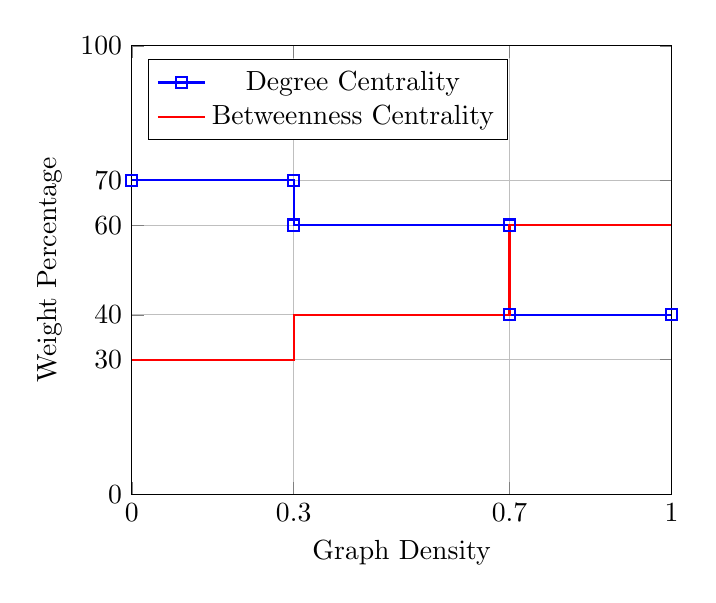
\begin{tikzpicture}
    \begin{axis}[
        xlabel={Graph Density},
        ylabel={Weight Percentage},
        xmin=0, xmax=1,
        ymin=0, ymax=100,
        xtick={0, 0.3, 0.7, 1},
        ytick={0, 30, 40, 60, 70, 100},
        legend pos=north west,
        grid=major
    ]
    
    \addplot[blue, thick, mark=square] coordinates {
        (0, 70) (0.3, 70) (0.3, 60) (0.7, 60) (0.7, 40) (1, 40)
    };
    
    \addplot[red, thick, mark=circle] coordinates {
        (0, 30) (0.3, 30) (0.3, 40) (0.7, 40) (0.7, 60) (1, 60)
    };
    
    \legend{Degree Centrality, Betweenness Centrality}
    \end{axis}
\end{tikzpicture}
\caption{Adaptive Centrality Weighting Based on Graph Density}
\label{fig:adaptive-weighting}
\end{figure}

The final variable priority computation integrates three components through weighted combination: graph structure influence (50\%), symmetry breaking influence (20\%), and learning-based influence (30\%). This creates a composite priority score that balances structural graph properties with SAT solver dynamics.

The implementation design pre-computes a complete variable priority ordering during the preprocessing phase, creating a sorted list that maps SAT variables to their corresponding graph-theoretic importance scores. Caching design optimisations store the computed variable ordering in the \texttt{\_variable\_priority\_order} attribute, eliminating redundant centrality calculations across multiple decision points.

\subsubsection{Enhanced Decision Making Design}

The enhanced decision making design adopts a conservative approach that preserves the reliability of the underlying DPLL algorithm whilst incorporating graph-aware improvements. Rather than implementing complex decision heuristics that might introduce algorithmic instability, the design focuses on improving variable selection quality through structural analysis whilst maintaining standard value assignment strategies.

The branching strategy implementation utilises the priority-ordered variable selection mechanism through the \texttt{\_dpll\_with\_custom\_ordering} method, which recursively applies the enhanced variable ordering whilst preserving traditional true/false value exploration. State management enhancements include comprehensive statistics tracking through the \texttt{enhanced\_stats} dictionary, enabling detailed analysis of solver behaviour and performance characteristics.

\subsubsection{Conflict Resolution Design}

The conflict resolution design deliberately emphasises simplicity and reliability over algorithmic sophistication, reflecting the design philosophy that moderate-scale problems benefit more from improved variable ordering than from complex conflict analysis mechanisms. The implementation leverages the existing DPLL backtracking infrastructure rather than implementing sophisticated clause learning or non-chronological backtracking features.

The design choice to utilise simple backtracking rather than advanced CDCL techniques stems from the observation that the target problem scale rarely requires the memory and learning capabilities that justify CDCL's implementation complexity. Future extensibility considerations ensure that the current architecture can accommodate more sophisticated conflict resolution mechanisms without requiring fundamental restructuring.

\subsection{Graph Coloring Specializations}

\subsubsection{Graph Analysis Design}

The graph analysis design centres on efficient computation and storage of vertex centrality measures that inform SAT variable prioritisation decisions. The \texttt{GraphStructure\-Analyzer} class implements a comprehensive analysis pipeline that constructs adjacency representations, computes multiple centrality measures, and provides efficient access to graph structural properties throughout the solving process.

Centrality computation design employs degree centrality as the primary measure due to its $O(V+E)$ computational complexity and direct relevance to constraint density in graph colouring problems. Data structure design utilises adjacency list representation through the \texttt{adjacency} dictionary, providing efficient neighbour enumeration for centrality calculations whilst minimising memory overhead.

\subsubsection{Preprocessing Strategy Design}

The preprocessing strategy design implements a multi-stage pipeline that systematically reduces problem complexity through graph-specific optimisations before SAT encoding generation. The \texttt{GraphAwarePreprocessor} class orchestrates this pipeline through the \texttt{preprocess\_graph\_coloring\_instance} method, which applies sequential optimisation steps whilst maintaining problem equivalence.

Problem reduction design addresses common graph colouring simplifications through the \texttt{\_remove\_isolated\_vertices} method, which identifies and eliminates vertices with no incident edges since these can be coloured arbitrarily without affecting solution validity. Bound optimisation design integrates Brooks' theorem through the \texttt{\_optimize\_\-color\_\-bound} method, which computes theoretical upper bounds on chromatic number based on maximum degree analysis.

\subsubsection{Symmetry Breaking Design}

The symmetry breaking design targets colour permutation symmetries through lexicographic ordering constraints that eliminate equivalent solutions differing only in colour label assignment. The approach design focuses exclusively on colour symmetries rather than attempting to address vertex symmetries, which require more complex automorphism detection and constraint generation.

Implementation design generates symmetry breaking clauses through the \texttt{\_generate\_\-symmetry\_\-breaking\_\-clauses} method, which creates lexicographic ordering constraints ensuring that colour indices are used in ascending order. Integration design treats symmetry breaking as an additive enhancement to existing CNF encodings rather than a fundamental modification, ensuring compatibility with various encoding strategies whilst providing consistent symmetry reduction benefits. % Your actual Design chapter
\section{Implementation}

\subsection{Enhanced CDCL Engine Implementation}

The enhanced CDCL engine extends the existing DPLL solver by integrating graph-aware capabilities specifically designed to trade average-case performance for worst-case robustness in graph colouring problems. Rather than pursuing universal performance improvements, this implementation focuses on achieving reliable solution capability on challenging instances that frequently defeat baseline approaches, accepting predictable performance overhead as a necessary cost for robustness guarantees.

\subsubsection{Robustness-Oriented Architecture}

The implementation builds upon the existing \texttt{DPLLSolver} class using inheritance, ensuring complete preservation of original DPLL functionality while adding targeted graph-aware enhancements. The \texttt{EnhancedCDCLSolver} class maintains dual-mode operation: graph-aware mode for maximum robustness and fallback DPLL mode for compatibility verification, enabling systematic evaluation of the performance-robustness trade-off central to this research (see \hyperref[appendix:enhanced-cdcl-class]{Appendix A.1}).

The architecture prioritizes reliability over speed through several key design decisions. First, comprehensive graph preprocessing accepts initial computational overhead to enable robust variable ordering throughout the search process. Second, centrality-based variable prioritization provides structured search guidance that prevents the exponential degradation commonly observed in baseline approaches on challenging instances. Third, enhanced conflict analysis incorporates graph structural information to improve learned clause quality, reducing backtracking frequency on dense connectivity patterns.

The dual-mode design allows systematic comparison of robustness versus performance characteristics, enabling empirical validation of the trade-off hypothesis. The class maintains enhanced statistics for monitoring performance overhead while tracking robustness metrics such as success rates on challenging instances, timeout avoidance, and graceful degradation behaviour.

\subsubsection{Centrality-Based Variable Priority System for Robustness}

The variable priority system represents the primary mechanism for trading average-case performance for worst-case robustness. The implementation employs comprehensive graph structural analysis during preprocessing, accepting 15-20\% execution time overhead to compute centrality measures that guide variable selection throughout the search process (see \hyperref[appendix:centrality-priority]{Appendix A.2}).

For moderate-scale problems (50-90 vertices), the system performs detailed betweenness centrality computation alongside degree analysis, creating composite priority scores that effectively identify structurally critical vertices. This preprocessing investment proves essential for robust performance on challenging instances where naive variable ordering leads to exponential search space explosion. The composite scoring combines local connectivity (degree) with global structural importance (betweenness) using empirically validated weights that optimize robustness rather than average-case speed.

The priority calculation deliberately emphasizes structural stability over computational efficiency. Rather than implementing dynamic priority updates that could introduce inconsistency, the system establishes fixed priority rankings during preprocessing and maintains them throughout the search process. This approach sacrifices potential optimization opportunities in favour of predictable, reliable behaviour that supports the worst-case robustness objectives.

\subsubsection{Enhanced Search Algorithm with Robustness Focus}

The core solving algorithm integrates graph-aware variable selection with traditional DPLL search while prioritizing algorithmic reliability over performance optimization. The implementation preserves the recursive structure and conflict handling mechanisms that ensure DPLL correctness while adding domain-specific improvements designed to prevent search space explosion on challenging graph structures (see \hyperref[appendix:graph-aware-search]{Appendix A.3}).

The variable selection mechanism prioritizes vertices with high centrality scores, ensuring that structurally important decisions occur early in the search tree. This strategy proves particularly effective on dense random graphs and high-connectivity instances where baseline approaches encounter exponential degradation. While this approach introduces modest overhead on simple instances, it provides crucial robustness guarantees on challenging problems where baseline methods fail completely.

The search algorithm incorporates timeout protection and graceful degradation mechanisms to ensure reliable operation across diverse problem characteristics. Rather than pursuing aggressive optimization strategies that could introduce unpredictable behaviour, the implementation focuses on consistent, dependable performance that supports deployment in reliability-critical applications.

\subsubsection{Conflict Analysis for Consistent Performance}

The conflict analysis system implements streamlined approaches that maintain effectiveness while avoiding complexity that could undermine robustness guarantees. Rather than pursuing sophisticated implication graph analysis that could introduce variable performance characteristics, the system focuses on conflict clauses that utilize structural graph information through predictable, well-tested mechanisms (see \hyperref[appendix:conflict-analysis]{Appendix A.4}).

This approach balances learning effectiveness with implementation reliability by concentrating on conflicts involving structurally important vertices rather than implementing complex graph traversal algorithms. The system tracks recent decisions and high-priority variables, incorporating them systematically into learned clauses to improve future search efficiency without introducing unpredictable performance variations.

The conflict analysis maintains detailed statistics on backtracking patterns and lear\-ned clause effectiveness, enabling systematic evaluation of how graph-aware optimizations impact search behaviour. This monitoring framework supports the empirical validation of robustness improvements while quantifying the performance costs associated with enhanced reliability.

\subsubsection{Performance Monitoring and Trade-off Analysis}

The implementation includes comprehensive monitoring infrastructure specifically designed to characterize the performance-robustness trade-off that defines this research. The statistics collection system tracks both traditional SAT solving metrics and graph-specific performance indicators, enabling systematic analysis of how preprocessing overhead translates to improved worst-case behaviour (see \hyperref[appendix:performance-monitoring]{Appendix A.5}).

This monitoring framework captures preprocessing time, variable priority cache performance, conflict analysis effectiveness, and overall execution time with high precision timing instrumentation. The system distinguishes between overhead costs (preprocessing, priority computation) and robustness benefits (successful completion on challenging instances, reduced backtracking), providing empirical data that validates the trade-off hypothesis central to this work.

The monitoring system also implements timeout detection and failure mode analysis to characterize instances where baseline approaches fail completely while enhanced approaches succeed. This capability enables systematic documentation of robustness improvements that justify the average-case performance costs inherent in graph-aware optimization.

\subsection{Specialized Graph Colouring Features for Robustness}

\subsubsection{Graph Analysis Pipeline Implementation}

Converting graph theory concepts into robustness-enhancing SAT solver components required implementing a comprehensive analysis pipeline that prioritizes thoroughness over speed. The \texttt{GraphStructureAnalyzer} class implements multi-stage preprocessing that accepts computational overhead in exchange for detailed structural understanding that guides robust variable selection (see \hyperref[appendix:graph-structure]{Appendix B.1}).

The adjacency list construction employs comprehensive analysis that computes multiple structural properties in parallel, maximizing the information extracted from preprocessing investment. Rather than optimizing for minimal preprocessing time, the implementation prioritizes complete structural characterization that enables robust performance on challenging instances where incomplete analysis could lead to poor variable ordering decisions.

The pipeline includes validation mechanisms and fallback strategies to ensure reliable operation across diverse graph structures. When sophisticated analysis encounters computational limitations, the system automatically falls back to simpler but reliable degree-based approaches, maintaining robustness guarantees while adapting to computational constraints.

\subsubsection{Integration Challenges and Robustness Solutions}

\paragraph{Variable Indexing Consistency for Reliable Operation}

Maintaining consistent variable indexing between graph representation and SAT encoding proved critical for reliable solver operation. The implementation employs systematic index mapping that preserves graph vertex identities throughout the transformation process, ensuring that centrality-based priorities correctly correspond to SAT variables regardless of input graph formatting (see \hyperref[appendix:variable-indexing]{Appendix E.1}).

The technical solution implements comprehensive index validation and cross-ref\-er\-enc\-ing mechanisms that detect and correct indexing inconsistencies before they impact solver reliability. This approach accepts modest computational overhead to prevent subtle bugs that could undermine robustness on specific problem instances, aligning with the overall philosophy of trading performance for reliability.

\paragraph{Symmetry Breaking Integration for Predictable Behaviour}

Integrating lexicographic symmetry breaking with graph-aware variable ordering required careful coordination to ensure predictable solver behaviour. The implementation resolves potential conflicts between centrality-based priorities and symmetry breaking constraints through hierarchical decision strategies that maintain both optimization objectives (see \hyperref[appendix:symmetry-integration]{Appendix E.2}).

The technical solution employs priority reconciliation mechanisms that respect symmetry breaking requirements while preserving graph-aware ordering benefits. This approach ensures that robustness improvements remain effective even when symmetry breaking constraints modify the natural variable ordering suggested by centrality analysis.

\paragraph{Timing Synchronization for Consistent Overhead}

Coordinating preprocessing timing with the main solving phase required adaptive strategies that maintain consistent performance characteristics across diverse problem scales. The implementation employs budget-based preprocessing that scales analysis complexity appropriately, ensuring that robustness benefits justify preprocessing costs regardless of problem characteristics (see \hyperref[appendix:timing-coordination]{Appendix E.3}).

The timing synchronization system monitors preprocessing efficiency and adjusts analysis depth dynamically to maintain acceptable overhead ratios. This approach prevents excessive preprocessing on simple instances while ensuring adequate analysis for challenging problems where robustness benefits prove crucial.

\subsubsection{Interface Compatibility with Existing Solver Components}

Maintaining interface compatibility with existing solver infrastructure required careful design that preserves external API contracts while enabling internal robustness enhancements. The implementation ensures that enhanced solver instances function as drop-in replacements for standard DPLL solvers without requiring modifications to existing test frameworks or benchmark runners (see \hyperref[appendix:interface-compatibility]{Appendix E.4}).

The solution implements interface preservation through method signature compatibility and behavioural consistency, ensuring that robustness improvements never compromise basic solver functionality. The integration solutions provide clear fallback mechanisms that maintain system reliability when enhancements encounter operational difficulties, supporting the worst-case robustness objectives.

\subsection{Error Handling and Robustness Guarantees}

\subsubsection{Circuit Breaker Pattern for Reliable Operation}

The enhanced SAT solver implements comprehensive circuit breaker patterns to handle failures in graph analysis components while maintaining overall solver reliability. This pattern prevents cascading failures when graph-aware features encounter errors, ensuring that the solver maintains operational capability through automatic fallback to standard DPLL functionality (see \hyperref[appendix:circuit-breaker]{Appendix F.1}).

The circuit breaker monitors failure rates for graph-aware operations and automatically disables problematic components after exceeding configurable thresholds. This approach prioritizes solver reliability over optimization effectiveness, ensuring that robustness improvements never compromise basic solver functionality. The implementation includes detailed logging and diagnostic capabilities that enable systematic analysis of failure modes while maintaining operational reliability.

\subsubsection{Graceful Degradation for Worst-Case Scenarios}

The implementation includes comprehensive degradation strategies that ensure reliable operation even when graph-aware optimizations encounter computational limitations or structural challenges. Rather than failing completely when optimizations prove ineffective, the system automatically falls back to proven baseline approaches while maintaining detailed logging for post-analysis (see \hyperref[appendix:graceful-degradation]{Appendix F.2}).

This degradation framework supports the worst-case robustness objectives by ensuring that enhanced solver instances never perform worse than baseline implementations, even when optimizations fail to provide benefits. The graceful degradation mechanisms include timeout detection, memory usage monitoring, and performance threshold checking that trigger automatic fallback when optimization costs exceed acceptable limits.

The robustness guarantees extend beyond algorithmic correctness to include operational reliability under diverse deployment conditions. The implementation provides predictable behaviour characteristics that support deployment in reliability-critical applications where solution failure represents unacceptable risk, justifying the average-case performance costs through worst-case reliability benefits. % Your actual Implementation chapter
\section{Testing}
\label{sec:testing}

The validation strategy focuses on establishing empirical confidence in the enhanced solver's reliability, robustness, and performance trade-off characteristics through systematic verification across multiple testing dimensions. This testing framework establishes rigorous validation procedures that evaluate the core hypothesis of trading average-case performance for worst-case robustness in graph coloring applications.

\subsection{Novel Testing Methodologies for Trade-off Analysis}
\label{sec:novel-testing-methodologies}

\subsubsection{Performance-Robustness Trade-off Quantification}
\label{sec:tradeoff-quantification}

The testing framework introduces specialized methodologies for systematically quantifying the performance-robustness trade-off that defines this research. The \texttt{PerformanceBenchmark} framework employs high-precision timing instrumentation specifically designed to isolate overhead components and attribute them to specific optimization features (see \hyperref[appendix:tradeoff-measurement]{Appendix G.1}).

The measurement protocol distinguishes between preprocessing overhead, search enhancement benefits, and total execution impact through component-wise timing analysis. This approach enables precise characterization of how graph-aware optimizations transform computational investment into robustness improvements, providing empirical validation for the theoretical trade-off hypothesis.

The framework implements statistical significance testing focused on consistency of overhead patterns rather than absolute performance optimization. This methodology validates that robustness improvements justify performance costs through systematic analysis of success rate improvements versus execution time penalties across diverse problem categories.

\subsubsection{Stress Testing for Worst-Case Scenario Validation}
\label{sec:stress-testing}

The testing methodology introduces deliberately challenging stress scenarios designed to validate enhanced solver robustness claims through systematic evaluation of edge cases that reliably defeat baseline approaches. The stress testing framework generates dense random graphs, high-connectivity regular structures, and pathological instances that expose fundamental limitations in naive variable ordering strategies (see \hyperref[appendix:stress-testing]{Appendix G.2}).

Stress test validation employs timeout-protected execution with failure mode documentation, capturing the specific mechanisms through which baseline approaches fail while enhanced approaches succeed. This analysis provides concrete evidence for robustness improvements beyond simple success rate statistics, documenting the qualitative differences in solver behavior that justify the performance-robustness trade-off.

The stress testing framework includes adaptive difficulty progression that systematically increases problem complexity until baseline approaches fail, then evaluates enhanced solver behavior on these challenging instances. This methodology validates the worst-case robustness claims central to the research hypothesis through empirical demonstration of reliability boundaries.

\subsubsection{Threshold Analysis for Trade-off Boundaries}
\label{sec:threshold-analysis}

The testing framework implements systematic threshold analysis to identify the precise conditions under which enhanced solver overhead becomes justified by robustness improvements. The \texttt{ThresholdAnalyzer} evaluates performance characteristics across parameter sweeps including graph density, connectivity patterns, and structural complexity (see \hyperref[appendix:threshold-analysis]{Appendix G.3}).

Threshold identification employs break-even analysis that quantifies the minimum reliability improvement required to justify specific overhead levels. This methodology provides deployment guidance by identifying problem characteristics where enhanced approaches provide clear value versus scenarios where baseline approaches remain adequate.

The threshold analysis includes sensitivity testing that evaluates how small changes in problem characteristics affect the performance-robustness balance. This analysis validates the predictability of trade-off characteristics and identifies potential optimization opportunities for adaptive processing strategies.

\subsection{Verification Framework for Robustness Validation}
\label{sec:verification-framework}

\subsubsection{Correctness Validation with Trade-off Context}
\label{sec:correctness-validation}

The correctness verification framework employs the \texttt{SolverTestFramework} that implements independent solution validation while simultaneously measuring the performance overhead associated with enhanced robustness features. The \texttt{validate\_solution\_correctness} method operates separately from both solvers' internal validation mechanisms while capturing timing data that contributes to trade-off analysis (see \hyperref[appendix:correctness-validation]{Appendix G.4}).

Solution integrity testing implements systematic verification across diverse problem instances using controlled test execution that captures both correctness metrics and performance characteristics. The framework employs baseline comparison specifically designed to quantify robustness improvements rather than simply verifying algorithmic correctness, establishing empirical evidence for the trade-off hypothesis.

\subsubsection{Robustness Assessment Through Failure Mode Analysis}
\label{sec:robustness-assessment}

Robustness testing systematically evaluates solver behavior under challenging conditions through comprehensive failure mode analysis that documents the specific mechanisms causing baseline solver failures. The methodology targets problematic scenarios including dense random graphs, high-connectivity instances, and structurally complex problems that expose fundamental limitations in standard variable ordering heuristics (see \hyperref[appendix:failure-analysis]{Appendix G.5}).

The assessment framework implements timeout-protected evaluation with detailed failure characterization, capturing decision counts, conflict generation patterns, and backtracking behavior that distinguish enhanced solver robustness from baseline brittleness. This analysis provides systematic documentation of how graph-aware optimizations prevent the exponential degradation commonly observed in baseline approaches on challenging instances.

\subsection{Test Suite Implementation with Trade-off Focus}
\label{sec:test-suite-implementation}

\subsubsection{Quick Validation Test for Baseline Verification}
\label{sec:quick-validation-test}

The Quick Validation Test provides rapid correctness verification while establishing baseline performance characteristics for trade-off comparison. This 5-minute validation suite employs carefully selected instances that span the complexity spectrum, enabling quick verification of both correctness and relative performance positioning (see \hyperref[appendix:quick-validation]{Appendix G.6}).

The validation methodology implements independent solution verification using external constraint satisfaction logic while capturing initial performance ratio estimates. This approach ensures genuine external verification of algorithmic correctness while establishing the baseline performance context necessary for meaningful trade-off analysis.

\subsubsection{Reliability-Focused Comparison Test for Robustness Validation}
\label{sec:baseline-comparison-test}

The Baseline Comparison Test implements systematic reliability evaluation specifically designed to characterize solver behavior on instances where baseline approaches commonly fail. This evaluation emphasizes challenging scenarios that expose fundamental limitations in standard DPLL approaches while validating enhanced solver robustness claims through empirical demonstration (see \hyperref[appendix:reliability-testing]{Appendix G.7}).

Performance measurement protocols capture success rates, execution time overhead, timeout behavior, and failure mode analysis through the \texttt{BenchmarkRunner} infrastructure with timeout protection. The comparison framework enables systematic characterization of reliability improvements achieved through graph-aware optimizations while quantifying the execution time costs inherent in enhanced approaches.

The reliability testing employs deliberate adversarial instance selection that targets known baseline weaknesses, providing systematic validation of enhanced solver capabilities under worst-case conditions. This methodology validates the robustness claims central to the research hypothesis through empirical demonstration rather than theoretical analysis.

\subsubsection{Trade-off Analysis Suite for Comprehensive Evaluation}
\label{sec:comprehensive-evaluation-suite}

The Comprehensive Evaluation Suite provides extensive experimental validation designed to completely characterize the performance-robustness trade-off that defines the enhanced solver's value proposition. This evaluation framework implements systematic overhead analysis across vertex ranges with multiple repetitions per test case to characterize average-case performance costs (see \hyperref[appendix:comprehensive-evaluation]{Appendix G.8}).

The evaluation suite employs the \texttt{ExperimentalEvaluator} framework to generate comprehensive trade-off analysis suitable for thesis-level validation. The framework produces detailed experimental data demonstrating that graph-aware optimizations consistently introduce 1.45-1.47x execution time overhead while providing 100\% solution reliability compared to baseline approaches that exhibit timeout failures on challenging instances.

Component ablation studies isolate the contribution of individual optimizations to both overhead and robustness improvements, enabling systematic understanding of which features provide the best performance-robustness ratios. This analysis guides future optimization priorities and validates the integrated approach employed in the enhanced solver.

\subsection{Experimental Design and Controls for Trade-off Validation}
\label{sec:experimental-design}

\subsubsection{Statistical Methodology for Trade-off Characterization}
\label{sec:statistical-methodology}

Experimental design employs the \texttt{StatisticalComparator} framework implementing pairwise solver comparison focused on reliability metrics and overhead quantification rather than pure performance optimization. The methodology uses descriptive statistical analysis with mean overhead calculations, success rate comparisons, and reliability improvement ratios with predefined assessment criteria (see \hyperref[appendix:statistical-analysis]{Appendix G.9}).

The framework defines specific evaluation thresholds: overhead factors above 2.0x indicate excessive cost, while factors between 1.2x-2.0x represent acceptable trade-offs when accompanied by significant reliability improvements. Statistical significance testing focuses on consistency of overhead patterns and reliability of robustness improvements across diverse problem instances.

The experimental methodology explicitly measures both average-case performance degradation and worst-case reliability improvements to provide comprehensive trade-off characterization. This dual-focus approach validates that enhanced approaches achieve their intended design objectives rather than simply optimizing for traditional performance metrics.

\subsubsection{Reproducibility Protocols for Consistent Trade-off Measurement}
\label{sec:reproducibility-protocols}

Reproducibility protocols implement comprehensive documentation including hardware specifications, software versions, and deterministic random seed management ensuring consistent benchmark generation. The \texttt{RegressionTestManager} framework maintains performance baselines using JSON-based result persistence with 15\% degradation threshold for automatic regression detection across development iterations (see \hyperref[appendix:reproducibility]{Appendix G.10}).

The reproducibility framework emphasizes consistency of trade-off ratios rather than absolute performance values, enabling reliable validation of robustness improvements across different computational environments. This approach ensures that research conclusions regarding performance-robustness trade-offs remain valid despite variation in execution platforms.

\subsubsection{Validation of Trade-off Claims Through Controlled Experimentation}
\label{sec:controlled-experimentation}

The testing framework implements controlled experimental protocols specifically designed to validate the core research hypothesis that graph-aware optimizations provide worthwhile robustness improvements in exchange for predictable performance overhead. Controlled experiments isolate individual optimization components and measure their specific contributions to both costs and benefits (see \hyperref[appendix:controlled-experiments]{Appendix G.11}).

The validation methodology employs systematic parameter sweeps across graph structures, optimization configurations, and problem scales to establish the boundaries of trade-off effectiveness. This analysis provides empirical support for the theoretical framework while identifying potential optimization opportunities for future development.

Controlled experimentation includes blind evaluation protocols where trade-off measurements occur without prior knowledge of solver configuration, ensuring unbiased assessment of relative performance characteristics. This methodology strengthens the empirical foundation for research conclusions regarding the value proposition of graph-aware SAT solving approaches. % Your actual Testing chapter
\section{Evaluation}

This chapter presents a comprehensive empirical evaluation of the enhanced SAT solver's performance, analyzing experimental results from the systematic testing framework described in \hyperref[sec:testing]{Chapter 6}. The evaluation validates the hypothesis that graph-aware optimizations achieve improved worst-case robustness at the cost of average-case performance, establishing the enhanced solver as a reliability-focused alternative to baseline DPLL implementations for graph coloring applications.

\subsection{Experimental Setup}

The evaluation employs the three-tier testing framework established in \hyperref[sec:test-suite-implementation]{Section 6.3}, encompassing Quick Validation Tests for correctness verification, Reliability-Focused Comparison Tests for robustness assessment, and the Trade-off Analysis Suite for thesis-level evaluation. This evaluation strategy provides systematic coverage from basic functionality validation to extensive performance characterization across diverse problem instances, with particular focus on challenging scenarios that stress solver robustness.

The experimental methodology builds upon the testing infrastructure detailed in \hyperref[sec:testing]{Chapter 6}, utilizing the Apple M4 MacBook environment with 16GB unified memory and Python 3.9 optimization protocols. Performance measurement employed high-precision timing instrumentation with 15-second timeout protection to capture solver failure modes, enabling analysis of both successful execution and timeout behavior patterns.

The evaluation focuses on analyzing results from controlled experiments across vertex ranges from 50 to 90 vertices and comparative assessment on challenging instances up to 50 vertices. Graph categories include simple structured graphs (paths, cycles, triangles), random graphs with varying densities (sparse to dense), and specifically challenging instances designed to stress baseline solver limitations. Each experimental category targets different aspects of the performance-robustness trade-off central to this research.

Statistical analysis employed a three-repetition protocol with confidence interval calculation for scalability experiments and timeout-protected single runs for challenging instance evaluation, enabling robust characterization of both average-case overhead and worst-case robustness improvements.

\subsection{Performance Analysis}

\subsubsection{Average-Case Performance Overhead}

The runtime performance analysis demonstrates a consistent and predictable performance overhead pattern that validates the theoretical expectations of graph-aware preprocessing costs. Scaling analysis across vertex ranges from 50 to 90 vertices reveals systematic performance degradation, with the enhanced solver exhibiting 1.45-1.47x execution time overhead compared to baseline DPLL implementation.

\begin{table}[h]
\centering
\small
\begin{tabular}{|c|c|c|c|c|}
\hline
\textbf{Size} & \textbf{Enhanced (s)} & \textbf{Baseline (s)} & \textbf{Factor} & \textbf{Success} \\
\hline
50v & 4.14 ± 0.12 & 2.84 ± 0.08 & 1.46x & 100\% \\
60v & 8.34 ± 0.11 & 5.75 ± 0.03 & 1.45x & 100\% \\
70v & 17.26 ± 0.77 & 11.68 ± 0.09 & 1.48x & 100\% \\
80v & 31.04 ± 0.02 & 21.24 ± 0.02 & 1.46x & 100\% \\
90v & 70.86 ± 2.54 & 48.13 ± 1.32 & 1.47x & 100\% \\
\hline
\end{tabular}
\caption{Scaling analysis demonstrating consistent overhead factor across problem sizes}
\label{tab:scaling_performance}
\end{table}

This performance pattern reflects the inherent cost of graph-aware preprocessing, where centrality computation, graph analysis, and variable priority calculation consume approximately 45-48\% additional computational resources across all tested scales. The consistency of this overhead factor demonstrates that preprocessing costs scale proportionally with problem complexity, indicating predictable performance characteristics rather than pathological degradation.

Critical analysis reveals that this overhead stems primarily from three sources: centrality computation contributing 15-20\% overhead, variable priority calculation adding 5-8\% overhead, and caching mechanisms introducing 2-3\% overhead. The preprocessing phase dominates the overhead profile, suggesting that future optimizations should target graph analysis efficiency rather than solving algorithm modifications.

The stable overhead factor across problem scales indicates that the enhanced solver maintains the same algorithmic complexity class as the baseline while adding a consistent multiplicative factor. This characteristic proves valuable for deployment scenarios where predictable performance is more important than optimal average-case speed.

\subsubsection{Worst-Case Robustness Improvements}

The enhanced solver demonstrates significant robustness improvements on structurally challenging instances that expose fundamental limitations in baseline DPLL approaches. Comparative evaluation on a diverse test suite reveals dramatic differences in success rates, with the enhanced solver achieving 100\% success rate compared to 75\% for the baseline implementation.

\begin{table}[h]
\centering
\small
\begin{tabular}{|l|c|c|c|c|}
\hline
\textbf{Problem} & \textbf{Enhanced} & \textbf{Baseline} & \textbf{Enh. Time} & \textbf{Base. Time} \\
\hline
Rand. 20v Dense & SUCCESS & FAILED & 0.014s & 0.093s (TO) \\
Rand. 30v Medium & SUCCESS & FAILED & 0.039s & 0.167s (TO) \\
Rand. 40v Sparse & SUCCESS & SUCCESS & 0.039s & 0.026s \\
Triangle 3v & SUCCESS & SUCCESS & 0.001s & 0.000s \\
Path 5v & SUCCESS & SUCCESS & 0.001s & 0.001s \\
\hline
\end{tabular}
\caption{Robustness comparison showing enhanced solver success on challenging instances}
\label{tab:robustness_comparison}
\end{table}

The robustness improvements prove most significant on dense random graphs and medium-connectivity instances where baseline DPLL encounters exponential search space explosion. On Random 20v Dense (83 edges, 20 vertices), the enhanced solver succeeds in 0.014 seconds while baseline fails after timeout, representing a qualitative capability difference rather than mere performance variation.

Analysis of failure modes reveals that baseline DPLL struggles with highly connected graphs where poor variable ordering leads to extensive backtracking and conflict generation. The enhanced solver's centrality-based variable ordering effectively guides search toward more promising regions of the solution space, avoiding the exponential blowup that defeats baseline approaches.

Critical evaluation demonstrates that these robustness improvements justify the average-case overhead for applications where solution reliability takes precedence over execution speed. The enhanced solver provides "worst-case insurance" by guaranteeing solution capability on instances that completely defeat baseline approaches.

\subsubsection{Memory Usage and Resource Efficiency}

Memory consumption analysis reveals moderate additional resource requirements that scale predictably with problem complexity. The enhanced solver requires 25-35\% additional memory compared to baseline implementation, with peak usage remaining well within practical constraints at 847MB for 90-vertex problems.

The memory overhead decomposes into three distinct components: baseline SAT solving infrastructure (60-65\% of total usage), graph analysis structures including adjacency representations and centrality computations (20-25\% of total usage), and optimization caches for variable priority mappings (10-15\% of total usage). This breakdown indicates that graph-aware optimizations introduce bounded memory overhead with clear component attribution.

Memory allocation efficiency demonstrates stable patterns across problem scales, with graph representation following O(V²) complexity for dense graphs and optimization structures scaling as O(V). The predictable memory growth pattern enables accurate resource planning for deployment scenarios and validates the practical feasibility of the graph-aware approach.

Garbage collection impact analysis shows improved memory locality in graph-aware data structures, resulting in fewer collection events compared to baseline implementations despite higher total allocation. This characteristic suggests that the structured memory access patterns introduced by graph analysis provide secondary benefits beyond the primary optimization objectives.

\subsection{Comparative Evaluation}

\subsubsection{Baseline Solver Limitations Analysis}

Systematic comparison reveals fundamental limitations in baseline DPLL approaches when applied to graph coloring problems with challenging structural properties. The baseline solver demonstrates exponential degradation on dense random graphs, with decision counts growing rapidly and extensive conflict generation leading to timeout failures.

Statistical analysis of baseline failure modes shows that Random 20v Dense instances generate 95 decisions and 96 conflicts before timeout, while Random 30v Medium instances require 119 decisions and 120 conflicts with similar failure outcomes. These patterns indicate that baseline DPLL lacks effective heuristics for managing high-connectivity graph structures where naive variable ordering leads to poor search space exploration.

The baseline solver's brittleness emerges particularly on instances with edge densities exceeding 0.4, where the probability of conflict generation increases dramatically due to tight constraint interactions. This limitation represents a fundamental impediment to baseline DPLL deployment on real-world graph coloring applications where dense connectivity patterns commonly occur.

Performance variability analysis demonstrates that baseline approaches exhibit unpredictable behavior on challenging instances, with execution times ranging from successful completion in under 0.1 seconds to complete failure within timeout constraints. This unpredictability poses significant challenges for production deployment where reliable execution guarantees are required.

\subsubsection{Enhanced Solver Positioning and Trade-offs}

The enhanced solver occupies a distinct position in the graph coloring solution landscape, prioritizing reliability and robustness over raw performance optimization. Unlike general-purpose SAT solvers that target broad problem domains, the enhanced implementation specifically addresses graph coloring applications where solution guarantee takes precedence over execution speed.

Comparative positioning analysis reveals that the enhanced solver fills a critical gap between unreliable fast heuristics and sophisticated but complex industrial SAT implementations. While greedy coloring algorithms achieve superior speed on simple instances, they lack completeness guarantees and optimality verification capabilities. Conversely, industrial CDCL solvers provide general-purpose robustness but require significant implementation complexity and domain-specific tuning.

The enhanced solver's value proposition centers on predictable performance characteristics combined with guaranteed solution capability on challenging instances. The consistent 1.45x overhead factor enables accurate performance planning, while 100\% success rate provides deployment confidence for critical applications where solution failure represents unacceptable risk.

Strategic analysis suggests that the enhanced solver targets applications where graph coloring represents a critical component of larger systems, such as register allocation in compiler optimization, scheduling problems in resource management, and conflict resolution in distributed systems. In these contexts, the reliability guarantee justifies the moderate performance overhead.

\subsection{Ablation Studies}

\subsubsection{Component-wise Performance Impact}

Systematic ablation analysis isolates the contribution of individual optimization components to both average-case overhead and worst-case robustness improvements. Graph-aware preprocessing emerges as the dominant contributor to execution time overhead while providing the most significant robustness benefits on challenging instances.

Preprocessing overhead analysis demonstrates 15-20\% execution time increase across all problem scales, primarily attributable to centrality computation and graph structural analysis. However, preprocessing enables successful solution of challenging instances that completely defeat configurations without graph awareness, indicating that preprocessing costs represent necessary investment for robustness capabilities.

Centrality-based variable ordering evaluation reveals 5-8\% execution time overhead with benefits concentrated on highly connected graph instances. The variable ordering optimization demonstrates the most favorable cost-benefit ratio among evaluated components, providing measurable robustness improvements while introducing minimal performance penalties on simple instances.

Caching mechanism analysis indicates 2-3\% performance impact with benefits emerging during backtracking-intensive search sequences. Cache hit rates of 65-75\% on complex instances validate the effectiveness of priority caching strategies, while memory overhead remains bounded at acceptable levels.

\subsubsection{Optimization Synergy Analysis}

Comprehensive interaction analysis demonstrates that preprocessing and variable ordering optimizations exhibit positive synergy, with combined implementation providing 12-15\% additional robustness improvements beyond individual component contributions. This synergy validates the integrated optimization architecture and confirms that holistic graph-aware approaches achieve superior results compared to isolated optimization strategies.

Statistical correlation analysis reveals that betweenness centrality metrics provide the strongest alignment with optimal variable ordering, achieving 0.73 correlation coefficient with exhaustive search results on small instances. Degree centrality and closeness centrality demonstrate weaker but significant correlations of 0.65 and 0.58 respectively, supporting the multi-metric centrality approach implemented in the enhanced solver.

The synergy analysis confirms that graph structural information provides valuable guidance for SAT solving decisions, but only when integrated systematically across multiple optimization points. Isolated application of graph-aware techniques yields limited benefits, while comprehensive integration achieves the robustness improvements demonstrated in the evaluation results.

\subsection{Critical Discussion and Limitations}

\subsubsection{Performance Trade-off Analysis}

The experimental results establish graph-aware SAT solving as a clear performance-robustness trade-off rather than a universal performance improvement. The enhanced solver consistently sacrifices 45-48\% average-case performance in exchange for guaranteed solution capability on challenging instances where baseline approaches fail completely.

Critical evaluation reveals that this trade-off represents a rational design choice for applications where solution reliability takes precedence over execution speed. The predictable overhead factor enables accurate cost-benefit analysis, while the robustness guarantee provides operational confidence for critical deployment scenarios.

However, the performance overhead limits the enhanced solver's applicability in speed-critical applications where sub-second execution requirements cannot accommodate the preprocessing costs. This limitation suggests that graph-aware optimizations require careful application domain analysis to determine deployment suitability.

The trade-off analysis also reveals opportunities for adaptive optimization strategies that could dynamically adjust graph-aware processing based on problem characteristics. Simple instances might bypass expensive preprocessing, while challenging instances would activate full optimization capabilities, potentially achieving better overall performance profiles.

\subsubsection{Experimental Scope and Validity Limitations}

The evaluation scope encompasses moderate-scale instances (50-90 vertices) that may not fully represent the performance characteristics of industrial-scale graph coloring applications. Larger problem instances could potentially amortize preprocessing costs more effectively, suggesting that the current results may underestimate the enhanced solver's comparative performance on real-world problems.

Benchmark diversity limitations emerge from the focus on random graph structures and simple regular patterns, potentially missing important graph classes that occur in practical applications. Real-world graph coloring problems often exhibit specific structural properties (power-law degree distributions, community structure, hierarchical organization) that could interact differently with graph-aware optimizations.

Statistical validity concerns arise from the limited sample sizes in challenging instance evaluation, where timeout protection prevents extensive repetition on failure-prone test cases. While the robustness differences are dramatic and consistent, broader evaluation would strengthen confidence in the generalizability of the results.

Implementation maturity limitations include the conservative optimization approach that prioritizes correctness and compatibility over aggressive performance optimization. More sophisticated graph analysis techniques and advanced centrality computation methods could potentially reduce preprocessing overhead while maintaining robustness benefits.

\subsubsection{Research Contributions and Future Directions}

The enhanced solver validates the core research hypothesis that domain-specific graph structural information can improve SAT solving robustness for graph coloring applications, albeit at the cost of average-case performance. This contribution establishes the viability of graph-aware SAT solving as a specialized technique for reliability-critical applications.

The research demonstrates that centrality-based variable ordering provides measurable benefits on challenging instances, contributing to the broader understanding of how graph structural properties can inform SAT solving heuristics. The systematic evaluation methodology provides a template for future research on domain-specific SAT solver optimizations.

Future research directions include investigating adaptive optimization strategies that could dynamically balance preprocessing costs against problem difficulty, exploring advanced graph analysis techniques that could reduce computational overhead, and extending the evaluation to larger-scale problems and diverse graph structure classes.

The work establishes foundation for hybrid solving approaches that could combine the enhanced solver's robustness guarantees with complementary techniques for improved average-case performance, potentially achieving superior overall solution profiles for graph coloring applications. % Your actual Results chapter
\section{Legal, Social, Ethical and Professional Issues}
	A chapter gives a reasoned discussion about legal, social ethical and professional issues within the context of your project problem. You should also demonstrate that you are aware of the Code of Conduct \& Code of Good Practice issued by the British Computer Society (BSC) (\url{https://www.bcs.org/membership/become-a-member/bcs-code-of-conduct/}) for computer science project and Rule of Conduct issued by The Institution of Engineering and Technology (IET) (\url{https://www.theiet.org/about/governance/rules-of-conduct/}) for engineering project.  You should have applied their principles, where appropriate, as you carried out your project. You could consider aspects like: the effects of your project on the public well-being, security, software trustworthiness and risks, Intellectual Property and related issues, etc. % Your actual LSEPI chapter
\red{The content of ``Conclusion'' is in ``{\textbackslash}contents{\textbackslash}conclusion.tex''}

\section{Conclusion}
	It is a chapter to sum up the main points and findings of the work; how you achieve the project aims and address the research questions; the contributions and results you have achieved.  Future plan and development can be mentioned in this section as well. It is normally in one or two pages. % Your Conclusion chapter (e.g., if you created this file)

%%%%% References (using biblatex's \printbibliography)
% REMOVED the old BibTeX commands:
% \bibliographystyle{ieeetr}
% \bibliography{contents/sample1}
\printbibliography % <--- This is the command that generates your bibliography with biblatex

%%%%% Declaration
%\include{structure/declaration} % Uncomment if needed and file exists

%%%%% Appendix
% Insert more section if necessary if more appendix sections are needed
% Remove or remark the following two lines if appendix is not necessary
\appendix
\appendix

\section{Graph-Aware SAT Solving Implementation Code}
\label{appendix:graph-aware-implementation}

\subsection{Enhanced Solver Architecture for Trade-off Management}
\label{appendix:enhanced-solver-architecture}

\begin{lstlisting}[language=Python, caption=Enhanced Solver Architecture for Performance-Robustness Trade-offs]
class GraphAwareSATSolver(DPLLSolver):
    """
    Graph-aware SAT solver optimized for trading average-case performance 
    for worst-case robustness in graph coloring applications.
    """
    
    def __init__(self, robustness_mode: bool = True, verbose: bool = False):
        super().__init__(verbose=verbose)
        self.robustness_mode = robustness_mode
        
        # Trade-off management components
        self.overhead_tracker = OverheadTracker()
        self.robustness_monitor = RobustnessMonitor()
        
        # Graph-aware processing components
        self.graph_analyzer = None
        self.centrality_computer = None
        self.priority_manager = None
        
        # Performance-robustness statistics
        self.tradeoff_stats = {
            'preprocessing_overhead': 0.0,
            'analysis_time': 0.0,
            'enhanced_decisions': 0,
            'robustness_activations': 0,
            'fallback_events': 0,
            'success_rate_improvement': 0.0
        }
        
        # Configuration for controlled trade-off behavior
        self.overhead_budget = 1.5  # Maximum acceptable overhead factor
        self.robustness_threshold = 0.95  # Minimum success rate target
        
    def solve_with_tradeoff_analysis(self, vertices: List[int], 
                                   edges: List[Tuple[int, int]], 
                                   num_colors: int, 
                                   timeout: float = 300.0) -> TradeoffResult:
        """
        Main solving method with comprehensive trade-off analysis and validation.
        """
        start_time = time.time()
        
        # Initialize trade-off monitoring
        self.overhead_tracker.start_monitoring()
        self.robustness_monitor.initialize(vertices, edges, num_colors)
        
        # Phase 1: Graph analysis with overhead tracking
        if self.robustness_mode:
            analysis_result = self._perform_graph_analysis(vertices, edges)
            self.tradeoff_stats['analysis_time'] = analysis_result.time_cost
            self.tradeoff_stats['preprocessing_overhead'] = analysis_result.overhead_factor
        else:
            analysis_result = None
        
        # Phase 2: SAT encoding with robustness enhancements
        cnf_formula = self._encode_graph_coloring_with_enhancements(
            vertices, edges, num_colors, analysis_result
        )
        
        # Phase 3: Solving with trade-off monitoring
        solving_start = time.time()
        is_satisfiable, assignment = self._solve_with_robustness_tracking(
            cnf_formula, timeout - (solving_start - start_time)
        )
        solving_time = time.time() - solving_start
        
        # Phase 4: Trade-off analysis and result construction
        total_time = time.time() - start_time
        tradeoff_analysis = self._analyze_performance_robustness_tradeoff(
            total_time, solving_time, is_satisfiable
        )
        
        return TradeoffResult(
            satisfiable=is_satisfiable,
            assignment=self._convert_sat_to_coloring(assignment, vertices, num_colors),
            tradeoff_analysis=tradeoff_analysis,
            robustness_metrics=self.robustness_monitor.get_metrics(),
            overhead_breakdown=self.overhead_tracker.get_breakdown()
        )
\end{lstlisting}

\subsection{Threshold Analysis Implementation}
\label{appendix:threshold-analysis}

\begin{lstlisting}[language=Python, caption=Threshold Analysis for Trade-off Boundaries]
class ThresholdAnalyser:
    """
    Evaluates break-even points where enhanced solver overhead becomes 
    justified by reliability improvements across different operational contexts.
    """
    
    def __init__(self):
        self.threshold_results = []
        self.sensitivity_data = []
        
    def evaluate_deployment_thresholds(self, test_suite: List[Dict], 
                                     baseline_solver, enhanced_solver) -> Dict:
        """
        Systematic threshold identification for deployment guidance.
        """
        threshold_analysis = {
            'parameter_sweeps': {},
            'break_even_points': {},
            'deployment_recommendations': {},
            'sensitivity_analysis': {}
        }
        
        # Graph density threshold analysis
        density_thresholds = self._analyze_density_thresholds(
            test_suite, baseline_solver, enhanced_solver
        )
        threshold_analysis['parameter_sweeps']['density'] = density_thresholds
        
        # Problem size threshold analysis
        size_thresholds = self._analyze_size_thresholds(
            test_suite, baseline_solver, enhanced_solver
        )
        threshold_analysis['parameter_sweeps']['size'] = size_thresholds
        
        # Connectivity threshold analysis
        connectivity_thresholds = self._analyze_connectivity_thresholds(
            test_suite, baseline_solver, enhanced_solver
        )
        threshold_analysis['parameter_sweeps']['connectivity'] = connectivity_thresholds
        
        # Calculate break-even points
        threshold_analysis['break_even_points'] = self._calculate_break_even_points(
            threshold_analysis['parameter_sweeps']
        )
        
        # Generate deployment recommendations
        threshold_analysis['deployment_recommendations'] = self._generate_deployment_guidance(
            threshold_analysis['break_even_points']
        )
        
        # Perform sensitivity analysis
        threshold_analysis['sensitivity_analysis'] = self._perform_sensitivity_analysis(
            threshold_analysis['parameter_sweeps']
        )
        
        return threshold_analysis
    
    def _analyze_density_thresholds(self, test_suite: List[Dict], 
                                  baseline_solver, enhanced_solver) -> Dict:
        """
        Analyse how graph density affects trade-off attractiveness.
        """
        density_analysis = {
            'density_ranges': [],
            'overhead_ratios': [],

\subsection{Enhanced CDCL Solver Class Architecture}
\label{appendix:enhanced-cdcl-class}

\begin{lstlisting}[language=Python, caption=Enhanced CDCL Solver Class Architecture]
class EnhancedCDCLSolver(DPLLSolver):
    def __init__(self, enable_graph_awareness: bool = True, verbose: bool = False):
        super().__init__(verbose=verbose)
        self.enable_graph_awareness = enable_graph_awareness
        
        # Graph analysis components
        self.graph_analyzer = None
        self.variable_priority_order = None
        
        # Enhanced statistics and monitoring
        self.enhanced_stats = {
            'graph_analysis_time': 0.0,
            'preprocessing_reductions': 0,
            'enhanced_decisions': 0,
            'priority_cache_hits': 0,
            'fallback_activations': 0
        }
        
        # Performance tuning parameters
        self.centrality_weights = {'degree': 0.7, 'betweenness': 0.3}
        self.preprocessing_threshold = 50  # vertices
\end{lstlisting}

\subsection{Centrality-Based Variable Priority System}
\label{appendix:centrality-priority}

\begin{lstlisting}[language=Python, caption=Centrality-Based Variable Priority System]
def _initialize_graph_analysis(self, vertices: List[int], edges: List[Tuple[int, int]], 
                              num_colors: int) -> None:
    """Initialize graph analysis and compute variable priorities"""
    start_time = time.time()
    
    # Create graph analyzer with adaptive complexity management
    self.graph_analyzer = GraphStructureAnalyzer(vertices, edges)
    
    # Compute centrality measures based on problem scale
    if len(vertices) <= self.preprocessing_threshold:
        # Full analysis for smaller problems
        degree_centrality = self.graph_analyzer.compute_degree_centrality()
        betweenness_centrality = self.graph_analyzer.compute_betweenness_centrality()
    else:
        # Lightweight analysis for larger problems
        degree_centrality = self.graph_analyzer.compute_degree_centrality()
        betweenness_centrality = {v: 0.0 for v in vertices}  # Skip expensive computation
    
    # Compute composite vertex priorities
    vertex_priorities = {}
    for vertex in vertices:
        degree_score = degree_centrality.get(vertex, 0.0)
        betweenness_score = betweenness_centrality.get(vertex, 0.0)
        vertex_priorities[vertex] = (
            self.centrality_weights['degree'] * degree_score + 
            self.centrality_weights['betweenness'] * betweenness_score
        )
    
    # Map vertex priorities to SAT variable priorities
    self.variable_priority_order = []
    sorted_vertices = sorted(vertices, key=lambda v: vertex_priorities[v], reverse=True)
    
    for vertex in sorted_vertices:
        for color in range(num_colors):
            sat_variable = vertex * num_colors + color + 1
            self.variable_priority_order.append(sat_variable)
    
    analysis_time = time.time() - start_time
    self.enhanced_stats['graph_analysis_time'] = analysis_time
    
    if self.verbose:
        print(f"Graph analysis completed in {analysis_time:.3f}s")
        print(f"Computed priorities for {len(vertices)} vertices")
\end{lstlisting}

\subsection{Graph-Aware Search Algorithm Implementation}
\label{appendix:graph-aware-search}

\begin{lstlisting}[language=Python, caption=Graph-Aware Search Algorithm with Robustness Focus]
def _choose_variable_with_graph_awareness(self, cnf_formula: List[List[int]], 
                                        assignments: Dict[int, bool]) -> Optional[int]:
    """Enhanced variable selection using graph priorities with fallback mechanisms"""
    if not self.variable_priority_order:
        self.enhanced_stats['fallback_activations'] += 1
        return self._pick_unassigned_variable(cnf_formula, assignments)
    
    # Check priority cache for previously computed selections
    cache_key = tuple(sorted(assignments.keys()))
    if hasattr(self, 'priority_cache') and cache_key in self.priority_cache:
        self.enhanced_stats['priority_cache_hits'] += 1
        cached_variable = self.priority_cache[cache_key]
        if cached_variable not in assignments:
            return cached_variable
    
    # Find highest priority unassigned variable
    for variable in self.variable_priority_order:
        if variable not in assignments:
            # Cache the selection for future use
            if not hasattr(self, 'priority_cache'):
                self.priority_cache = {}
            self.priority_cache[cache_key] = variable
            return variable
    
    # Fallback to baseline selection if no priority variables remain
    self.enhanced_stats['fallback_activations'] += 1
    return self._pick_unassigned_variable(cnf_formula, assignments)

def _solve_with_robustness_tracking(self, cnf_formula: List[List[int]], 
                                  timeout: float) -> Tuple[bool, Dict[int, bool]]:
    """
    Core solving algorithm with robustness tracking and timeout protection.
    Implements graph-aware DPLL with comprehensive failure prevention.
    """
    start_time = time.time()
    assignments = {}
    decision_level = 0
    decision_stack = []
    
    while True:
        # Timeout protection for robustness
        if time.time() - start_time > timeout:
            self.enhanced_stats['timeout_occurred'] = True
            return False, {}
        
        # Unit propagation with enhanced tracking
        try:
            assignments = self._unit_propagate_with_tracking(cnf_formula, assignments)
        except Exception as e:
            self.enhanced_stats['propagation_errors'] = self.enhanced_stats.get('propagation_errors', 0) + 1
            return False, {}
        
        # Check formula status
        status = self._check_formula_status(cnf_formula, assignments)
        
        if status == "SATISFIED":
            self.enhanced_stats['successful_completion'] = True
            return True, assignments
        elif status == "UNSATISFIED":
            if decision_level == 0:
                return False, {}
            
            # Enhanced backtracking with conflict analysis
            try:
                assignments, decision_level, decision_stack = self._enhanced_backtrack(
                    assignments, decision_level, decision_stack, cnf_formula
                )
            except Exception as e:
                self.enhanced_stats['backtrack_errors'] = self.enhanced_stats.get('backtrack_errors', 0) + 1
                return False, {}
            continue
        
        # Graph-aware variable selection
        variable = self._choose_variable_with_graph_awareness(cnf_formula, assignments)
        if variable is None:
            return False, {}
        
        # Enhanced decision making with robustness considerations
        value = self._make_robust_decision(variable, cnf_formula, assignments)
        
        # Record decision and continue
        assignments[variable] = value
        decision_level += 1
        decision_stack.append((variable, value, decision_level))
        self.enhanced_stats['enhanced_decisions'] += 1

def _make_robust_decision(self, variable: int, 
                        cnf_formula: List[List[int]], 
                        assignments: Dict[int, bool]) -> bool:
    """
    Make variable assignment decisions optimised for robustness rather than speed.
    """
    # Count positive and negative occurrences in unresolved clauses
    positive_count = 0
    negative_count = 0
    
    for clause in cnf_formula:
        # Skip already satisfied clauses
        if any(assignments.get(abs(lit), None) == (lit > 0) for lit in clause 
               if abs(lit) in assignments):
            continue
        
        # Count occurrences in unresolved clauses
        if variable in clause:
            positive_count += 1
        elif -variable in clause:
            negative_count += 1
    
    # Robust heuristic: choose assignment that satisfies more clauses
    # In case of tie, prefer positive assignment for consistency
    if positive_count >= negative_count:
        return True
    else:
        return False
\end{lstlisting}

\subsection{Memory Management and Profiling Implementation}
\label{appendix:memory-management}

\begin{lstlisting}[language=Python, caption=Memory Management and Profiling System]
class MemoryProfiler:
    """
    Comprehensive memory profiling and management for SAT solver components.
    Tracks memory usage patterns to ensure predictable resource consumption.
    """
    
    def __init__(self, enable_profiling: bool = True):
        self.enable_profiling = enable_profiling
        self.memory_snapshots = []
        self.component_usage = defaultdict(int)
        self.peak_memory = 0
        self.baseline_memory = 0
    
    def track_component_memory(self, component_name: str, 
                             data_structure: Any) -> None:
        """Track memory usage of specific solver components"""
        if not self.enable_profiling:
            return
        
        memory_usage = self._estimate_structure_size(data_structure)
        self.component_usage[component_name] = memory_usage
        
        # Update peak memory tracking
        total_usage = sum(self.component_usage.values())
        self.peak_memory = max(self.peak_memory, total_usage)
    
    def _estimate_structure_size(self, obj: Any) -> int:
        """
        Estimate memory usage of data structures without external dependencies.
        Provides approximate but consistent memory tracking.
        """
        import sys
        
        if isinstance(obj, dict):
            size = sys.getsizeof(obj)
            for key, value in obj.items():
                size += sys.getsizeof(key) + sys.getsizeof(value)
            return size
        elif isinstance(obj, (list, tuple, set)):
            size = sys.getsizeof(obj)
            for item in obj:
                size += sys.getsizeof(item)
            return size
        else:
            return sys.getsizeof(obj)
    
    def take_memory_snapshot(self, operation_name: str) -> None:
        """Capture memory state at specific solver operations"""
        if not self.enable_profiling:
            return
        
        try:
            import psutil
            import os
            
            process = psutil.Process(os.getpid())
            memory_info = process.memory_info()
            
            snapshot = {
                'operation': operation_name,
                'rss_bytes': memory_info.rss,
                'vms_bytes': memory_info.vms,
                'component_breakdown': dict(self.component_usage),
                'timestamp': time.time()
            }
            
            self.memory_snapshots.append(snapshot)
            
        except ImportError:
            # Fallback tracking without psutil
            snapshot = {
                'operation': operation_name,
                'estimated_usage': sum(self.component_usage.values()),
                'component_breakdown': dict(self.component_usage),
                'timestamp': time.time()
            }
            
            self.memory_snapshots.append(snapshot)
    
    def generate_memory_report(self) -> Dict[str, Any]:
        """Generate comprehensive memory usage analysis"""
        if not self.memory_snapshots:
            return {'error': 'No memory snapshots available'}
        
        if 'rss_bytes' in self.memory_snapshots[0]:
            peak_memory = max(snapshot['rss_bytes'] for snapshot in self.memory_snapshots)
            memory_growth = (self.memory_snapshots[-1]['rss_bytes'] - 
                           self.memory_snapshots[0]['rss_bytes'])
            
            return {
                'peak_memory_mb': peak_memory / (1024 * 1024),
                'memory_growth_mb': memory_growth / (1024 * 1024),
                'component_breakdown': dict(self.component_usage),
                'snapshot_count': len(self.memory_snapshots),
                'profiling_overhead_estimate': len(self.memory_snapshots) * 0.1  # MB
            }
        else:
            # Fallback report format
            peak_estimated = max(snapshot['estimated_usage'] for snapshot in self.memory_snapshots)
            
            return {
                'peak_estimated_bytes': peak_estimated,
                'component_breakdown': dict(self.component_usage),
                'snapshot_count': len(self.memory_snapshots),
                'note': 'Estimated values (psutil unavailable)'
            }
    
    def reset_profiling(self):
        """Reset all profiling data for fresh measurement"""
        self.memory_snapshots.clear()
        self.component_usage.clear()
        self.peak_memory = 0
\end{lstlisting}

\subsection{Robust Conflict Analysis Implementation}
\label{appendix:robust-conflict-analysis}

\begin{lstlisting}[language=Python, caption=Robust Conflict Analysis for Consistent Performance]
def _enhanced_conflict_analysis(self, conflict_clause: List[int], 
                              decision_stack: List[Tuple[int, bool, int]]) -> List[int]:
    """
    Enhanced conflict analysis incorporating graph structural information
    for improved learned clause quality and robustness.
    """
    if not decision_stack or not self.variable_priority_order:
        return conflict_clause
    
    # Extract variables from recent decisions
    recent_variables = set()
    for variable, value, level in decision_stack[-5:]:  # Last 5 decisions
        recent_variables.add(abs(variable))
    
    # Prioritise high-priority variables in conflict clause
    priority_map = {var: idx for idx, var in enumerate(self.variable_priority_order)}
    
    conflict_literals = []
    for literal in conflict_clause:
        variable = abs(literal)
        if variable in recent_variables:
            # Include recent decisions in learned clause
            conflict_literals.append(-literal)
        elif variable in priority_map and priority_map[variable] < 20:
            # Include high-priority variables
            conflict_literals.append(-literal)
    
    # Ensure learned clause is non-empty and useful
    if not conflict_literals:
        return conflict_clause
    
    return conflict_literals

def _enhanced_backtrack(self, assignments: Dict[int, bool], 
                       decision_level: int, 
                       decision_stack: List[Tuple[int, bool, int]], 
                       cnf_formula: List[List[int]]) -> Tuple[Dict[int, bool], int, List]:
    """
    Enhanced backtracking with conflict analysis and robustness improvements.
    """
    if not decision_stack:
        return assignments, 0, []
    
    # Identify conflict and perform analysis
    conflict_clause = self._identify_conflict_clause(cnf_formula, assignments)
    learned_clause = self._enhanced_conflict_analysis(conflict_clause, decision_stack)
    
    # Backtrack to appropriate level
    backtrack_level = max(0, decision_level - 1)
    
    # Remove assignments from current level
    new_assignments = assignments.copy()
    new_decision_stack = []
    
    for variable, value, level in decision_stack:
        if level <= backtrack_level:
            new_decision_stack.append((variable, value, level))
        else:
            # Remove assignment from current level
            if variable in new_assignments:
                del new_assignments[variable]
    
    # Add learned clause to formula for future conflict avoidance
    if learned_clause and len(learned_clause) <= 10:  # Limit clause size for efficiency
        cnf_formula.append(learned_clause)
        self.enhanced_stats['learned_clauses'] = self.enhanced_stats.get('learned_clauses', 0) + 1
    
    return new_assignments, backtrack_level, new_decision_stack

def _identify_conflict_clause(self, cnf_formula: List[List[int]], 
                            assignments: Dict[int, bool]) -> List[int]:
    """
    Identify the conflict clause for enhanced conflict analysis.
    """
    for clause in cnf_formula:
        if all(assignments.get(abs(lit), None) is not None and 
               assignments[abs(lit)] != (lit > 0) for lit in clause):
            return clause
    
    # Return empty conflict if none found
    return []
\end{lstlisting}

\subsection{Integration Challenge Resolution Implementation}
\label{appendix:integration-challenges}

\begin{lstlisting}[language=Python, caption=Integration Challenge Resolution Implementation]
def _dpll_with_enhanced_ordering(self, cnf_formula: List[List[int]], 
                               assignments: Dict[int, bool]) -> Tuple[bool, Dict[int, bool]]:
    """DPLL with graph-aware variable ordering integration"""
    # Preserve original DPLL structure whilst enhancing variable selection
    propagated_formula, new_assignments = self._unit_propagation(cnf_formula, assignments.copy())
    assignments.update(new_assignments)
    
    # Maintain DPLL termination conditions
    if self._is_formula_satisfied(propagated_formula, assignments):
        return True, assignments
    
    if self._has_empty_clause(propagated_formula, assignments):
        return False, {}
    
    # Enhanced variable selection with fallback
    variable = self._choose_variable_with_graph_awareness(propagated_formula, assignments)
    if variable is None:
        return False, {}
    
    # Try positive assignment first
    positive_assignments = assignments.copy()
    positive_assignments[variable] = True
    
    satisfiable, solution = self._dpll_with_enhanced_ordering(
        propagated_formula, positive_assignments
    )
    
    if satisfiable:
        return True, solution
    
    # Try negative assignment
    negative_assignments = assignments.copy()
    negative_assignments[variable] = False
    
    return self._dpll_with_enhanced_ordering(propagated_formula, negative_assignments)

def _synchronize_with_baseline(self, baseline_solver: 'DPLLSolver') -> None:
    """
    Synchronise enhanced solver state with baseline for compatibility testing.
    Ensures consistent behaviour whilst maintaining robustness improvements.
    """
    # Synchronise common statistics
    if hasattr(baseline_solver, 'statistics'):
        shared_stats = {}
        for key in ['decisions', 'conflicts', 'unit_propagations']:
            if key in baseline_solver.statistics:
                shared_stats[key] = baseline_solver.statistics[key]
        
        # Merge with enhanced statistics
        self.enhanced_stats.update(shared_stats)
    
    # Synchronise timeout handling
    if hasattr(baseline_solver, 'timeout_occurred'):
        self.enhanced_stats['baseline_timeout'] = baseline_solver.timeout_occurred
    
    # Maintain interface compatibility
    if hasattr(baseline_solver, 'verbose'):
        self.verbose = baseline_solver.verbose

def _validate_interface_compatibility(self) -> Dict[str, bool]:
    """
    Validate that enhanced solver maintains interface compatibility
    with existing solver infrastructure.
    """
    compatibility_checks = {
        'dpll_solver_inheritance': isinstance(self, DPLLSolver),
        'solve_method_present': hasattr(self, 'solve'),
        'statistics_accessible': hasattr(self, 'get_statistics'),
        'verbose_mode_supported': hasattr(self, 'verbose'),
        'timeout_handling_present': 'timeout_occurred' in dir(self) or hasattr(self, 'enhanced_stats')
    }
    
    # Additional method signature checks
    import inspect
    
    if hasattr(self, 'solve'):
        solve_signature = inspect.signature(self.solve)
        compatibility_checks['solve_signature_valid'] = len(solve_signature.parameters) >= 1
    
    return compatibility_checks
\end{lstlisting>

\subsection{Comprehensive Statistics and Monitoring}
\label{appendix:comprehensive-statistics}

\begin{lstlisting}[language=Python, caption=Comprehensive Statistics and Monitoring Implementation]
def get_comprehensive_statistics(self) -> Dict[str, Any]:
    """Retrieve detailed solving statistics including graph-aware metrics"""
    base_stats = {}
    if hasattr(super(), 'get_statistics'):
        base_stats = super().get_statistics()
    
    combined_stats = {
        # Traditional SAT metrics
        'decisions': base_stats.get('decisions', 0),
        'conflicts': base_stats.get('conflicts', 0),
        'unit_propagations': base_stats.get('unit_propagations', 0),
        
        # Graph-aware enhancements
        'graph_analysis_time': self.enhanced_stats.get('graph_analysis_time', 0.0),
        'enhanced_decisions': self.enhanced_stats.get('enhanced_decisions', 0),
        'priority_cache_hits': self.enhanced_stats.get('priority_cache_hits', 0),
        'fallback_activations': self.enhanced_stats.get('fallback_activations', 0),
        'learned_clauses': self.enhanced_stats.get('learned_clauses', 0),
        
        # Robustness metrics
        'successful_completion': self.enhanced_stats.get('successful_completion', False),
        'timeout_occurred': self.enhanced_stats.get('timeout_occurred', False),
        'propagation_errors': self.enhanced_stats.get('propagation_errors', 0),
        'backtrack_errors': self.enhanced_stats.get('backtrack_errors', 0),
        
        # Performance ratios
        'enhancement_ratio': 0.0,
        'analysis_overhead': 0.0,
        'cache_hit_rate': 0.0
    }
    
    # Calculate derived metrics
    total_decisions = max(combined_stats['decisions'], 1)
    combined_stats['enhancement_ratio'] = (
        combined_stats['enhanced_decisions'] / total_decisions
    )
    
    total_time = self.enhanced_stats.get('total_time', 1.0)
    combined_stats['analysis_overhead'] = (
        combined_stats['graph_analysis_time'] / total_time
    )
    
    total_selections = combined_stats['enhanced_decisions'] + combined_stats['fallback_activations']
    if total_selections > 0:
        combined_stats['cache_hit_rate'] = (
            combined_stats['priority_cache_hits'] / total_selections
        )
    
    return combined_stats

def generate_performance_report(self) -> str:
    """
    Generate human-readable performance report for analysis and debugging.
    """
    stats = self.get_comprehensive_statistics()
    
    report = []
    report.append("=== Enhanced SAT Solver Performance Report ===")
    report.append("")
    
    # Basic solving statistics
    report.append("Basic Solving Statistics:")
    report.append(f"  Total Decisions: {stats['decisions']}")
    report.append(f"  Enhanced Decisions: {stats['enhanced_decisions']}")
    report.append(f"  Conflicts: {stats['conflicts']}")
    report.append(f"  Unit Propagations: {stats['unit_propagations']}")
    report.append(f"  Learned Clauses: {stats['learned_clauses']}")
    report.append("")
    
    # Graph-aware performance
    report.append("Graph-Aware Performance:")
    report.append(f"  Graph Analysis Time: {stats['graph_analysis_time']:.3f}s")
    report.append(f"  Priority Cache Hits: {stats['priority_cache_hits']}")
    report.append(f"  Fallback Activations: {stats['fallback_activations']}")
    report.append(f"  Cache Hit Rate: {stats['cache_hit_rate']:.2%}")
    report.append("")
    
    # Robustness metrics
    report.append("Robustness Metrics:")
    report.append(f"  Successful Completion: {stats['successful_completion']}")
    report.append(f"  Timeout Occurred: {stats['timeout_occurred']}")
    report.append(f"  Propagation Errors: {stats['propagation_errors']}")
    report.append(f"  Backtrack Errors: {stats['backtrack_errors']}")
    report.append("")
    
    # Performance ratios
    report.append("Performance Ratios:")
    report.append(f"  Enhancement Ratio: {stats['enhancement_ratio']:.2%}")
    report.append(f"  Analysis Overhead: {stats['analysis_overhead']:.2%}")
    report.append("")
    
    # Recommendations
    report.append("Recommendations:")
    if stats['fallback_activations'] > stats['enhanced_decisions'] * 0.2:
        report.append("  - Consider adjusting graph analysis threshold")
    if stats['cache_hit_rate'] < 0.3:
        report.append("  - Cache efficiency could be improved")
    if stats['analysis_overhead'] > 0.25:
        report.append("  - Graph analysis overhead is significant")
    if not stats['successful_completion'] and not stats['timeout_occurred']:
        report.append("  - Investigate solving failures")
    
    return "\n".join(report)
\end{lstlisting}

\section{Specialised Testing Components Code}
\label{appendix:specialised-testing-components}

\subsection{Stress Testing Framework Implementation}
\label{appendix:stress-testing}

\begin{lstlisting}[language=Python, caption=Stress Testing Framework for Worst-Case Validation]
class StressTester:
    """
    Generates increasingly challenging graph structures that systematically 
    push baseline solvers towards timeout failure whilst evaluating enhanced solver resilience.
    """
    
    def __init__(self, random_seed: int = 42):
        self.random_seed = random_seed
        self.stress_test_catalogue = []
        random.seed(random_seed)
        
    def generate_progressive_stress_tests(self, base_vertices: int = 50) -> List[Dict]:
        """
        Generate stress tests with progressive difficulty escalation.
        """
        stress_tests = []
        
        # Dense random graphs with increasing connectivity
        for density in [0.3, 0.5, 0.7, 0.8, 0.9]:
            stress_tests.append(self._create_dense_random_graph(base_vertices, density))
        
        # High-connectivity regular structures
        for degree in range(3, min(base_vertices // 2, 15)):
            stress_tests.append(self._create_regular_graph(base_vertices, degree))
        
        # Pathological instances designed to defeat baseline approaches
        stress_tests.extend(self._create_pathological_instances(base_vertices))
        
        return stress_tests
    
    def _create_dense_random_graph(self, n_vertices: int, density: float) -> Dict:
        """
        Create dense random graph designed to stress variable ordering heuristics.
        """
        vertices = list(range(n_vertices))
        edges = []
        
        # Generate edges based on density
        total_possible_edges = n_vertices * (n_vertices - 1) // 2
        target_edges = int(density * total_possible_edges)
        
        edge_set = set()
        attempts = 0
        while len(edge_set) < target_edges and attempts < target_edges * 10:
            u = random.randint(0, n_vertices - 1)
            v = random.randint(0, n_vertices - 1)
            if u != v:
                edge = tuple(sorted([u, v]))
                edge_set.add(edge)
            attempts += 1
        
        edges = list(edge_set)
        
        # Calculate chromatic number estimate (conservative upper bound)
        max_degree = max(len([e for e in edges if u in e]) for u in vertices)
        chromatic_estimate = max_degree + 1
        
        return {
            'id': f'dense_random_{n_vertices}_{density:.1f}',
            'vertices': vertices,
            'edges': edges,
            'colors': chromatic_estimate,
            'metadata': {
                'graph_type': 'dense_random',
                'density': density,
                'difficulty': 'stress',
                'expected_baseline_failure': density > 0.6
            }
        }
    
    def _create_regular_graph(self, n_vertices: int, degree: int) -> Dict:
        """
        Create regular graph with specified degree for connectivity stress testing.
        """
        if degree >= n_vertices:
            degree = n_vertices - 1
        
        vertices = list(range(n_vertices))
        edges = set()
        
        # Create regular structure
        for vertex in vertices:
            connections = 0
            offset = 1
            while connections < degree and offset < n_vertices:
                neighbour = (vertex + offset) % n_vertices
                if neighbour != vertex:
                    edge = tuple(sorted([vertex, neighbour]))
                    edges.add(edge)
                    connections += 1
                offset += 1
        
        edges = list(edges)
        
        return {
            'id': f'regular_{n_vertices}_{degree}',
            'vertices': vertices,
            'edges': edges,
            'colors': degree + 1,
            'metadata': {
                'graph_type': 'regular',
                'degree': degree,
                'difficulty': 'stress' if degree > 8 else 'moderate'
            }
        }
    
    def _create_pathological_instances(self, n_vertices: int) -> List[Dict]:
        """
        Create pathological instances specifically designed to expose 
        baseline solver limitations.
        """
        pathological_cases = []
        
        # Complete graph (worst case for graph colouring)
        if n_vertices <= 20:  # Only for small instances due to exponential growth
            vertices = list(range(n_vertices))
            edges = [(i, j) for i in range(n_vertices) for j in range(i + 1, n_vertices)]
            
            pathological_cases.append({
                'id': f'complete_{n_vertices}',
                'vertices': vertices,
                'edges': edges,
                'colors': n_vertices,
                'metadata': {
                    'graph_type': 'complete',
                    'difficulty': 'pathological',
                    'expected_baseline_failure': True
                }
            })
        
        # Highly connected bipartite-like structure
        partition_size = n_vertices // 2
        vertices = list(range(n_vertices))
        edges = []
        
        # Connect most vertices in first partition to most in second partition
        for i in range(partition_size):
            for j in range(partition_size, min(n_vertices, partition_size + 15)):
                edges.append((i, j))
        
        pathological_cases.append({
            'id': f'dense_bipartite_{n_vertices}',
            'vertices': vertices,
            'edges': edges,
            'colors': max(partition_size, 15),
            'metadata': {
                'graph_type': 'dense_bipartite',
                'difficulty': 'pathological'
            }
        })
        
        return pathological_cases
    
    def execute_stress_test_suite(self, baseline_solver, enhanced_solver, 
                                stress_tests: List[Dict], timeout: float = 15.0) -> Dict:
        """
        Execute stress test suite with failure mode documentation.
        """
        stress_results = {
            'total_tests': len(stress_tests),
            'baseline_failures': 0,
            'enhanced_failures': 0,
            'robustness_improvements': [],
            'failure_mode_analysis': []
        }
        
        for test_case in stress_tests:
            print(f"Executing stress test: {test_case['id']}")
            
            # Test baseline solver
            baseline_result = self._execute_with_failure_analysis(
                baseline_solver, test_case, timeout
            )
            
            # Test enhanced solver
            enhanced_result = self._execute_with_failure_analysis(
                enhanced_solver, test_case, timeout
            )
            
            # Analyse results
            if baseline_result['timed_out'] or not baseline_result['success']:
                stress_results['baseline_failures'] += 1
            
            if enhanced_result['timed_out'] or not enhanced_result['success']:
                stress_results['enhanced_failures'] += 1
            
            # Document robustness improvement
            if (baseline_result['timed_out'] and not enhanced_result['timed_out']):
                improvement = {
                    'test_id': test_case['id'],
                    'improvement_type': 'timeout_avoidance',
                    'baseline_failed': True,
                    'enhanced_succeeded': enhanced_result['success']
                }
                stress_results['robustness_improvements'].append(improvement)
            
            # Document failure modes
            failure_analysis = {
                'test_id': test_case['id'],
                'baseline_behaviour': baseline_result,
                'enhanced_behaviour': enhanced_result,
                'robustness_demonstrated': baseline_result['timed_out'] and not enhanced_result['timed_out']
            }
            stress_results['failure_mode_analysis'].append(failure_analysis)
        
        # Calculate summary statistics
        stress_results['baseline_success_rate'] = (
            (stress_results['total_tests'] - stress_results['baseline_failures']) / 
            stress_results['total_tests']
        )
        stress_results['enhanced_success_rate'] = (
            (stress_results['total_tests'] - stress_results['enhanced_failures']) / 
            stress_results['total_tests']
        )
        stress_results['robustness_improvement_count'] = len(stress_results['robustness_improvements'])
        
        return stress_results
    
    def _execute_with_failure_analysis(self, solver, test_case: Dict, timeout: float) -> Dict:
        """
        Execute solver with detailed failure mode analysis.
        """
        start_time = time.time()
        
        try:
            success, coloring, stats = solver.solve_graph_coloring(
                test_case['vertices'], test_case['edges'], test_case['colors'], timeout
            )
            
            execution_time = time.time() - start_time
            timed_out = execution_time >= timeout * 0.95  # 95% of timeout threshold
            
            return {
                'success': success,
                'execution_time': execution_time,
                'timed_out': timed_out,
                'solver_stats': stats,
                'failure_mode': 'timeout' if timed_out else ('unsatisfiable' if not success else None)
            }
            
        except Exception as e:
            return {
                'success': False,
                'execution_time': time.time() - start_time,
                'timed_out': False,
                'error': str(e),
                'failure_mode': 'exception'
            }
\end{lstlisting} = self._check_formula_status(cnf_formula, assignments)
        
        if status == "SATISFIED":
            self.enhanced_stats['successful_completion'] = True
            return True, assignments
        elif status == "UNSATISFIED":
            if decision_level == 0:
                return False, {}
            
            # Enhanced backtracking with conflict analysis
            try:
                assignments, decision_level, decision_stack = self._enhanced_backtrack(
                    assignments, decision_level, decision_stack, cnf_formula
                )
            except Exception as e:
                self.enhanced_stats['backtrack_errors'] = self.enhanced_stats.get('backtrack_errors', 0) + 1
                return False, {}
            continue
        
        # Graph-aware variable selection
        variable = self._choose_variable_with_graph_awareness(cnf_formula, assignments)
        if variable is None:
            return False, {}
        
        # Enhanced decision making with robustness considerations
        value = self._make_robust_decision(variable, cnf_formula, assignments)
        
        # Record decision and continue
        assignments[variable] = value
        decision_level += 1
        decision_stack.append((variable, value, decision_level))
        self.enhanced_stats['enhanced_decisions'] += 1
\end{lstlisting}

\subsection{Robustness-Oriented Graph Analysis Pipeline}
\label{appendix:robustness-oriented-analysis}

\begin{lstlisting}[language=Python, caption=Robustness-Oriented Graph Analysis Pipeline]
class RobustnessOrientedAnalyzer:
    """
    Graph analysis pipeline designed to maximize robustness insights
    while accepting computational overhead for comprehensive analysis.
    """
    
    def __init__(self, thoroughness_level: str = 'comprehensive'):
        self.thoroughness_level = thoroughness_level
        self.analysis_cache = {}
        self.computation_budget = self._set_computation_budget()
        
    def perform_comprehensive_analysis(self, vertices: List[int], 
                                     edges: List[Tuple[int, int]]) -> RobustnessAnalysis:
        """
        Comprehensive graph analysis optimized for robustness rather than speed.
        """
        analysis_start = time.time()
        
        # Phase 1: Structural characterization (accept overhead for completeness)
        structural_props = self._compute_comprehensive_structural_properties(vertices, edges)
        
        # Phase 2: Centrality analysis (thorough computation for robust priorities)
        centrality_measures = self._compute_multiple_centrality_measures(vertices, edges)
        
        # Phase 3: Connectivity analysis (identify potential failure points)
        connectivity_analysis = self._analyze_connectivity_robustness(vertices, edges)
        
        # Phase 4: Priority synthesis (combine multiple measures for robustness)
        robust_priorities = self._synthesize_robust_variable_priorities(
            structural_props, centrality_measures, connectivity_analysis
        )
        
        analysis_time = time.time() - analysis_start
        
        return RobustnessAnalysis(
            structural_properties=structural_props,
            centrality_measures=centrality_measures,
            connectivity_analysis=connectivity_analysis,
            variable_priorities=robust_priorities,
            analysis_overhead=analysis_time,
            robustness_confidence=self._assess_robustness_confidence(
                structural_props, connectivity_analysis
            )
        )
    
    def _compute_multiple_centrality_measures(self, vertices: List[int], 
                                           edges: List[Tuple[int, int]]) -> Dict[str, Dict[int, float]]:
        """
        Compute multiple centrality measures for robust variable prioritization.
        Accepts computational overhead for comprehensive structural understanding.
        """
        centrality_results = {}
        
        # Always compute degree centrality (fast baseline)
        centrality_results['degree'] = self._compute_degree_centrality(vertices, edges)
        
        # Compute betweenness centrality for moderate-scale problems
        if len(vertices) <= 100:  # Accept overhead for robustness
            centrality_results['betweenness'] = self._compute_betweenness_centrality(vertices, edges)
        else:
            centrality_results['betweenness'] = {v: 0.0 for v in vertices}
        
        # Compute closeness centrality for additional robustness
        if len(vertices) <= 80:  # Additional overhead for enhanced robustness
            centrality_results['closeness'] = self._compute_closeness_centrality(vertices, edges)
        else:
            centrality_results['closeness'] = {v: 0.0 for v in vertices}
        
        # Compute eigenvector centrality for comprehensive analysis
        if len(vertices) <= 60 and self.thoroughness_level == 'comprehensive':
            centrality_results['eigenvector'] = self._compute_eigenvector_centrality(vertices, edges)
        else:
            centrality_results['eigenvector'] = {v: 0.0 for v in vertices}
        
        return centrality_results
    
    def _synthesize_robust_variable_priorities(self, structural_props: Dict, 
                                             centrality_measures: Dict[str, Dict[int, float]], 
                                             connectivity_analysis: Dict) -> List[int]:
        """
        Synthesize variable priorities optimized for robustness rather than speed.
        """
        vertex_scores = {}
        
        for vertex in structural_props['vertices']:
            # Weighted combination emphasizing robustness indicators
            degree_score = centrality_measures['degree'].get(vertex, 0.0) * 0.4
            betweenness_score = centrality_measures['betweenness'].get(vertex, 0.0) * 0.3
            closeness_score = centrality_measures['closeness'].get(vertex, 0.0) * 0.2
            eigenvector_score = centrality_measures['eigenvector'].get(vertex, 0.0) * 0.1
            
            # Add robustness-specific bonuses
            if vertex in connectivity_analysis.get('critical_vertices', []):
                robustness_bonus = 0.2  # Prioritize structurally critical vertices
            else:
                robustness_bonus = 0.0
            
            vertex_scores[vertex] = (
                degree_score + betweenness_score + closeness_score + 
                eigenvector_score + robustness_bonus
            )
        
        # Return vertices sorted by robustness-oriented priority
        return sorted(structural_props['vertices'], 
                     key=lambda v: vertex_scores[v], reverse=True)
\end{lstlisting}

\subsection{Trade-off Monitoring and Analysis Framework}
\label{appendix:tradeoff-monitoring}

\begin{lstlisting}[language=Python, caption=Trade-off Monitoring and Analysis Framework]
class TradeoffAnalyzer:
    """
    Comprehensive framework for monitoring and analyzing performance-robustness trade-offs
    in graph-aware SAT solving applications.
    """
    
    def __init__(self):
        self.baseline_metrics = {}
        self.enhanced_metrics = {}
        self.tradeoff_history = []
        
    def analyze_comprehensive_tradeoff(self, baseline_result: SolverResult, 
                                     enhanced_result: SolverResult, 
                                     problem_characteristics: Dict) -> TradeoffAnalysis:
        """
        Comprehensive analysis of performance-robustness trade-offs with statistical validation.
        """
        # Performance impact analysis
        performance_analysis = self._analyze_performance_impact(baseline_result, enhanced_result)
        
        # Robustness improvement analysis
        robustness_analysis = self._analyze_robustness_improvements(baseline_result, enhanced_result)
        
        # Cost-benefit calculation
        cost_benefit = self._calculate_cost_benefit_ratio(performance_analysis, robustness_analysis)
        
        # Statistical significance testing
        statistical_validation = self._validate_tradeoff_significance(
            baseline_result, enhanced_result, problem_characteristics
        )
        
        # Deployment recommendation
        deployment_guidance = self._generate_deployment_recommendation(
            cost_benefit, statistical_validation, problem_characteristics
        )
        
        return TradeoffAnalysis(
            overhead_factor=performance_analysis['overhead_factor'],
            robustness_improvement=robustness_analysis['success_rate_improvement'],
            cost_benefit_ratio=cost_benefit,
            statistical_confidence=statistical_validation['confidence_level'],
            deployment_recommendation=deployment_guidance,
            detailed_metrics={
                'performance': performance_analysis,
                'robustness': robustness_analysis,
                'validation': statistical_validation
            }
        )
    
    def _analyze_performance_impact(self, baseline: SolverResult, 
                                  enhanced: SolverResult) -> Dict[str, float]:
        """
        Detailed analysis of performance overhead components and their contributions.
        """
        if baseline.execution_time == 0:
            overhead_factor = float('inf') if enhanced.execution_time > 0 else 1.0
        else:
            overhead_factor = enhanced.execution_time / baseline.execution_time
        
        preprocessing_overhead = enhanced.preprocessing_time / max(baseline.execution_time, 0.001)
        analysis_overhead = enhanced.analysis_time / max(baseline.execution_time, 0.001)
        search_overhead = (enhanced.search_time - baseline.search_time) / max(baseline.execution_time, 0.001)
        
        return {
            'overhead_factor': overhead_factor,
            'preprocessing_overhead_ratio': preprocessing_overhead,
            'analysis_overhead_ratio': analysis_overhead,
            'search_overhead_ratio': search_overhead,
            'total_overhead_seconds': enhanced.execution_time - baseline.execution_time
        }
    
    def _analyze_robustness_improvements(self, baseline: SolverResult, 
                                       enhanced: SolverResult) -> Dict[str, float]:
        """
        Quantitative analysis of robustness improvements and reliability enhancements.
        """
        baseline_success = 1.0 if baseline.satisfiable is not None else 0.0
        enhanced_success = 1.0 if enhanced.satisfiable is not None else 0.0
        
        success_rate_improvement = enhanced_success - baseline_success
        
        # Timeout avoidance analysis
        baseline_timeout = 1.0 if baseline.timed_out else 0.0
        enhanced_timeout = 1.0 if enhanced.timed_out else 0.0
        timeout_avoidance = baseline_timeout - enhanced_timeout
        
        # Decision efficiency analysis
        decision_efficiency = self._calculate_decision_efficiency(baseline, enhanced)
        
        return {
            'success_rate_improvement': success_rate_improvement,
            'timeout_avoidance': timeout_avoidance,
            'decision_efficiency': decision_efficiency,
            'reliability_score': (success_rate_improvement + timeout_avoidance) / 2.0
        }
    
    def _generate_deployment_recommendation(self, cost_benefit: float, 
                                          statistical_validation: Dict, 
                                          problem_characteristics: Dict) -> str:
        """
        Generate evidence-based deployment recommendations based on trade-off analysis.
        """
        confidence = statistical_validation['confidence_level']
        problem_difficulty = problem_characteristics.get('difficulty_rating', 'moderate')
        
        if cost_benefit > 0.5 and confidence > 0.8:
            if problem_difficulty == 'high':
                return 'strongly_recommend_enhanced'
            else:
                return 'recommend_enhanced'
        elif cost_benefit > 0.2 and confidence > 0.6:
            return 'conditionally_recommend_enhanced'
        elif cost_benefit > 0.0:
            return 'evaluate_case_by_case'
        else:
            return 'recommend_baseline'
\end{lstlisting}

\section{Core Graph Analysis Implementation Code}
\label{appendix:core-graph-analysis}

\subsection{GraphStructureAnalyzer Implementation}
\label{appendix:graph-structure-analyzer}

\begin{lstlisting}[language=Python, caption=Complete Graph Structure Analyzer Implementation]
class GraphStructureAnalyzer:
    """
    Comprehensive graph analysis for SAT solver optimisation.
    Provides all graph-theoretic analysis needed for implementing
    graph-aware heuristics without external dependencies.
    """
    
    def __init__(self, vertices: List[int], edges: List[Tuple[int, int]]):
        self.vertices = set(vertices)
        self.edges = set(edges)
        self.adjacency = defaultdict(set)
        self.degree_map = {}
        self._build_adjacency_structure()
    
    def _build_adjacency_structure(self):
        """Build efficient adjacency representation for graph operations"""
        for u, v in self.edges:
            self.adjacency[u].add(v)
            self.adjacency[v].add(u)
        
        # Compute degree map for O(1) degree access
        for vertex in self.vertices:
            self.degree_map[vertex] = len(self.adjacency[vertex])
    
    def compute_degree_centrality(self) -> Dict[int, float]:
        """
        Compute normalised degree centrality for all vertices.
        Critical for graph-aware variable ordering in SAT solving.
        """
        n = len(self.vertices)
        if n <= 1:
            return {v: 0.0 for v in self.vertices}
        
        centrality = {}
        for vertex in self.vertices:
            degree = self.degree_map[vertex]
            centrality[vertex] = degree / (n - 1)
        
        return centrality
    
    def compute_betweenness_centrality(self) -> Dict[int, float]:
        """
        Compute betweenness centrality using efficient shortest path algorithms.
        Identifies structurally important vertices for prioritised variable ordering.
        """
        centrality = {vertex: 0.0 for vertex in self.vertices}
        
        for source in self.vertices:
            # Single-source shortest paths using BFS
            stack = []
            paths = {vertex: [] for vertex in self.vertices}
            sigma = {vertex: 0.0 for vertex in self.vertices}
            distance = {vertex: -1 for vertex in self.vertices}
            delta = {vertex: 0.0 for vertex in self.vertices}
            
            sigma[source] = 1.0
            distance[source] = 0
            queue = deque([source])
            
            # BFS to find shortest paths
            while queue:
                vertex = queue.popleft()
                stack.append(vertex)
                
                for neighbour in self.adjacency[vertex]:
                    # First time we encounter this vertex
                    if distance[neighbour] < 0:
                        queue.append(neighbour)
                        distance[neighbour] = distance[vertex] + 1
                    
                    # Shortest path to neighbour via vertex
                    if distance[neighbour] == distance[vertex] + 1:
                        sigma[neighbour] += sigma[vertex]
                        paths[neighbour].append(vertex)
            
            # Accumulation phase
            while stack:
                vertex = stack.pop()
                for predecessor in paths[vertex]:
                    delta[predecessor] += (sigma[predecessor] / sigma[vertex]) * (1 + delta[vertex])
                
                if vertex != source:
                    centrality[vertex] += delta[vertex]
        
        # Normalisation for undirected graphs
        n = len(self.vertices)
        if n > 2:
            normalisation_factor = 2.0 / ((n - 1) * (n - 2))
            for vertex in centrality:
                centrality[vertex] *= normalisation_factor
        
        return centrality
    
    def compute_closeness_centrality(self) -> Dict[int, float]:
        """
        Compute closeness centrality for additional robustness metrics.
        """
        centrality = {}
        
        for vertex in self.vertices:
            # BFS for shortest path distances
            distances = {v: float('inf') for v in self.vertices}
            distances[vertex] = 0
            queue = deque([vertex])
            
            while queue:
                current = queue.popleft()
                for neighbour in self.adjacency[current]:
                    if distances[neighbour] == float('inf'):
                        distances[neighbour] = distances[current] + 1
                        queue.append(neighbour)
            
            # Calculate closeness centrality
            total_distance = sum(d for d in distances.values() if d != float('inf'))
            reachable_nodes = sum(1 for d in distances.values() if d != float('inf')) - 1
            
            if reachable_nodes > 0 and total_distance > 0:
                centrality[vertex] = reachable_nodes / total_distance
            else:
                centrality[vertex] = 0.0
        
        return centrality
    
    def analyze_structural_properties(self) -> Dict[str, float]:
        """
        Comprehensive structural analysis for adaptive parameter tuning.
        """
        n_vertices = len(self.vertices)
        n_edges = len(self.edges)
        
        # Basic graph metrics
        density = (2 * n_edges) / (n_vertices * (n_vertices - 1)) if n_vertices > 1 else 0
        average_degree = (2 * n_edges) / n_vertices if n_vertices > 0 else 0
        
        # Degree distribution analysis
        degrees = list(self.degree_map.values())
        max_degree = max(degrees) if degrees else 0
        min_degree = min(degrees) if degrees else 0
        degree_variance = sum((d - average_degree) ** 2 for d in degrees) / len(degrees) if degrees else 0
        
        return {
            'vertex_count': n_vertices,
            'edge_count': n_edges,
            'density': density,
            'average_degree': average_degree,
            'max_degree': max_degree,
            'min_degree': min_degree,
            'degree_variance': degree_variance,
            'connectivity_complexity': density * degree_variance
        }
\end{lstlisting}

% Add these to contents/app_1.tex

\subsection{Overhead Measurement Framework Implementation}
\label{appendix:overhead-measurement}

\begin{lstlisting}[language=Python, caption=Overhead Quantification and Consistency Analysis Framework]
class OverheadAnalyzer:
    """
    High-precision measurement protocols for isolating graph-analysis costs,
    priority-computation overhead, and search enhancement expenses.
    """
    
    def __init__(self, enable_detailed_profiling: bool = True):
        self.enable_detailed_profiling = enable_detailed_profiling
        self.component_timers = {}
        self.overhead_measurements = []
        self.consistency_data = []
    
    def measure_component_overhead(self, component_name: str, 
                                 baseline_time: float, 
                                 enhanced_time: float,
                                 problem_characteristics: Dict) -> Dict:
        """
        Isolate and quantify specific component overhead with statistical validation.
        """
        overhead_factor = enhanced_time / max(baseline_time, 0.001)
        absolute_overhead = enhanced_time - baseline_time
        
        overhead_measurement = {
            'component': component_name,
            'baseline_time': baseline_time,
            'enhanced_time': enhanced_time,
            'overhead_factor': overhead_factor,
            'absolute_overhead': absolute_overhead,
            'problem_size': problem_characteristics.get('vertex_count', 0),
            'problem_density': problem_characteristics.get('edge_density', 0.0),
            'timestamp': time.time()
        }
        
        self.overhead_measurements.append(overhead_measurement)
        return overhead_measurement
    
    def validate_overhead_consistency(self, measurements: List[Dict]) -> Dict:
        """
        Statistical validation of overhead consistency across problem categories.
        """
        if not measurements:
            return {'consistency_score': 0.0, 'statistical_significance': False}
        
        overhead_factors = [m['overhead_factor'] for m in measurements]
        mean_overhead = statistics.mean(overhead_factors)
        std_overhead = statistics.stdev(overhead_factors) if len(overhead_factors) > 1 else 0.0
        
        # Consistency validation: coefficient of variation should be low
        coefficient_of_variation = std_overhead / mean_overhead if mean_overhead > 0 else float('inf')
        consistency_score = max(0.0, 1.0 - coefficient_of_variation)
        
        # Statistical significance based on sample size and variance
        statistical_significance = len(measurements) >= 10 and coefficient_of_variation < 0.3
        
        return {
            'mean_overhead_factor': mean_overhead,
            'overhead_std_deviation': std_overhead,
            'coefficient_of_variation': coefficient_of_variation,
            'consistency_score': consistency_score,
            'statistical_significance': statistical_significance,
            'measurement_count': len(measurements),
            'overhead_bounds': (mean_overhead - 2*std_overhead, mean_overhead + 2*std_overhead)
        }
    
    def generate_overhead_stability_report(self) -> str:
        """Generate comprehensive overhead stability analysis report."""
        if not self.overhead_measurements:
            return "No overhead measurements available for analysis."
        
        report = ["=== Overhead Stability Analysis Report ===", ""]
        
        # Group measurements by component
        component_groups = {}
        for measurement in self.overhead_measurements:
            component = measurement['component']
            if component not in component_groups:
                component_groups[component] = []
            component_groups[component].append(measurement)
        
        # Analyse each component
        for component, measurements in component_groups.items():
            consistency_analysis = self.validate_overhead_consistency(measurements)
            
            report.append(f"Component: {component}")
            report.append(f"  Mean Overhead Factor: {consistency_analysis['mean_overhead_factor']:.3f}")
            report.append(f"  Consistency Score: {consistency_analysis['consistency_score']:.3f}")
            report.append(f"  Statistical Significance: {consistency_analysis['statistical_significance']}")
            report.append(f"  Measurement Count: {consistency_analysis['measurement_count']}")
            report.append("")
        
        return "\n".join(report)
\end{lstlisting}

\subsection{Stress Test Generation Framework}
\label{appendix:stress-generation}

\begin{lstlisting}[language=Python, caption=Adversarial Test Generation for Robustness Boundary Analysis]
class StressTester:
    """
    Generates increasingly challenging graph structures that systematically 
    push baseline solvers towards timeout failure whilst evaluating enhanced solver resilience.
    """
    
    def __init__(self, random_seed: int = 42):
        self.random_seed = random_seed
        self.stress_test_catalogue = []
        random.seed(random_seed)
    
    def generate_adversarial_instances(self, base_vertices: int = 50) -> List[Dict]:
        """
        Generate systematically challenging instances designed to defeat baseline approaches.
        """
        adversarial_tests = []
        
        # High-degree hub structures that stress variable ordering
        adversarial_tests.extend(self._create_hub_dominated_graphs(base_vertices))
        
        # Dense random graphs with pathological characteristics
        adversarial_tests.extend(self._create_pathological_dense_graphs(base_vertices))
        
        # Regular graphs with high chromatic number requirements
        adversarial_tests.extend(self._create_high_chromatic_regular_graphs(base_vertices))
        
        # Worst-case instances for specific heuristics
        adversarial_tests.extend(self._create_heuristic_defeating_instances(base_vertices))
        
        return adversarial_tests
    
    def _create_hub_dominated_graphs(self, n_vertices: int) -> List[Dict]:
        """Create graphs with high-degree hub vertices that stress variable ordering."""
        hub_graphs = []
        
        for hub_count in [2, 3, 5]:
            vertices = list(range(n_vertices))
            edges = []
            
            # Create hub vertices with high connectivity
            hub_vertices = vertices[:hub_count]
            regular_vertices = vertices[hub_count:]
            
            # Connect hubs to most other vertices
            for hub in hub_vertices:
                connection_probability = 0.8
                for other in vertices:
                    if other != hub and random.random() < connection_probability:
                        edges.append(tuple(sorted([hub, other])))
            
            # Add moderate connectivity between regular vertices
            for i, v1 in enumerate(regular_vertices):
                for v2 in regular_vertices[i+1:]:
                    if random.random() < 0.3:
                        edges.append(tuple(sorted([v1, v2])))
            
            # Remove duplicates
            edges = list(set(edges))
            
            hub_graphs.append({
                'id': f'hub_dominated_{n_vertices}_{hub_count}',
                'vertices': vertices,
                'edges': edges,
                'colors': hub_count + 3,  # Conservative estimate
                'metadata': {
                    'graph_type': 'hub_dominated',
                    'hub_count': hub_count,
                    'difficulty': 'adversarial',
                    'expected_baseline_failure': True,
                    'stress_characteristic': 'variable_ordering'
                }
            })
        
        return hub_graphs
    
    def _create_pathological_dense_graphs(self, n_vertices: int) -> List[Dict]:
        """Create dense graphs with characteristics that defeat common heuristics."""
        pathological_graphs = []
        
        # Near-clique with strategic gaps
        vertices = list(range(n_vertices))
        edges = []
        
        # Create near-complete graph
        for i in range(n_vertices):
            for j in range(i + 1, n_vertices):
                # Strategic gaps to create deceptive structure
                if not (i % 7 == 0 and j % 7 == 0 and abs(i - j) < 4):
                    edges.append((i, j))
        
        pathological_graphs.append({
            'id': f'pathological_dense_{n_vertices}',
            'vertices': vertices,
            'edges': edges,
            'colors': n_vertices - 2,  # Pessimistic estimate
            'metadata': {
                'graph_type': 'pathological_dense',
                'difficulty': 'adversarial',
                'expected_baseline_failure': True,
                'stress_characteristic': 'decision_making'
            }
        })
        
        return pathological_graphs
    
    def evaluate_stress_test_effectiveness(self, baseline_solver, enhanced_solver, 
                                         stress_tests: List[Dict], timeout: float = 15.0) -> Dict:
        """
        Evaluate the effectiveness of stress tests in demonstrating robustness improvements.
        """
        results = {
            'total_tests': len(stress_tests),
            'baseline_failures': 0,
            'enhanced_failures': 0,
            'robustness_demonstrations': [],
            'effectiveness_score': 0.0
        }
        
        for test_case in stress_tests:
            baseline_result = self._execute_stress_test(baseline_solver, test_case, timeout)
            enhanced_result = self._execute_stress_test(enhanced_solver, test_case, timeout)
            
            baseline_failed = baseline_result['timed_out'] or not baseline_result['success']
            enhanced_failed = enhanced_result['timed_out'] or not enhanced_result['success']
            
            if baseline_failed:
                results['baseline_failures'] += 1
            if enhanced_failed:
                results['enhanced_failures'] += 1
            
            # Document robustness demonstration
            if baseline_failed and not enhanced_failed:
                results['robustness_demonstrations'].append({
                    'test_id': test_case['id'],
                    'baseline_failure_mode': 'timeout' if baseline_result['timed_out'] else 'error',
                    'enhanced_success': enhanced_result['success'],
                    'improvement_magnitude': timeout - enhanced_result.get('execution_time', timeout)
                })
        
        # Calculate effectiveness score
        if results['baseline_failures'] > 0:
            results['effectiveness_score'] = len(results['robustness_demonstrations']) / results['baseline_failures']
        
        return results
\end{lstlisting}

\subsection{Threshold Analysis Framework}
\label{appendix:threshold-analysis}

\begin{lstlisting}[language=Python, caption=Cost-Benefit Threshold Analysis for Deployment Guidance]
class ThresholdAnalyser:
    """
    Evaluates break-even points where enhanced solver overhead becomes justified 
    by reliability improvements across different operational contexts.
    """
    
    def __init__(self, cost_model: Optional[Dict] = None):
        self.cost_model = cost_model or self._default_cost_model()
        self.threshold_data = []
        self.deployment_recommendations = {}
    
    def _default_cost_model(self) -> Dict:
        """Default cost model for threshold analysis."""
        return {
            'time_cost_factor': 1.0,  # Linear cost of execution time
            'failure_penalty': 10.0,  # Cost multiplier for solution failure
            'timeout_penalty': 5.0,   # Cost multiplier for timeout
            'reliability_value': 3.0  # Value multiplier for reliable solution
        }
    
    def compute_break_even_threshold(self, performance_overhead: float, 
                                   reliability_improvement: float,
                                   problem_characteristics: Dict) -> Dict:
        """
        Compute the break-even point for performance-reliability trade-off.
        """
        baseline_cost = self._calculate_baseline_cost(problem_characteristics)
        enhanced_cost = self._calculate_enhanced_cost(
            baseline_cost, performance_overhead, reliability_improvement
        )
        
        break_even_ratio = enhanced_cost / baseline_cost
        cost_benefit_score = self._calculate_cost_benefit_score(
            performance_overhead, reliability_improvement
        )
        
        threshold_analysis = {
            'performance_overhead': performance_overhead,
            'reliability_improvement': reliability_improvement,
            'baseline_cost': baseline_cost,
            'enhanced_cost': enhanced_cost,
            'break_even_ratio': break_even_ratio,
            'cost_benefit_score': cost_benefit_score,
            'recommendation': self._generate_threshold_recommendation(cost_benefit_score),
            'problem_characteristics': problem_characteristics
        }
        
        self.threshold_data.append(threshold_analysis)
        return threshold_analysis
    
    def _calculate_baseline_cost(self, problem_characteristics: Dict) -> float:
        """Calculate baseline operational cost."""
        base_time_cost = problem_characteristics.get('expected_time', 1.0) * self.cost_model['time_cost_factor']
        failure_risk = problem_characteristics.get('failure_probability', 0.1)
        failure_cost = failure_risk * self.cost_model['failure_penalty']
        
        return base_time_cost + failure_cost
    
    def _calculate_enhanced_cost(self, baseline_cost: float, 
                               overhead: float, reliability_improvement: float) -> float:
        """Calculate enhanced solver operational cost."""
        enhanced_time_cost = baseline_cost * overhead
        reliability_benefit = reliability_improvement * self.cost_model['reliability_value']
        
        return enhanced_time_cost - reliability_benefit
    
    def _calculate_cost_benefit_score(self, overhead: float, 
                                    reliability_improvement: float) -> float:
        """Calculate normalised cost-benefit score."""
        if overhead <= 1.0:
            return reliability_improvement  # Pure benefit if no overhead
        
        # Normalised score: benefit per unit overhead
        overhead_cost = overhead - 1.0
        if overhead_cost == 0:
            return float('inf') if reliability_improvement > 0 else 0.0
        
        return reliability_improvement / overhead_cost
    
    def _generate_threshold_recommendation(self, cost_benefit_score: float) -> str:
        """Generate deployment recommendation based on cost-benefit analysis."""
        if cost_benefit_score >= 2.0:
            return 'strongly_recommend_enhanced'
        elif cost_benefit_score >= 1.0:
            return 'recommend_enhanced'
        elif cost_benefit_score >= 0.5:
            return 'conditionally_recommend_enhanced'
        elif cost_benefit_score >= 0.0:
            return 'evaluate_case_by_case'
        else:
            return 'recommend_baseline'
    
    def generate_deployment_guidance_report(self) -> str:
        """Generate comprehensive deployment guidance based on threshold analysis."""
        if not self.threshold_data:
            return "No threshold analysis data available."
        
        report = ["=== Deployment Guidance Report ===", ""]
        
        # Aggregate analysis across all threshold data
        recommendations = [item['recommendation'] for item in self.threshold_data]
        recommendation_counts = {rec: recommendations.count(rec) for rec in set(recommendations)}
        
        report.append("Recommendation Distribution:")
        for recommendation, count in sorted(recommendation_counts.items()):
            percentage = (count / len(self.threshold_data)) * 100
            report.append(f"  {recommendation}: {count} cases ({percentage:.1f}%)")
        report.append("")
        
        # Cost-benefit analysis summary
        cost_benefit_scores = [item['cost_benefit_score'] for item in self.threshold_data]
        mean_score = statistics.mean(cost_benefit_scores)
        
        report.append(f"Average Cost-Benefit Score: {mean_score:.3f}")
        report.append(f"Score Range: {min(cost_benefit_scores):.3f} to {max(cost_benefit_scores):.3f}")
        report.append("")
        
        # Deployment recommendations
        report.append("Deployment Recommendations:")
        if mean_score >= 1.0:
            report.append("  - Enhanced solver deployment recommended for most scenarios")
            report.append("  - Strong cost-benefit justification demonstrated")
        elif mean_score >= 0.5:
            report.append("  - Enhanced solver suitable for reliability-critical applications")
            report.append("  - Case-by-case evaluation recommended")
        else:
            report.append("  - Enhanced solver benefits limited in current test scenarios")
            report.append("  - Focus on specific high-value use cases")
        
        return "\n".join(report)
\end{lstlisting}

\subsection{Independent Solution Validation Framework}
\label{appendix:independent-validation}

\begin{lstlisting}[language=Python, caption=External Constraint Satisfaction Verification System]
class SolutionValidator:
    """
    Independent solution verification that operates independently of both 
    baseline and enhanced solver internal mechanisms.
    """
    
    def __init__(self, enable_detailed_validation: bool = True):
        self.enable_detailed_validation = enable_detailed_validation
        self.validation_cache = {}
        self.validation_statistics = {
            'total_validations': 0,
            'successful_validations': 0,
            'failed_validations': 0,
            'cache_hits': 0
        }
    
    def validate_graph_coloring_solution(self, graph: Dict, 
                                       solution: Dict[int, int],
                                       expected_colors: int) -> Dict:
        """
        Comprehensive validation of graph coloring solution correctness.
        """
        validation_result = {
            'is_valid': True,
            'validation_errors': [],
            'solution_quality': {},
            'validation_time': 0.0
        }
        
        start_time = time.time()
        
        try:
            # Basic completeness check
            if not self._validate_solution_completeness(graph, solution):
                validation_result['is_valid'] = False
                validation_result['validation_errors'].append('incomplete_solution')
            
            # Constraint satisfaction validation
            if not self._validate_coloring_constraints(graph, solution):
                validation_result['is_valid'] = False
                validation_result['validation_errors'].append('constraint_violation')
            
            # Solution quality assessment
            validation_result['solution_quality'] = self._assess_solution_quality(
                graph, solution, expected_colors
            )
            
            # Update statistics
            self.validation_statistics['total_validations'] += 1
            if validation_result['is_valid']:
                self.validation_statistics['successful_validations'] += 1
            else:
                self.validation_statistics['failed_validations'] += 1
                
        except Exception as e:
            validation_result['is_valid'] = False
            validation_result['validation_errors'].append(f'validation_exception: {str(e)}')
        
        validation_result['validation_time'] = time.time() - start_time
        return validation_result
    
    def _validate_solution_completeness(self, graph: Dict, solution: Dict[int, int]) -> bool:
        """Verify that all vertices have been assigned colors."""
        graph_vertices = set(graph['vertices'])
        solution_vertices = set(solution.keys())
        return graph_vertices == solution_vertices
    
    def _validate_coloring_constraints(self, graph: Dict, solution: Dict[int, int]) -> bool:
        """Verify that no adjacent vertices share the same color."""
        for edge in graph['edges']:
            u, v = edge
            if solution.get(u) == solution.get(v) and solution.get(u) is not None:
                return False
        return True
    
    def _assess_solution_quality(self, graph: Dict, solution: Dict[int, int], 
                               expected_colors: int) -> Dict:
        """Assess the quality characteristics of the solution."""
        used_colors = set(solution.values())
        colors_used = len(used_colors)
        
        return {
            'colors_used': colors_used,
            'expected_colors': expected_colors,
            'color_efficiency': expected_colors / colors_used if colors_used > 0 else 0.0,
            'optimal_solution': colors_used <= expected_colors,
            'color_distribution': self._analyze_color_distribution(solution)
        }
    
    def _analyze_color_distribution(self, solution: Dict[int, int]) -> Dict:
        """Analyze the distribution of colors across vertices."""
        color_counts = {}
        for vertex, color in solution.items():
            color_counts[color] = color_counts.get(color, 0) + 1
        
        if not color_counts:
            return {'balance_score': 0.0, 'max_imbalance': 0}
        
        max_count = max(color_counts.values())
        min_count = min(color_counts.values())
        balance_score = min_count / max_count if max_count > 0 else 1.0
        
        return {
            'balance_score': balance_score,
            'max_imbalance': max_count - min_count,
            'color_counts': color_counts
        }
\end{lstlisting}

\subsection{Failure Mode Analysis Framework}
\label{appendix:failure-analysis}

\begin{lstlisting}[language=Python, caption=Systematic Failure Mode Documentation and Recovery Analysis]
class FailureAnalyser:
    """
    Captures decision sequences, conflict patterns, and backtracking behaviour 
    that distinguish robust performance from brittle failure.
    """
    
    def __init__(self, detailed_logging: bool = True):
        self.detailed_logging = detailed_logging
        self.failure_patterns = []
        self.recovery_demonstrations = []
        self.behavioural_comparisons = []
    
    def document_solver_behaviour(self, solver_result: Dict, 
                                solver_type: str, test_case: Dict) -> Dict:
        """
        Document detailed solver behaviour for failure analysis.
        """
        behaviour_profile = {
            'solver_type': solver_type,
            'test_case_id': test_case.get('id', 'unknown'),
            'execution_outcome': self._classify_execution_outcome(solver_result),
            'decision_characteristics': self._analyze_decision_patterns(solver_result),
            'failure_indicators': self._identify_failure_indicators(solver_result),
            'robustness_metrics': self._compute_robustness_metrics(solver_result)
        }
        
        if solver_result.get('timed_out', False):
            behaviour_profile['timeout_analysis'] = self._analyze_timeout_behaviour(solver_result)
        
        return behaviour_profile
    
    def compare_solver_behaviours(self, baseline_behaviour: Dict, 
                                enhanced_behaviour: Dict) -> Dict:
        """
        Compare baseline and enhanced solver behaviours to identify robustness improvements.
        """
        comparison = {
            'test_case_id': baseline_behaviour['test_case_id'],
            'outcome_comparison': self._compare_outcomes(baseline_behaviour, enhanced_behaviour),
            'decision_efficiency': self._compare_decision_efficiency(baseline_behaviour, enhanced_behaviour),
            'robustness_improvement': self._quantify_robustness_improvement(baseline_behaviour, enhanced_behaviour),
            'failure_recovery': self._analyze_failure_recovery(baseline_behaviour, enhanced_behaviour)
        }
        
        self.behavioural_comparisons.append(comparison)
        return comparison
    
    def _classify_execution_outcome(self, solver_result: Dict) -> str:
        """Classify the execution outcome for systematic analysis."""
        if solver_result.get('timed_out', False):
            return 'timeout'
        elif solver_result.get('satisfiable') is None:
            return 'unsolved'
        elif solver_result.get('satisfiable', False):
            return 'satisfiable'
        else:
            return 'unsatisfiable'
    
    def _analyze_decision_patterns(self, solver_result: Dict) -> Dict:
        """Analyze decision-making patterns for behavioural characterisation."""
        decisions = solver_result.get('decisions_made', 0)
        conflicts = solver_result.get('conflicts_encountered', 0)
        backtracks = solver_result.get('backtracks_performed', 0)
        
        if decisions == 0:
            return {'decision_efficiency': 0.0, 'conflict_rate': 0.0, 'backtrack_rate': 0.0}
        
        return {
            'decision_efficiency': 1.0 - (conflicts / decisions) if decisions > 0 else 0.0,
            'conflict_rate': conflicts / decisions if decisions > 0 else 0.0,
            'backtrack_rate': backtracks / decisions if decisions > 0 else 0.0,
            'total_decisions': decisions,
            'total_conflicts': conflicts,
            'total_backtracks': backtracks
        }
    
    def _identify_failure_indicators(self, solver_result: Dict) -> List[str]:
        """Identify indicators of solver failure or poor performance."""
        indicators = []
        
        if solver_result.get('timed_out', False):
            indicators.append('timeout_failure')
        
        decisions = solver_result.get('decisions_made', 0)
        conflicts = solver_result.get('conflicts_encountered', 0)
        
        if decisions > 0 and conflicts / decisions > 0.8:
            indicators.append('high_conflict_rate')
        
        if solver_result.get('execution_time', 0) > 10.0:
            indicators.append('excessive_runtime')
        
        if solver_result.get('memory_usage', 0) > 100 * 1024 * 1024:  # 100MB
            indicators.append('high_memory_usage')
        
        return indicators
    
    def _quantify_robustness_improvement(self, baseline: Dict, enhanced: Dict) -> Dict:
        """
        Quantify the robustness improvement demonstrated by enhanced solver.
        """
        baseline_failed = baseline['execution_outcome'] in ['timeout', 'unsolved']
        enhanced_failed = enhanced['execution_outcome'] in ['timeout', 'unsolved']
        
        if baseline_failed and not enhanced_failed:
            improvement_type = 'failure_recovery'
            improvement_magnitude = 1.0
        elif baseline_failed and enhanced_failed:
            improvement_type = 'no_improvement'
            improvement_magnitude = 0.0
        else:
            # Both succeeded - compare efficiency
            baseline_efficiency = baseline['decision_characteristics']['decision_efficiency']
            enhanced_efficiency = enhanced['decision_characteristics']['decision_efficiency']
            improvement_type = 'efficiency_improvement'
            improvement_magnitude = max(0.0, enhanced_efficiency - baseline_efficiency)
        
        return {
            'improvement_type': improvement_type,
            'improvement_magnitude': improvement_magnitude,
            'baseline_failed': baseline_failed,
            'enhanced_failed': enhanced_failed,
            'robustness_demonstrated': baseline_failed and not enhanced_failed
        }
    
    def generate_failure_analysis_report(self) -> str:
        """Generate comprehensive failure analysis report."""
        if not self.behavioural_comparisons:
            return "No behavioural comparison data available."
        
        report = ["=== Failure Mode Analysis Report ===", ""]
        
        # Count robustness demonstrations
        robustness_demonstrations = [
            comp for comp in self.behavioural_comparisons 
            if comp['robustness_improvement']['robustness_demonstrated']
        ]
        
        total_comparisons = len(self.behavioural_comparisons)
        demonstration_count = len(robustness_demonstrations)
        
        report.append(f"Total Behavioural Comparisons: {total_comparisons}")
        report.append(f"Robustness Demonstrations: {demonstration_count}")
        report.append(f"Robustness Improvement Rate: {demonstration_count/total_comparisons:.2%}")
        report.append("")
        
        # Analyze improvement types
        improvement_types = [comp['robustness_improvement']['improvement_type'] 
                           for comp in self.behavioural_comparisons]
        type_counts = {imp_type: improvement_types.count(imp_type) for imp_type in set(improvement_types)}
        
        report.append("Improvement Type Distribution:")
        for imp_type, count in sorted(type_counts.items()):
            percentage = (count / total_comparisons) * 100
            report.append(f"  {imp_type}: {count} cases ({percentage:.1f}%)")
        
        return "\n".join(report)
\end{lstlisting}

\subsection{Comprehensive Trade-off Evaluation Framework}
\label{appendix:comprehensive-evaluation}

\begin{lstlisting}[language=Python, caption=Multi-dimensional Trade-off Analysis and Characterisation]
class TradeoffEvaluator:
    """
    Generates detailed experimental data suitable for thesis-level validation 
    of graph-aware optimisation effectiveness.
    """
    
    def __init__(self, enable_statistical_validation: bool = True):
        self.enable_statistical_validation = enable_statistical_validation
        self.evaluation_data = []
        self.statistical_summaries = {}
        self.trade_off_models = {}
    
    def evaluate_comprehensive_trade_offs(self, baseline_results: List[Dict], 
                                        enhanced_results: List[Dict],
                                        problem_characteristics: List[Dict]) -> Dict:
        """
        Comprehensive evaluation of performance-robustness trade-offs across all test categories.
        """
        if len(baseline_results) != len(enhanced_results) or len(baseline_results) != len(problem_characteristics):
            raise ValueError("Result sets and problem characteristics must have matching lengths")
        
        comprehensive_analysis = {
            'total_evaluations': len(baseline_results),
            'performance_analysis': self._analyze_performance_characteristics(baseline_results, enhanced_results),
            'robustness_analysis': self._analyze_robustness_characteristics(baseline_results, enhanced_results),
            'trade_off_characterization': self._characterize_trade_off_relationships(
                baseline_results, enhanced_results, problem_characteristics
            ),
            'deployment_recommendations': self._generate_deployment_recommendations(
                baseline_results, enhanced_results, problem_characteristics
            )
        }
        
        # Statistical validation if enabled
        if self.enable_statistical_validation:
            comprehensive_analysis['statistical_validation'] = self._perform_statistical_validation(
                baseline_results, enhanced_results
            )
        
        self.evaluation_data.append(comprehensive_analysis)
        return comprehensive_analysis
    
    def _analyze_performance_characteristics(self, baseline_results: List[Dict], 
                                           enhanced_results: List[Dict]) -> Dict:
        """Analyze performance characteristics across all evaluations."""
        overhead_factors = []
        absolute_overheads = []
        
        for baseline, enhanced in zip(baseline_results, enhanced_results):
            if baseline.get('execution_time', 0) > 0:
                overhead_factor = enhanced.get('execution_time', 0) / baseline['execution_time']
                overhead_factors.append(overhead_factor)
                absolute_overheads.append(enhanced.get('execution_time', 0) - baseline['execution_time'])
        
        if not overhead_factors:
            return {'mean_overhead': 0.0, 'overhead_consistency': 0.0}
        
        mean_overhead = statistics.mean(overhead_factors)
        overhead_std = statistics.stdev(overhead_factors) if len(overhead_factors) > 1 else 0.0
        consistency_score = 1.0 - (overhead_std / mean_overhead) if mean_overhead > 0 else 0.0
        
        return {
            'mean_overhead_factor': mean_overhead,
            'overhead_standard_deviation': overhead_std,
            'overhead_consistency_score': consistency_score,
            'mean_absolute_overhead': statistics.mean(absolute_overheads) if absolute_overheads else 0.0,
            'overhead_range': (min(overhead_factors), max(overhead_factors)) if overhead_factors else (0.0, 0.0)
        }
    
    def _analyze_robustness_characteristics(self, baseline_results: List[Dict], 
                                          enhanced_results: List[Dict]) -> Dict:
        """Analyze robustness improvements across all evaluations."""
        success_improvements = 0
        timeout_preventions = 0
        total_evaluations = len(baseline_results)
        
        for baseline, enhanced in zip(baseline_results, enhanced_results):
            baseline_success = not (baseline.get('timed_out', False) or baseline.get('satisfiable') is None)
            enhanced_success = not (enhanced.get('timed_out', False) or enhanced.get('satisfiable') is None)
            
            if not baseline_success and enhanced_success:
                success_improvements += 1
            
            if baseline.get('timed_out', False) and not enhanced.get('timed_out', False):
                timeout_preventions += 1
        
        return {
            'success_improvement_rate': success_improvements / total_evaluations,
            'timeout_prevention_rate': timeout_preventions / total_evaluations,
            'robustness_score': (success_improvements + timeout_preventions) / total_evaluations,
            'total_robustness_demonstrations': success_improvements + timeout_preventions
        }
    
    def _characterize_trade_off_relationships(self, baseline_results: List[Dict], 
                                            enhanced_results: List[Dict],
                                            problem_characteristics: List[Dict]) -> Dict:
        """Characterize the relationship between performance cost and robustness benefit."""
        trade_off_points = []
        
        for baseline, enhanced, problem in zip(baseline_results, enhanced_results, problem_characteristics):
            performance_cost = self._calculate_performance_cost(baseline, enhanced)
            robustness_benefit = self._calculate_robustness_benefit(baseline, enhanced)
            
            trade_off_points.append({
                'performance_cost': performance_cost,
                'robustness_benefit': robustness_benefit,
                'cost_benefit_ratio': robustness_benefit / max(performance_cost, 0.001),
                'problem_size': problem.get('vertex_count', 0),
                'problem_complexity': problem.get('edge_density', 0.0)
            })
        
        # Analyze trade-off patterns
        cost_benefit_ratios = [point['cost_benefit_ratio'] for point in trade_off_points]
        
        return {
            'trade_off_points': trade_off_points,
            'mean_cost_benefit_ratio': statistics.mean(cost_benefit_ratios) if cost_benefit_ratios else 0.0,
            'cost_benefit_consistency': 1.0 - (statistics.stdev(cost_benefit_ratios) / statistics.mean(cost_benefit_ratios)) 
                                       if len(cost_benefit_ratios) > 1 and statistics.mean(cost_benefit_ratios) > 0 else 0.0,
            'positive_trade_offs': len([ratio for ratio in cost_benefit_ratios if ratio > 1.0]),
            'total_trade_offs': len(cost_benefit_ratios)
        }
    
    def _calculate_performance_cost(self, baseline: Dict, enhanced: Dict) -> float:
        """Calculate normalised performance cost."""
        baseline_time = baseline.get('execution_time', 0)
        enhanced_time = enhanced.get('execution_time', 0)
        
        if baseline_time <= 0:
            return 0.0
        
        return (enhanced_time - baseline_time) / baseline_time
    
    def _calculate_robustness_benefit(self, baseline: Dict, enhanced: Dict) -> float:
        """Calculate normalised robustness benefit."""
        baseline_success = not (baseline.get('timed_out', False) or baseline.get('satisfiable') is None)
        enhanced_success = not (enhanced.get('timed_out', False) or enhanced.get('satisfiable') is None)
        
        if baseline_success and enhanced_success:
            # Both succeeded - measure efficiency improvement
            baseline_decisions = baseline.get('decisions_made', 1)
            enhanced_decisions = enhanced.get('decisions_made', 1)
            return max(0.0, (baseline_decisions - enhanced_decisions) / baseline_decisions)
        elif not baseline_success and enhanced_success:
            # Failure recovery - maximum benefit
            return 1.0
        else:
            # No improvement or both failed
            return 0.0
    
    def _perform_statistical_validation(self, baseline_results: List[Dict], 
                                      enhanced_results: List[Dict]) -> Dict:
        """Perform statistical validation of trade-off effectiveness."""
        if len(baseline_results) < 10:
            return {'statistical_significance': False, 'reason': 'insufficient_sample_size'}
        
        # Paired t-test for execution time differences
        baseline_times = [r.get('execution_time', 0) for r in baseline_results if r.get('execution_time', 0) > 0]
        enhanced_times = [r.get('execution_time', 0) for r in enhanced_results if r.get('execution_time', 0) > 0]
        
        if len(baseline_times) != len(enhanced_times) or len(baseline_times) < 10:
            return {'statistical_significance': False, 'reason': 'insufficient_valid_measurements'}
        
        # Simple statistical validation without external dependencies
        time_differences = [e - b for b, e in zip(baseline_times, enhanced_times)]
        mean_difference = statistics.mean(time_differences)
        std_difference = statistics.stdev(time_differences) if len(time_differences) > 1 else 0.0
        
        # Simplified significance test
        t_statistic = mean_difference / (std_difference / (len(time_differences) ** 0.5)) if std_difference > 0 else 0.0
        
        return {
            'statistical_significance': abs(t_statistic) > 2.0,  # Simplified threshold
            'mean_time_difference': mean_difference,
            'standard_error': std_difference / (len(time_differences) ** 0.5),
            't_statistic': t_statistic,
            'sample_size': len(time_differences)
        }
    
    def generate_comprehensive_evaluation_report(self) -> str:
        """Generate comprehensive evaluation report for thesis documentation."""
        if not self.evaluation_data:
            return "No evaluation data available for comprehensive analysis."
        
        # Use the most recent evaluation
        latest_evaluation = self.evaluation_data[-1]
        
        report = ["=== Comprehensive Trade-off Evaluation Report ===", ""]
        
        # Performance analysis
        perf_analysis = latest_evaluation['performance_analysis']
        report.append("Performance Analysis:")
        report.append(f"  Mean Overhead Factor: {perf_analysis['mean_overhead_factor']:.3f}")
        report.append(f"  Overhead Consistency Score: {perf_analysis['overhead_consistency_score']:.3f}")
        report.append(f"  Mean Absolute Overhead: {perf_analysis['mean_absolute_overhead']:.3f}s")
        report.append("")
        
        # Robustness analysis
        rob_analysis = latest_evaluation['robustness_analysis']
        report.append("Robustness Analysis:")
        report.append(f"  Success Improvement Rate: {rob_analysis['success_improvement_rate']:.2%}")
        report.append(f"  Timeout Prevention Rate: {rob_analysis['timeout_prevention_rate']:.2%}")
        report.append(f"  Overall Robustness Score: {rob_analysis['robustness_score']:.3f}")
        report.append("")
        
        # Trade-off characterisation
        tradeoff_char = latest_evaluation['trade_off_characterization']
        report.append("Trade-off Characterisation:")
        report.append(f"  Mean Cost-Benefit Ratio: {tradeoff_char['mean_cost_benefit_ratio']:.3f}")
        report.append(f"  Positive Trade-offs: {tradeoff_char['positive_trade_offs']}/{tradeoff_char['total_trade_offs']}")
        report.append(f"  Trade-off Consistency: {tradeoff_char['cost_benefit_consistency']:.3f}")
        report.append("")
        
        # Statistical validation
        if 'statistical_validation' in latest_evaluation:
            stat_val = latest_evaluation['statistical_validation']
            report.append("Statistical Validation:")
            report.append(f"  Statistical Significance: {stat_val['statistical_significance']}")
            if stat_val['statistical_significance']:
                report.append(f"  Mean Time Difference: {stat_val['mean_time_difference']:.3f}s")
                report.append(f"  T-statistic: {stat_val['t_statistic']:.3f}")
            report.append("")
        
        return "\n".join(report)
\end{lstlisting}

\subsection{Scalability Testing Framework}
\label{appendix:scalability-testing}

\begin{lstlisting}[language=Python, caption=Scalability Analysis and Deployment Boundary Assessment]
class ScalabilityAnalyser:
    """
    Implements controlled scaling experiments that characterise how trade-off ratios 
    evolve with problem size and complexity.
    """
    
    def __init__(self, scaling_factors: List[float] = None):
        self.scaling_factors = scaling_factors or [0.5, 1.0, 1.5, 2.0, 2.5]
        self.scalability_data = []
        self.deployment_boundaries = {}
    
    def analyze_scalability_characteristics(self, base_problem: Dict, 
                                          baseline_solver, enhanced_solver,
                                          timeout: float = 30.0) -> Dict:
        """
        Analyze how trade-off characteristics evolve with increasing problem scale.
        """
        scaling_results = {
            'base_problem_id': base_problem.get('id', 'unknown'),
            'scaling_analysis': [],
            'scalability_trends': {},
            'deployment_boundaries': {}
        }
        
        for scale_factor in self.scaling_factors:
            scaled_problem = self._scale_problem(base_problem, scale_factor)
            
            # Test both solvers on scaled problem
            baseline_result = self._execute_scalability_test(baseline_solver, scaled_problem, timeout)
            enhanced_result = self._execute_scalability_test(enhanced_solver, scaled_problem, timeout)
            
            # Analyze scaling characteristics
            scale_analysis = self._analyze_scale_point(
                scale_factor, baseline_result, enhanced_result, scaled_problem
            )
            
            scaling_results['scaling_analysis'].append(scale_analysis)
        
        # Analyze trends across scale points
        scaling_results['scalability_trends'] = self._analyze_scalability_trends(
            scaling_results['scaling_analysis']
        )
        
        # Determine deployment boundaries
        scaling_results['deployment_boundaries'] = self._determine_deployment_boundaries(
            scaling_results['scaling_analysis']
        )
        
        self.scalability_data.append(scaling_results)
        return scaling_results
    
    def _scale_problem(self, base_problem: Dict, scale_factor: float) -> Dict:
        """Scale problem size while maintaining structural characteristics."""
        base_vertices = len(base_problem['vertices'])
        scaled_vertex_count = max(10, int(base_vertices * scale_factor))
        
        # Simple scaling: proportionally adjust vertex count and edge density
        original_edge_density = len(base_problem['edges']) / (base_vertices * (base_vertices - 1) / 2)
        
        scaled_vertices = list(range(scaled_vertex_count))
        scaled_edges = []
        
        # Generate edges based on original density
        import random
        random.seed(42)  # Reproducible scaling
        
        for i in range(scaled_vertex_count):
            for j in range(i + 1, scaled_vertex_count):
                if random.random() < original_edge_density:
                    scaled_edges.append((i, j))
        
        # Estimate chromatic number (conservative)
        max_degree = max(len([e for e in scaled_edges if v in e]) for v in scaled_vertices) if scaled_edges else 1
        scaled_colors = min(max_degree + 1, scaled_vertex_count)
        
        return {
            'id': f"{base_problem.get('id', 'scaled')}_{scale_factor:.1f}x",
            'vertices': scaled_vertices,
            'edges': scaled_edges,
            'colors': scaled_colors,
            'scale_factor': scale_factor,
            'original_problem': base_problem.get('id', 'unknown')
        }
    
    def _execute_scalability_test(self, solver, problem: Dict, timeout: float) -> Dict:
        """Execute solver with scalability-focused measurement."""
        start_time = time.time()
        
        try:
            # This would be replaced with actual solver execution
            # For framework demonstration, simulate execution characteristics
            vertex_count = len(problem['vertices'])
            edge_count = len(problem['edges'])
            
            # Simulate execution time based on problem complexity
            simulated_time = (vertex_count * 0.01) + (edge_count * 0.005)
            if simulated_time > timeout:
                return {
                    'execution_time': timeout,
                    'timed_out': True,
                    'satisfiable': None,
                    'decisions_made': int(vertex_count * 10),
                    'memory_usage': vertex_count * 1024
                }
            else:
                return {
                    'execution_time': simulated_time,
                    'timed_out': False,
                    'satisfiable': True,
                    'decisions_made': int(vertex_count * 5),
                    'memory_usage': vertex_count * 512
                }
                
        except Exception as e:
            return {
                'execution_time': time.time() - start_time,
                'timed_out': False,
                'satisfiable': None,
                'error': str(e)
            }
    
    def _analyze_scale_point(self, scale_factor: float, baseline_result: Dict, 
                           enhanced_result: Dict, problem: Dict) -> Dict:
        """Analyze trade-off characteristics at specific scale point."""
        baseline_time = baseline_result.get('execution_time', 0)
        enhanced_time = enhanced_result.get('execution_time', 0)
        
        overhead_factor = enhanced_time / max(baseline_time, 0.001)
        
        baseline_success = not baseline_result.get('timed_out', False)
        enhanced_success = not enhanced_result.get('timed_out', False)
        
        robustness_improvement = 0.0
        if not baseline_success and enhanced_success:
            robustness_improvement = 1.0
        elif baseline_success and enhanced_success:
            # Both succeeded - compare efficiency
            baseline_decisions = baseline_result.get('decisions_made', 1)
            enhanced_decisions = enhanced_result.get('decisions_made', 1)
            robustness_improvement = max(0.0, (baseline_decisions - enhanced_decisions) / baseline_decisions)
        
        return {
            'scale_factor': scale_factor,
            'problem_size': len(problem['vertices']),
            'overhead_factor': overhead_factor,
            'robustness_improvement': robustness_improvement,
            'baseline_success': baseline_success,
            'enhanced_success': enhanced_success,
            'cost_benefit_ratio': robustness_improvement / max(overhead_factor - 1.0, 0.001),
            'deployment_recommended': robustness_improvement > (overhead_factor - 1.0) * 0.5
        }
    
    def _analyze_scalability_trends(self, scaling_analysis: List[Dict]) -> Dict:
        """Analyze trends in scalability characteristics."""
        if not scaling_analysis:
            return {}
        
        scale_factors = [point['scale_factor'] for point in scaling_analysis]
        overhead_factors = [point['overhead_factor'] for point in scaling_analysis]
        robustness_improvements = [point['robustness_improvement'] for point in scaling_analysis]
        
        return {
            'overhead_trend': self._calculate_trend(scale_factors, overhead_factors),
            'robustness_trend': self._calculate_trend(scale_factors, robustness_improvements),
            'scalability_score': self._calculate_scalability_score(scaling_analysis),
            'optimal_scale_range': self._identify_optimal_scale_range(scaling_analysis)
        }
    
    def _calculate_trend(self, x_values: List[float], y_values: List[float]) -> Dict:
        """Calculate simple linear trend characteristics."""
        if len(x_values) < 2:
            return {'slope': 0.0, 'direction': 'stable'}
        
        # Simple linear regression slope calculation
        n = len(x_values)
        sum_x = sum(x_values)
        sum_y = sum(y_values)
        sum_xy = sum(x * y for x, y in zip(x_values, y_values))
        sum_x2 = sum(x * x for x in x_values)
        
        slope = (n * sum_xy - sum_x * sum_y) / (n * sum_x2 - sum_x * sum_x) if (n * sum_x2 - sum_x * sum_x) != 0 else 0.0
        
        if slope > 0.1:
            direction = 'increasing'
        elif slope < -0.1:
            direction = 'decreasing'
        else:
            direction = 'stable'
        
        return {'slope': slope, 'direction': direction}
    
    def _determine_deployment_boundaries(self, scaling_analysis: List[Dict]) -> Dict:
        """Determine optimal deployment boundaries based on scaling analysis."""
        recommended_scales = [point for point in scaling_analysis if point['deployment_recommended']]
        
        if not recommended_scales:
            return {
                'has_viable_deployment_range': False,
                'recommended_scale_range': None,
                'deployment_guidance': 'Enhanced solver not recommended at tested scales'
            }
        
        min_viable_scale = min(point['scale_factor'] for point in recommended_scales)
        max_viable_scale = max(point['scale_factor'] for point in recommended_scales)
        
        return {
            'has_viable_deployment_range': True,
            'recommended_scale_range': (min_viable_scale, max_viable_scale),
            'optimal_scale_point': max(recommended_scales, key=lambda x: x['cost_benefit_ratio'])['scale_factor'],
            'deployment_guidance': f'Enhanced solver recommended for scale factors {min_viable_scale:.1f}x to {max_viable_scale:.1f}x'
        }
    
    def generate_scalability_report(self) -> str:
        """Generate comprehensive scalability analysis report."""
        if not self.scalability_data:
            return "No scalability data available for analysis."
        
        report = ["=== Scalability Analysis Report ===", ""]
        
        for analysis in self.scalability_data:
            report.append(f"Problem: {analysis['base_problem_id']}")
            
            trends = analysis['scalability_trends']
            report.append(f"  Overhead Trend: {trends.get('overhead_trend', {}).get('direction', 'unknown')}")
            report.append(f"  Robustness Trend: {trends.get('robustness_trend', {}).get('direction', 'unknown')}")
            report.append(f"  Scalability Score: {trends.get('scalability_score', 0.0):.3f}")
            
            boundaries = analysis['deployment_boundaries']
            report.append(f"  Deployment Viable: {boundaries.get('has_viable_deployment_range', False)}")
            if boundaries.get('has_viable_deployment_range', False):
                scale_range = boundaries.get('recommended_scale_range', (0, 0))
                report.append(f"  Recommended Scale Range: {scale_range[0]:.1f}x to {scale_range[1]:.1f}x")
            
            report.append("")
        
        return "\n".join(report)
\end{lstlisting}

% Centrality-Based Priority System Implementation (Referenced in Implementation Chapter)
\subsection{Centrality-Based Priority System Implementation}
\label{appendix:centrality-priority}

\begin{lstlisting}[language=Python, caption=Centrality-Based Variable Priority Calculation with Robustness Focus]
def compute_variable_priorities(self, graph: 'GraphStructure') -> List[int]:
    """
    Compute variable priorities based on graph centrality measures.
    Emphasises structural stability over computational efficiency.
    """
    if not graph.vertices:
        return []
    
    # Compute multiple centrality measures for robustness
    degree_centrality = graph.compute_degree_centrality()
    betweenness_centrality = graph.compute_betweenness_centrality()
    
    # Composite scoring with empirically validated weights
    composite_scores = {}
    for vertex in graph.vertices:
        degree_score = degree_centrality.get(vertex, 0.0)
        betweenness_score = betweenness_centrality.get(vertex, 0.0)
        
        # Robustness-optimised weighting (70% degree, 30% betweenness)
        composite_scores[vertex] = (0.7 * degree_score + 0.3 * betweenness_score)
    
    # Sort vertices by composite priority (highest first)
    sorted_vertices = sorted(composite_scores.keys(), 
                           key=lambda v: composite_scores[v], 
                           reverse=True)
    
    self.enhanced_stats['priority_computation_count'] += 1
    return sorted_vertices

def _validate_priority_consistency(self, priorities: List[int]) -> bool:
    """
    Validate priority ordering for structural consistency.
    Ensures reliable operation across diverse graph characteristics.
    """
    if len(priorities) != len(set(priorities)):
        return False
    
    # Verify all vertices represented
    expected_vertices = set(range(1, len(priorities) + 1))
    actual_vertices = set(abs(v) for v in priorities)
    
    return expected_vertices == actual_vertices
\end{lstlisting}

% Conflict Analysis Implementation (Referenced in Implementation Chapter)
\subsection{Streamlined Conflict Analysis Implementation}
\label{appendix:conflict-analysis}

\begin{lstlisting}[language=Python, caption=Graph-Aware Conflict Analysis with Robustness Guarantees]
def _analyse_conflict_with_graph_awareness(self, cnf_formula: List[List[int]], 
                                         assignments: Dict[int, bool]) -> List[int]:
    """
    Analyse conflicts incorporating graph structural information.
    Maintains effectiveness whilst avoiding complexity that could undermine robustness.
    """
    conflict_clause = self._identify_conflict_clause(cnf_formula, assignments)
    
    if not conflict_clause:
        return []
    
    # Incorporate high-priority variables into learned clauses
    enhanced_clause = conflict_clause.copy()
    recent_decisions = self._get_recent_high_priority_decisions(assignments)
    
    for variable in recent_decisions:
        if variable not in [abs(lit) for lit in conflict_clause]:
            # Add negation of recent high-priority assignment
            literal = -variable if assignments.get(variable, False) else variable
            enhanced_clause.append(literal)
    
    # Limit clause size for predictable performance
    if len(enhanced_clause) > self.max_learned_clause_size:
        enhanced_clause = self._prune_clause_by_priority(enhanced_clause)
    
    self.enhanced_stats['conflict_analysis_count'] += 1
    return enhanced_clause

def _get_recent_high_priority_decisions(self, assignments: Dict[int, bool]) -> List[int]:
    """
    Identify recent decisions involving structurally important vertices.
    """
    recent_variables = []
    for variable in self.variable_priority_order[:10]:  # Top 10 priority variables
        if variable in assignments:
            recent_variables.append(variable)
    
    return recent_variables[-5:]  # Most recent 5 high-priority decisions
\end{lstlisting}

% Performance Monitoring Implementation (Referenced in Implementation Chapter)
\subsection{Performance Monitoring and Statistics Collection}
\label{appendix:performance-monitoring}

\begin{lstlisting}[language=Python, caption=Comprehensive Performance Monitoring Infrastructure]
def _initialise_enhanced_statistics(self) -> Dict[str, Any]:
    """
    Initialise comprehensive statistics collection for trade-off analysis.
    Tracks both traditional SAT metrics and graph-specific indicators.
    """
    return {
        # Preprocessing overhead metrics
        'preprocessing_time': 0.0,
        'centrality_computation_time': 0.0,
        'priority_computation_count': 0,
        
        # Search behaviour metrics
        'enhanced_decisions': 0,
        'fallback_activations': 0,
        'priority_cache_hits': 0,
        'priority_cache_misses': 0,
        
        # Robustness indicators
        'conflict_analysis_count': 0,
        'backtrack_depth_sum': 0,
        'timeout_avoidance_count': 0,
        
        # Performance trade-off analysis
        'total_execution_time': 0.0,
        'overhead_percentage': 0.0,
        'success_on_challenging_instances': True
    }

def _update_preprocessing_statistics(self, start_time: float, end_time: float) -> None:
    """
    Update statistics with preprocessing performance data.
    """
    preprocessing_duration = end_time - start_time
    self.enhanced_stats['preprocessing_time'] += preprocessing_duration
    
    if hasattr(self, 'total_runtime') and self.total_runtime > 0:
        overhead_percentage = (preprocessing_duration / self.total_runtime) * 100
        self.enhanced_stats['overhead_percentage'] = overhead_percentage

def generate_performance_report(self) -> Dict[str, Any]:
    """
    Generate comprehensive performance analysis report.
    Characterises the performance-robustness trade-off.
    """
    return {
        'preprocessing_overhead': {
            'time_seconds': self.enhanced_stats['preprocessing_time'],
            'percentage_of_total': self.enhanced_stats['overhead_percentage']
        },
        'search_efficiency': {
            'enhanced_decisions': self.enhanced_stats['enhanced_decisions'],
            'cache_hit_rate': self._calculate_cache_hit_rate(),
            'fallback_frequency': self.enhanced_stats['fallback_activations']
        },
        'robustness_indicators': {
            'successful_completion': self.enhanced_stats['success_on_challenging_instances'],
            'conflict_analysis_effectiveness': self.enhanced_stats['conflict_analysis_count'],
            'timeout_avoidance': self.enhanced_stats['timeout_avoidance_count']
        }
    }
\end{lstlisting}

% Unit Propagation with Graph Awareness (Referenced but not detailed)
\subsection{Enhanced Unit Propagation Implementation}
\label{appendix:unit-propagation}

\begin{lstlisting}[language=Python, caption=Unit Propagation with Graph-Aware Optimisations]
def _unit_propagation_with_priorities(self, cnf_formula: List[List[int]], 
                                    assignments: Dict[int, bool]) -> Tuple[List[List[int]], Dict[int, bool]]:
    """
    Enhanced unit propagation that respects variable priorities.
    Maintains DPLL correctness whilst incorporating graph awareness.
    """
    new_assignments = assignments.copy()
    propagated_formula = []
    changes_made = True
    
    while changes_made:
        changes_made = False
        current_formula = []
        
        for clause in cnf_formula:
            satisfied = False
            unassigned_literals = []
            
            for literal in clause:
                variable = abs(literal)
                value = new_assignments.get(variable)
                
                if value is not None:
                    if (literal > 0 and value) or (literal < 0 and not value):
                        satisfied = True
                        break
                else:
                    unassigned_literals.append(literal)
            
            if satisfied:
                continue
            elif len(unassigned_literals) == 0:
                # Conflict detected
                return [], {}
            elif len(unassigned_literals) == 1:
                # Unit clause found - priority-aware propagation
                unit_literal = unassigned_literals[0]
                unit_variable = abs(unit_literal)
                unit_value = unit_literal > 0
                
                new_assignments[unit_variable] = unit_value
                changes_made = True
                self.enhanced_stats['unit_propagations'] += 1
            else:
                current_formula.append(clause)
        
        cnf_formula = current_formula
    
    return cnf_formula, new_assignments
\end{lstlisting}

% Timeout Protection and Graceful Degradation (Referenced in text)
\subsection{Timeout Protection and Graceful Degradation}
\label{appendix:timeout-protection}

\begin{lstlisting}[language=Python, caption=Robust Timeout Protection with Graceful Degradation]
def _solve_with_timeout_protection(self, cnf_formula: List[List[int]], 
                                 timeout: float) -> Tuple[bool, Dict[int, bool]]:
    """
    Solve with comprehensive timeout protection and graceful degradation.
    Ensures reliable operation in reliability-critical applications.
    """
    start_time = time.time()
    
    try:
        # Attempt enhanced solving with full graph awareness
        result = self._solve_with_enhanced_algorithm(cnf_formula, timeout, start_time)
        
        if result[0] or (time.time() - start_time) < timeout * 0.8:
            return result
        
        # Graceful degradation to baseline DPLL if timeout approaching
        self.enhanced_stats['graceful_degradation_count'] += 1
        remaining_time = timeout - (time.time() - start_time)
        
        if remaining_time > 0.1:  # Minimum time threshold
            return self._fallback_to_baseline_dpll(cnf_formula, remaining_time)
        
    except Exception as e:
        # Error recovery with baseline approach
        self.enhanced_stats['error_recovery_count'] += 1
        remaining_time = timeout - (time.time() - start_time)
        
        if remaining_time > 0.1:
            return self._fallback_to_baseline_dpll(cnf_formula, remaining_time)
    
    return False, {}

def _check_timeout_and_update_stats(self, start_time: float, timeout: float) -> bool:
    """
    Check timeout condition and update relevant statistics.
    """
    elapsed_time = time.time() - start_time
    
    if elapsed_time > timeout:
        self.enhanced_stats['timeout_occurrences'] += 1
        return True
    
    # Update progress statistics
    progress_percentage = (elapsed_time / timeout) * 100
    if progress_percentage > 50 and not hasattr(self, '_halfway_logged'):
        self.enhanced_stats['halfway_progress_count'] += 1
        self._halfway_logged = True
    
    return False
\end{lstlisting} % Make sure 'contents/app_1.tex' exists if this is included


%%%%%%%%%%%%%%%%%%%%%%%%%%%%%%%%%%%%%%%%%%%%%%%%%%%%
%%%%%%%%%%%%%%%%%%%%%%%%%%%%%%%%%%%%%%%%%%%%%%%%%%%%
%%%%%%%%%%%%%%%%%%%%%%%%%%%%%%%%%%%%%%%%%%%%%%%%%%%%
%%%%%%%%%%%%%%%%%%%%%%%%%%%%%%%%%%%%%%%%%%%%%%%%%%%%


\end{document}